\documentclass[a4paper]{article}
\usepackage{vntex}
%\usepackage[english,vietnam]{babel}
%\usepackage[utf8]{inputenc}

%\usepackage[utf8]{inputenc}
%\usepackage[francais]{babel}
\usepackage{a4wide,amssymb,epsfig,latexsym,multicol,array,hhline,fancyhdr}
\usepackage{booktabs}
\usepackage{amsmath}
\usepackage{lastpage}
\usepackage[lined,boxed,commentsnumbered]{algorithm2e}
\usepackage{enumerate}
\usepackage{color}
\usepackage{xcolor}
\usepackage{colortbl}
\usepackage{graphicx}							% Standard graphics package
\usepackage{array}
\usepackage{tabularx, caption}
\usepackage{multirow}
\usepackage[framemethod=tikz]{mdframed}% For highlighting paragraph backgrounds
\usepackage{multicol}
\usepackage{rotating}
\usepackage{graphics}
\usepackage{geometry}
\usepackage{setspace}
\usepackage{epsfig}
\usepackage{tikz}
\usepackage{listings}
\usetikzlibrary{arrows,snakes,backgrounds}
\usepackage{hyperref}
\hypersetup{urlcolor=blue,linkcolor=black,citecolor=black,colorlinks=true} 
%\usepackage{pstcol} 								% PSTricks with the standard color package

\newtheorem{theorem}{{\bf Định lý}}
\newtheorem{property}{{\bf Tính chất}}
\newtheorem{proposition}{{\bf Mệnh đề}}
\newtheorem{corollary}[proposition]{{\bf Hệ quả}}
\newtheorem{lemma}[proposition]{{\bf Bổ đề}}

\everymath{\color{blue}}
%\usepackage{fancyhdr}
\setlength{\headheight}{40pt}
\pagestyle{fancy}
\fancyhead{} % clear all header fields
\fancyhead[L]{
 \begin{tabular}{rl}
    \begin{picture}(25,15)(0,0)
    \put(0,-8){
\includegraphics[width=8mm, height=8mm]{logoITSGUsmall.png}}
    %\put(0,-8){\epsfig{width=10mm,figure=hcmut.eps}}
   \end{picture}&
	%\includegraphics[width=8mm, height=8mm]{hcmut.png} & %
	\begin{tabular}{l}
		\textbf{\bf \ttfamily Trường Đại học Sài Gòn}\\
		\textbf{\bf \ttfamily Khoa Công Nghệ Thông Tin}
	\end{tabular} 	
 \end{tabular}
}
\fancyhead[R]{
	\begin{tabular}{l}
		\tiny \bf \\
		\tiny \bf 
	\end{tabular}  }
\fancyfoot{} % clear all footer fields
\fancyfoot[L]{\scriptsize \ttfamily Bài tập lớn môn Phát triển phần mềm mã nguồn mở - Niên khóa 2024-2025}
\fancyfoot[R]{\scriptsize \ttfamily Trang {\thepage}/\pageref{LastPage}}
\renewcommand{\headrulewidth}{0.3pt}
\renewcommand{\footrulewidth}{0.3pt}


%%%
\setcounter{secnumdepth}{4}
\setcounter{tocdepth}{3}
\makeatletter
\newcounter {subsubsubsection}[subsubsection]
\renewcommand\thesubsubsubsection{\thesubsubsection .\@alph\c@subsubsubsection}
\newcommand\subsubsubsection{\@startsection{subsubsubsection}{4}{\z@}%
                                     {-3.25ex\@plus -1ex \@minus -.2ex}%
                                     {1.5ex \@plus .2ex}%
                                     {\normalfont\normalsize\bfseries}}
\newcommand*\l@subsubsubsection{\@dottedtocline{3}{10.0em}{4.1em}}
\newcommand*{\subsubsubsectionmark}[1]{}
\makeatother

\definecolor{dkgreen}{rgb}{0,0.6,0}
\definecolor{gray}{rgb}{0.5,0.5,0.5}
\definecolor{mauve}{rgb}{0.58,0,0.82}

\lstset{frame=tb,
	language=Matlab,
	aboveskip=3mm,
	belowskip=3mm,
	showstringspaces=false,
	columns=flexible,
	basicstyle={\small\ttfamily},
	numbers=none,
	numberstyle=\tiny\color{gray},
	keywordstyle=\color{blue},
	commentstyle=\color{dkgreen},
	stringstyle=\color{mauve},
	breaklines=true,
	breakatwhitespace=true,
	tabsize=3,
	numbers=left,
	stepnumber=1,
	numbersep=1pt,    
	firstnumber=1,
	numberfirstline=true
}

\begin{document}

\begin{titlepage}
\begin{center}
TRƯỜNG ĐẠI HỌC SÀI GÒN \\
KHOA CÔNG NGHỆ THÔNG TIN
\end{center}
\vspace{1cm}

\begin{figure}[h!]
\begin{center}

\includegraphics[width=3cm]{logoITSGU.png}
\end{center}
\end{figure}

\vspace{1cm}


\begin{center}
\begin{tabular}{c}
	\multicolumn{1}{l}{\textbf{{\Large Phát triển phần mềm mã nguồn mở}}}\\
	~~\\
	\hline
	\\
	\multicolumn{1}{l}{\textbf{{\Large Phát triển phần mềm }}}\\
	\\
	
	\textbf{{\Huge Spotify Clone}}\\
	\\
	\hline
\end{tabular}
\end{center}

\vspace{3cm}

\begin{table}[h]
\begin{tabular}{rrl}
\hspace{5 cm} & GVHD: &Từ Lãng Phiêu\\
& SV: & Huỳnh Xuân Bách - 3121560013\\
& & Trần Quốc Sĩ - 3121410420 \\
% & & SV2 - MSSV \\
% & & SV3 - MSSV \\
& Email: & hxb3011@outlook.com \\
\end{tabular}
\vspace{1.5 cm}
\end{table}

\begin{center}

{\footnotesize TP. HỒ CHÍ MINH, THÁNG 5/2025}
\end{center}
\end{titlepage}


\thispagestyle{empty}

\newpage
\tableofcontents
\newpage

%%%%%%%%%%%%%%%%%%%%%%%%%%%%%%%%%


%%%%%%%%%%%%%%%%%%%%%%%%%%%%%%%%%
\section{Phần giới thiệu}
\subsection{Mục tiêu}
Thiết kế giao diện web phần mềm Spotify Clone và lập trình bằng ngôn ngữ
Python.
\begin{enumerate}
    \item \textbf{Frontend:} React hoặc Angular
    \item \textbf{Backend:} Django
    \item \textbf{Database:} Postgres
\end{enumerate}

\subsection{Yêu cầu chức năng}
\begin{enumerate}
    \item Chức năng phát nhạc:
    \item Chức năng phát video âm nhạc:
    \item Chức năng tải video âm nhạc:
    \item Chức năng User tạo abum, bài hát yêu thích
    \item Trang Admin.
    \item Optional: Có thêm tính năng chat tích hợp trong giao diện web
spotify clone.
\end{enumerate}

\subsection{Các thư viện sử dụng}
\textbf{Django} là một framework web mạnh mẽ và phổ biến được viết bằng Python, giúp các lập trình viên phát triển ứng dụng nhanh chóng, bảo mật và dễ mở rộng. Với mô hình MTV (Model-Template-View), Django giúp tổ chức mã nguồn rõ ràng và tối ưu hóa quy trình phát triển. Được trang bị sẵn các công cụ như hệ thống quản lý người dùng, ORM (Object-Relational Mapping) mạnh mẽ để làm việc với cơ sở dữ liệu, cùng khả năng mở rộng dễ dàng thông qua các ứng dụng tùy chỉnh. Django thường được sử dụng để xây dựng các hệ thống quản lý nội dung, nền tảng thương mại điện tử, API backend, ứng dụng mạng xã hội, và cả các hệ thống phân tích dữ liệu. Framework này trở thành lựa chọn lý tưởng cho những ai muốn tạo ứng dụng web nhanh chóng mà vẫn đảm bảo hiệu suất và bảo mật.

\textbf{Django Rest Framework} là một thư viện mạnh mẽ giúp xây dựng các API RESTful dễ dàng trên nền Django. Nó cung cấp các công cụ hỗ trợ xử lý dữ liệu, xác thực người dùng, phân quyền, và serialize dữ liệu theo nhiều định dạng như JSON. Với DRF, bạn có thể nhanh chóng thiết kế API REST với các lớp APIView, ViewSets, và sử dụng Serializers để chuyển đổi dữ liệu giữa Django models và định dạng API. Ngoài ra, DRF đi kèm với giao diện duyệt API tự động, giúp việc kiểm tra và tương tác với API trực quan hơn. Được sử dụng rộng rãi trong các ứng dụng web hiện đại, Django Rest Framework giúp tăng tốc phát triển API đồng thời giữ mã nguồn rõ ràng, dễ bảo trì.

\textbf{Docker} là một nền tảng mạnh mẽ giúp đóng gói, triển khai và chạy ứng dụng trong các container một cách dễ dàng. Với Docker, các lập trình viên có thể tạo môi trường nhất quán trên nhiều hệ thống khác nhau, từ máy cá nhân đến cloud, mà không gặp vấn đề về xung đột dependencies. Docker giúp tăng tốc quá trình phát triển bằng cách cung cấp một hệ thống nhẹ, linh hoạt, có thể mở rộng và dễ quản lý.

Các ứng dụng phổ biến của Docker bao gồm:
Triển khai microservices (Chạy nhiều dịch vụ độc lập trong container, giúp phát triển ứng dụng linh hoạt hơn).
CI/CD (Continuous Integration/Continuous Deployment - Tích hợp Docker vào pipeline để kiểm thử và triển khai nhanh chóng).
Phát triển ứng dụng đa nền tảng (Đảm bảo ứng dụng chạy ổn định trên nhiều môi trường khác nhau mà không cần điều chỉnh).
Quản lý môi trường máy chủ (Giúp giảm tải việc cài đặt và cấu hình phần mềm bằng cách dùng container với môi trường sẵn sàng sử dụng).

\textbf{React} là một thư viện JavaScript phổ biến được phát triển bởi Facebook, giúp xây dựng giao diện người dùng (UI) một cách nhanh chóng và hiệu quả. Được thiết kế theo mô hình component-based, React cho phép lập trình viên tái sử dụng các thành phần UI để tạo ra những ứng dụng linh hoạt, tương tác cao. Một trong những điểm mạnh của React là Virtual DOM, giúp cập nhật giao diện nhanh chóng mà không cần render lại toàn bộ trang, cải thiện hiệu suất đáng kể.

Các ứng dụng phổ biến của React bao gồm:
Single Page Applications (SPA - Tạo các ứng dụng web tương tác như Gmail, Facebook, Twitter).
Ứng dụng di động (Kết hợp với React Native, React có thể phát triển ứng dụng chạy trên cả iOS và Android).
Hệ thống Dashboard \& Quản lý dữ liệu (Xây dựng UI linh hoạt cho các trang admin, phân tích dữ liệu).
E-commerce \& Web App (Tạo giao diện mượt mà cho các trang thương mại điện tử, hệ thống đặt hàng trực tuyến).

\textbf{Redux} là một thư viện quản lý trạng thái mạnh mẽ dành cho JavaScript, đặc biệt hữu ích trong các ứng dụng React. Nó giúp quản lý trạng thái toàn cục của ứng dụng một cách rõ ràng và nhất quán bằng cách sử dụng store tập trung, thay vì lưu trữ dữ liệu phân tán trong nhiều component. Redux hoạt động theo mô hình unidirectional data flow, đảm bảo trạng thái ứng dụng thay đổi một cách có kiểm soát thông qua actions và reducers, giúp dễ dàng debug và mở rộng ứng dụng.

Các ứng dụng phổ biến của Redux bao gồm:
Quản lý trạng thái phức tạp trong ứng dụng React (Được sử dụng rộng rãi trong ứng dụng web lớn, nơi nhiều component cần chia sẻ dữ liệu).
Lưu trữ dữ liệu người dùng (Giúp duy trì phiên đăng nhập, giỏ hàng trong các trang thương mại điện tử).
Đồng bộ hóa dữ liệu từ API (Kết hợp với Redux Thunk hoặc Redux Saga để xử lý các request bất đồng bộ).
Tối ưu hóa hiệu suất (Giảm việc re-render không cần thiết bằng cách cập nhật trạng thái một cách hiệu quả).

\textbf{Material UI (MUI)} là một thư viện giao diện người dùng mạnh mẽ dành cho React, giúp các nhà phát triển tạo ra các ứng dụng web với thiết kế hiện đại theo phong cách Material Design của Google. MUI cung cấp một tập hợp các component có sẵn, từ button, modal, đến table và form input, giúp xây dựng giao diện một cách nhanh chóng mà vẫn đảm bảo tính thẩm mỹ và nhất quán.

Ứng dụng của Material UI:
Tạo giao diện web chuyên nghiệp (Sử dụng các component được thiết kế sẵn giúp giảm thời gian xây dựng UI).
Tối ưu hóa trải nghiệm người dùng (Material UI tuân theo các tiêu chuẩn thiết kế hiện đại, giúp ứng dụng thân thiện và dễ sử dụng).
Tích hợp dễ dàng với React (Hỗ trợ hệ thống theme tùy chỉnh, giúp cá nhân hóa giao diện theo nhu cầu).
Phát triển ứng dụng dashboard, admin panel (Nhờ vào các component mạnh mẽ như Table, Drawer, và Grid, việc xây dựng trang quản trị dễ dàng hơn).

\textbf{TypeScript} là một ngôn ngữ lập trình dựa trên JavaScript, được Microsoft phát triển nhằm cải thiện tính an toàn và khả năng mở rộng của mã nguồn. Với TypeScript, các lập trình viên có thể sử dụng kiểu dữ liệu tĩnh (static typing), giúp phát hiện lỗi ngay từ giai đoạn biên dịch thay vì lúc chạy chương trình. Điều này làm tăng hiệu suất phát triển, giảm lỗi và giúp quản lý các dự án lớn dễ dàng hơn.

Ứng dụng của TypeScript:
Phát triển ứng dụng web lớn (Được sử dụng trong các framework như Angular, Next.js  để đảm bảo tính ổn định của mã nguồn).
Xây dựng backend với Node.js (TypeScript giúp tổ chức logic backend chặt chẽ hơn, đặc biệt khi làm việc với Express.js).
Tối ưu hóa ứng dụng React (TypeScript giúp định nghĩa props rõ ràng trong các component, giúp tăng độ tin cậy và dễ bảo trì).
Phát triển phần mềm quy mô lớn (Nhiều dự án lớn như VS Code, Slack, và Airbnb sử dụng TypeScript để quản lý mã nguồn hiệu quả).

\textbf{Tailwind CSS} là một framework CSS phổ biến giúp phát triển giao diện web nhanh chóng bằng cách sử dụng các utility-first classes. Thay vì viết CSS tùy chỉnh, Tailwind cho phép lập trình viên áp dụng các class trực tiếp vào HTML để tạo kiểu ngay lập tức mà không cần viết file CSS riêng. Điều này giúp tăng tốc quá trình thiết kế, giảm sự phụ thuộc vào các stylesheet phức tạp và đảm bảo giao diện dễ bảo trì.

Ứng dụng của Tailwind CSS: 
Phát triển giao diện web hiện đại (Cung cấp các class tiện ích giúp thiết kế layout, typography, màu sắc và hiệu ứng nhanh chóng).
Xây dựng ứng dụng mobile-friendly (Tailwind hỗ trợ responsive design trực tiếp trong cú pháp class mà không cần media queries phức tạp).
Tạo giao diện tùy chỉnh dễ dàng (Không bị giới hạn bởi các component mặc định như Bootstrap, giúp thiết kế UI linh hoạt theo ý muốn).
Tăng tốc phát triển UI trong các dự án lớn (Được sử dụng trong các hệ thống dashboard, trang thương mại điện tử, blog, và ứng dụng SaaS).

\textbf{Vite} là một công cụ build hiện đại dành cho các ứng dụng web, giúp tăng tốc quá trình phát triển bằng cách cải thiện hiệu suất biên dịch và hot module replacement (HMR). Không giống như Webpack, Vite sử dụng ES module trong trình duyệt và chỉ biên dịch mã khi cần thiết, giúp thời gian khởi động nhanh hơn đáng kể.

Ứng dụng của Vite: 
Phát triển frontend siêu nhanh (Tăng tốc quá trình khởi động và cập nhật mã với HMR hiệu quả).
Tích hợp với React, Vue, Svelte (Hỗ trợ các framework phổ biến mà không cần cấu hình phức tạp).
Xây dựng ứng dụng SPA và MPA (Cung cấp các tính năng tối ưu hóa cho cả ứng dụng đơn trang và đa trang).
Tối ưu hóa cho production (Sử dụng Rollup để tạo bundle hiệu suất cao khi xuất bản ứng dụng).

\section{Thiết kế}
\subsection{Cơ sở dữ liệu}
\begin{figure}[h!]
\begin{center}
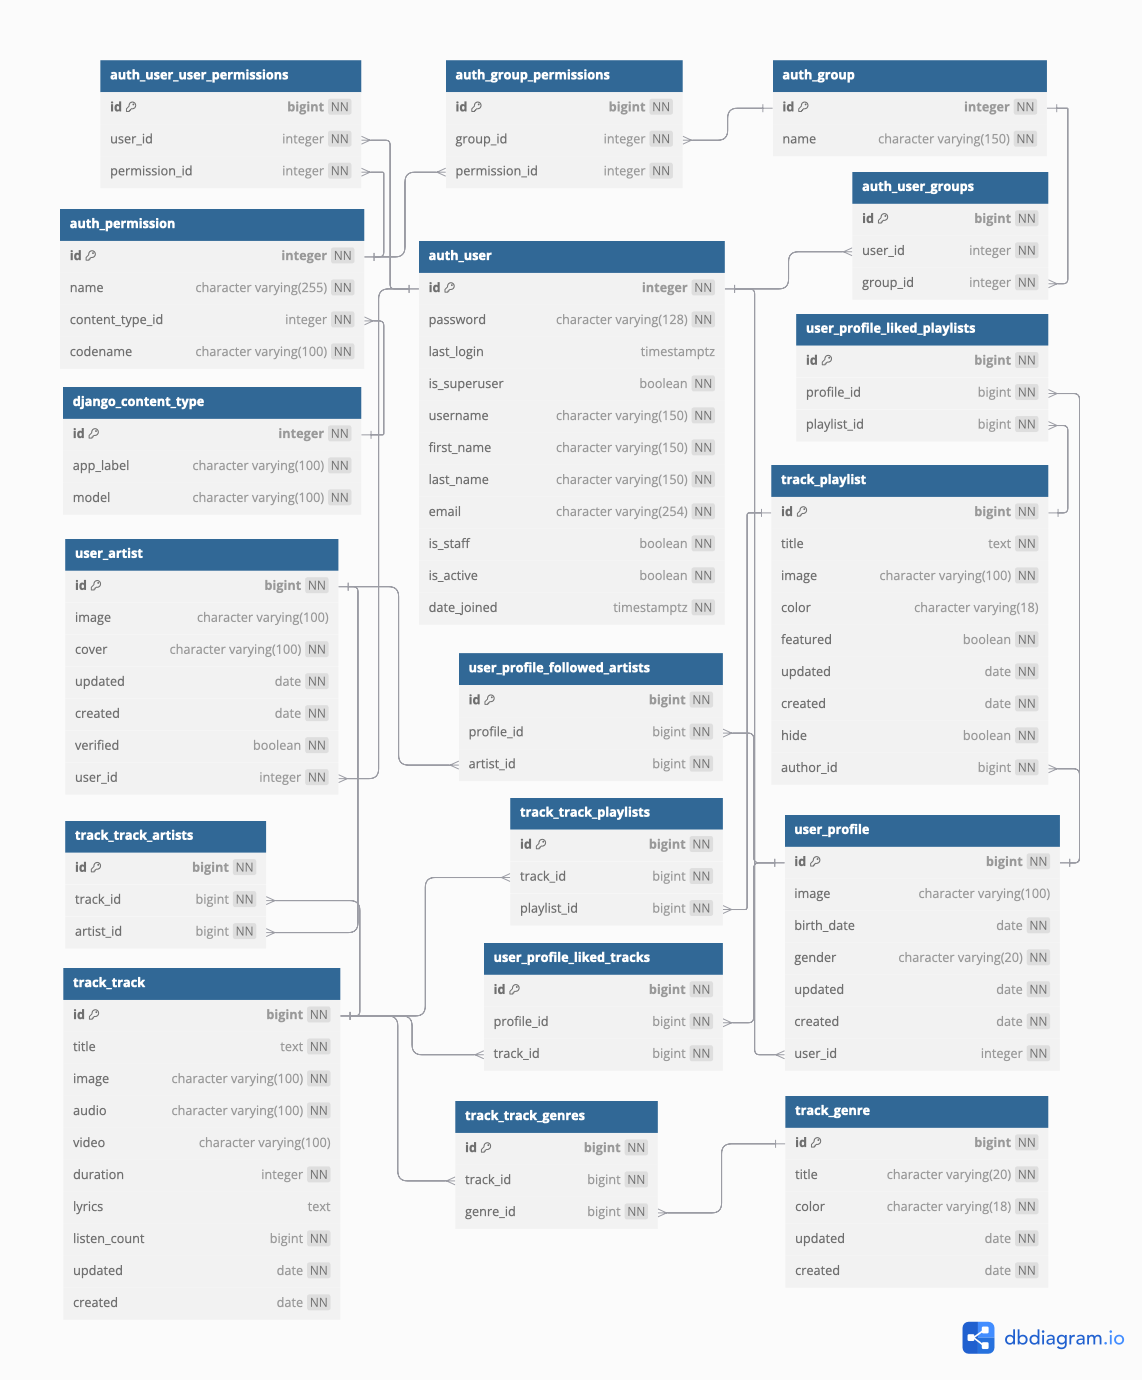
\includegraphics[width=12cm]{db.png}
\end{center}
\end{figure}
\newpage

\subsection{Cấu trúc dự án}
\subsubsection{Backend}
\begin{figure}[h!]
\begin{center}
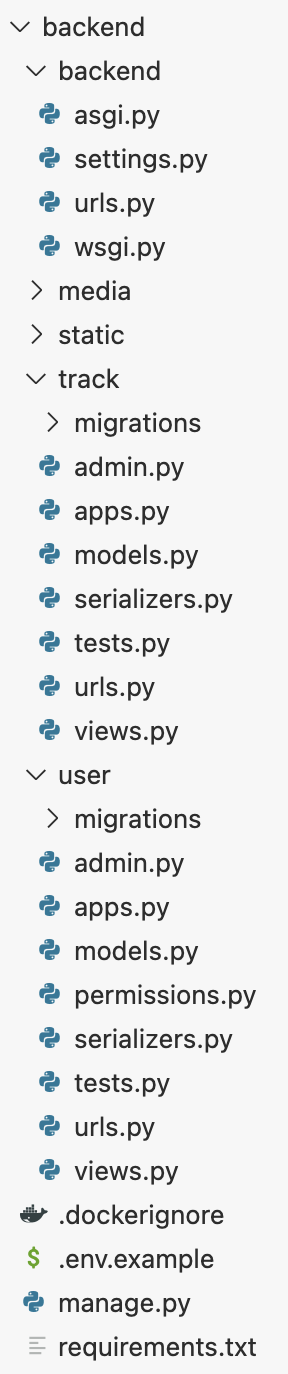
\includegraphics[width=4cm]{backend_folder.png}
\end{center}
\end{figure}
\newpage

\subsubsection{Frontend}
\begin{figure}[h!]
\begin{center}
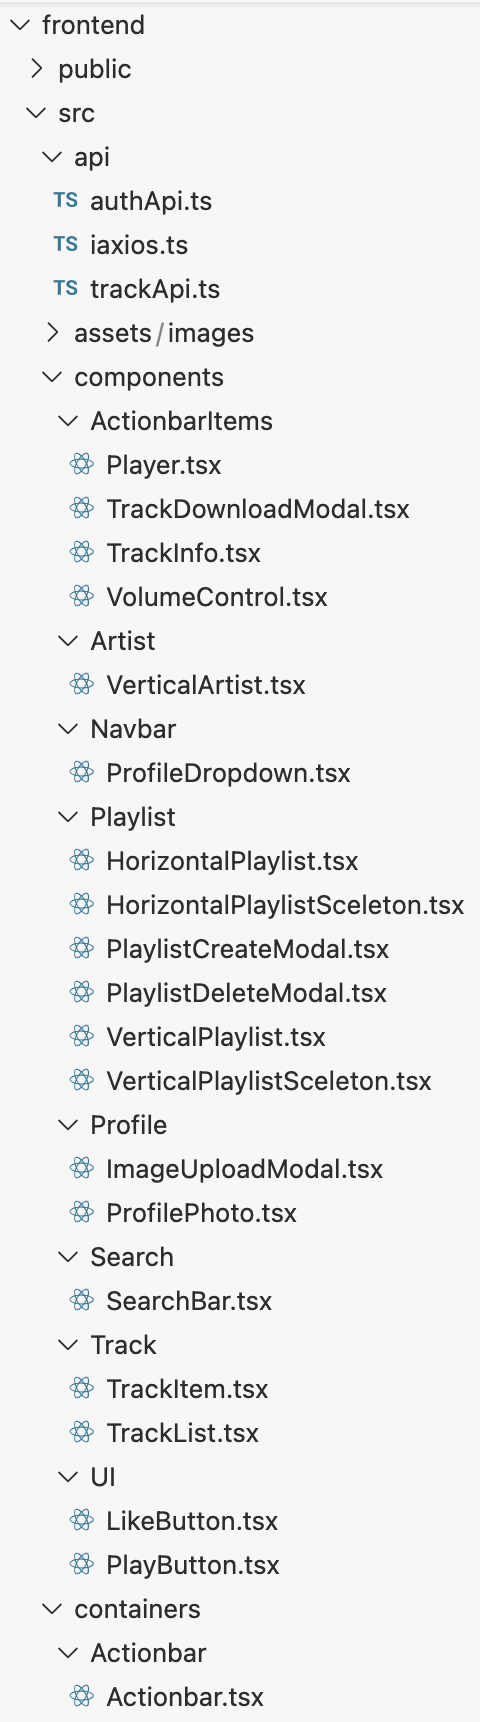
\includegraphics[width=5.5cm]{frontend_folder_1.png}
\end{center}
\end{figure}

\begin{figure}[h!]
\begin{center}
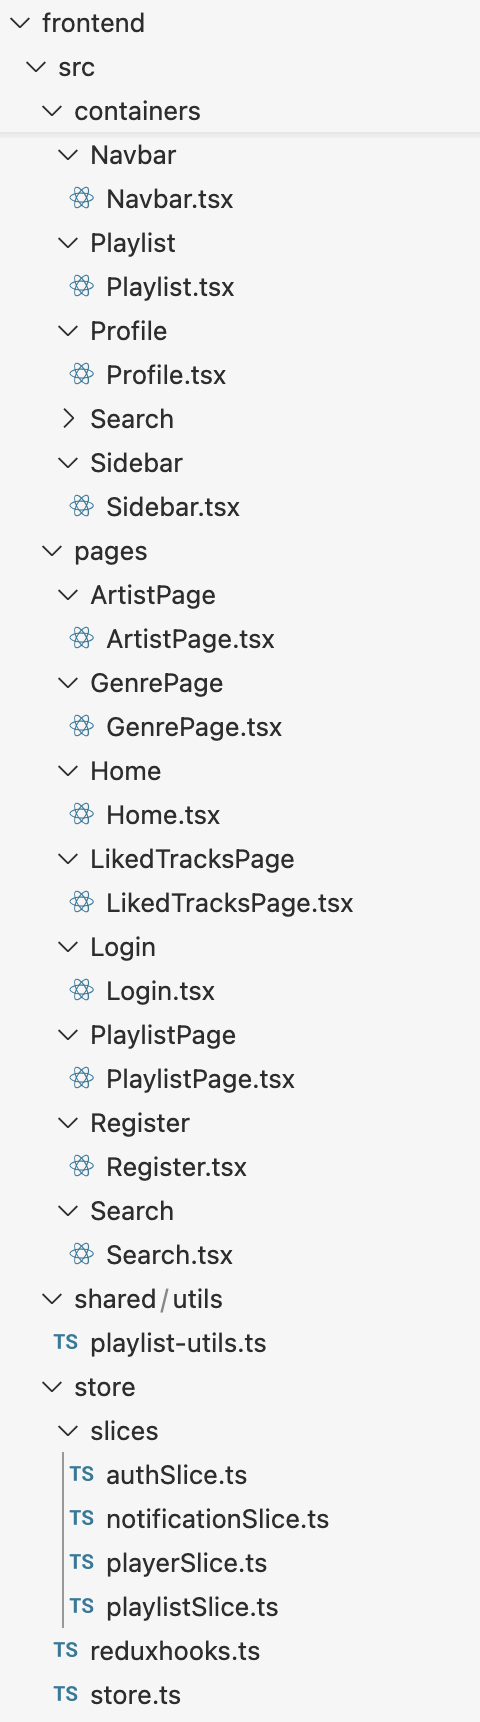
\includegraphics[width=5.5cm]{frontend_folder_2.png}
\end{center}
\end{figure}

\begin{figure}[h!]
\begin{center}
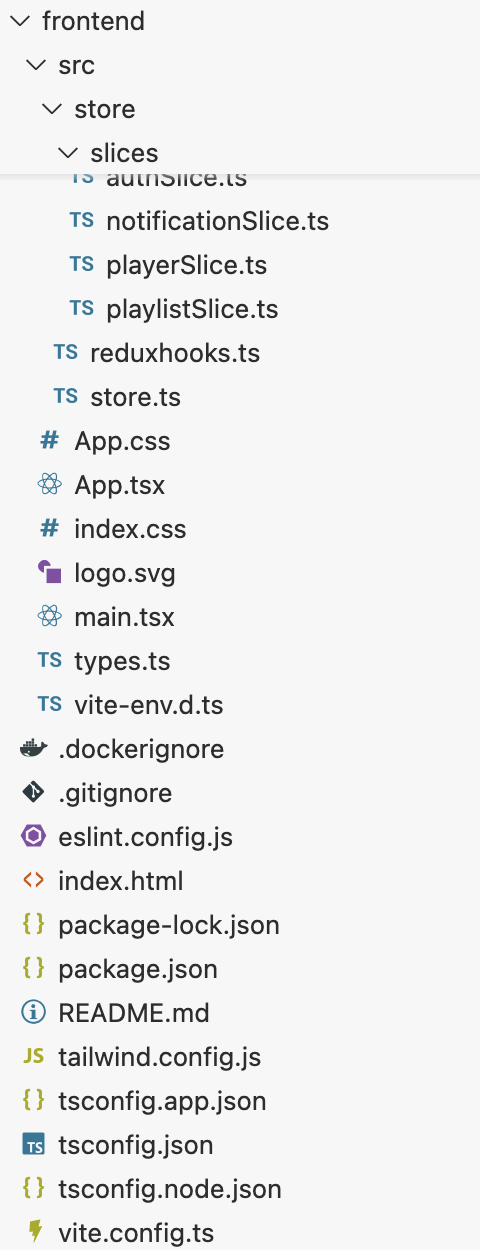
\includegraphics[width=5.5cm]{frontend_folder_3.png}
\end{center}
\end{figure}
\newpage

\subsection{Giao diện}
\newpage
\subsubsection{Trang chủ}

\begin{figure}[h!]
\begin{center}
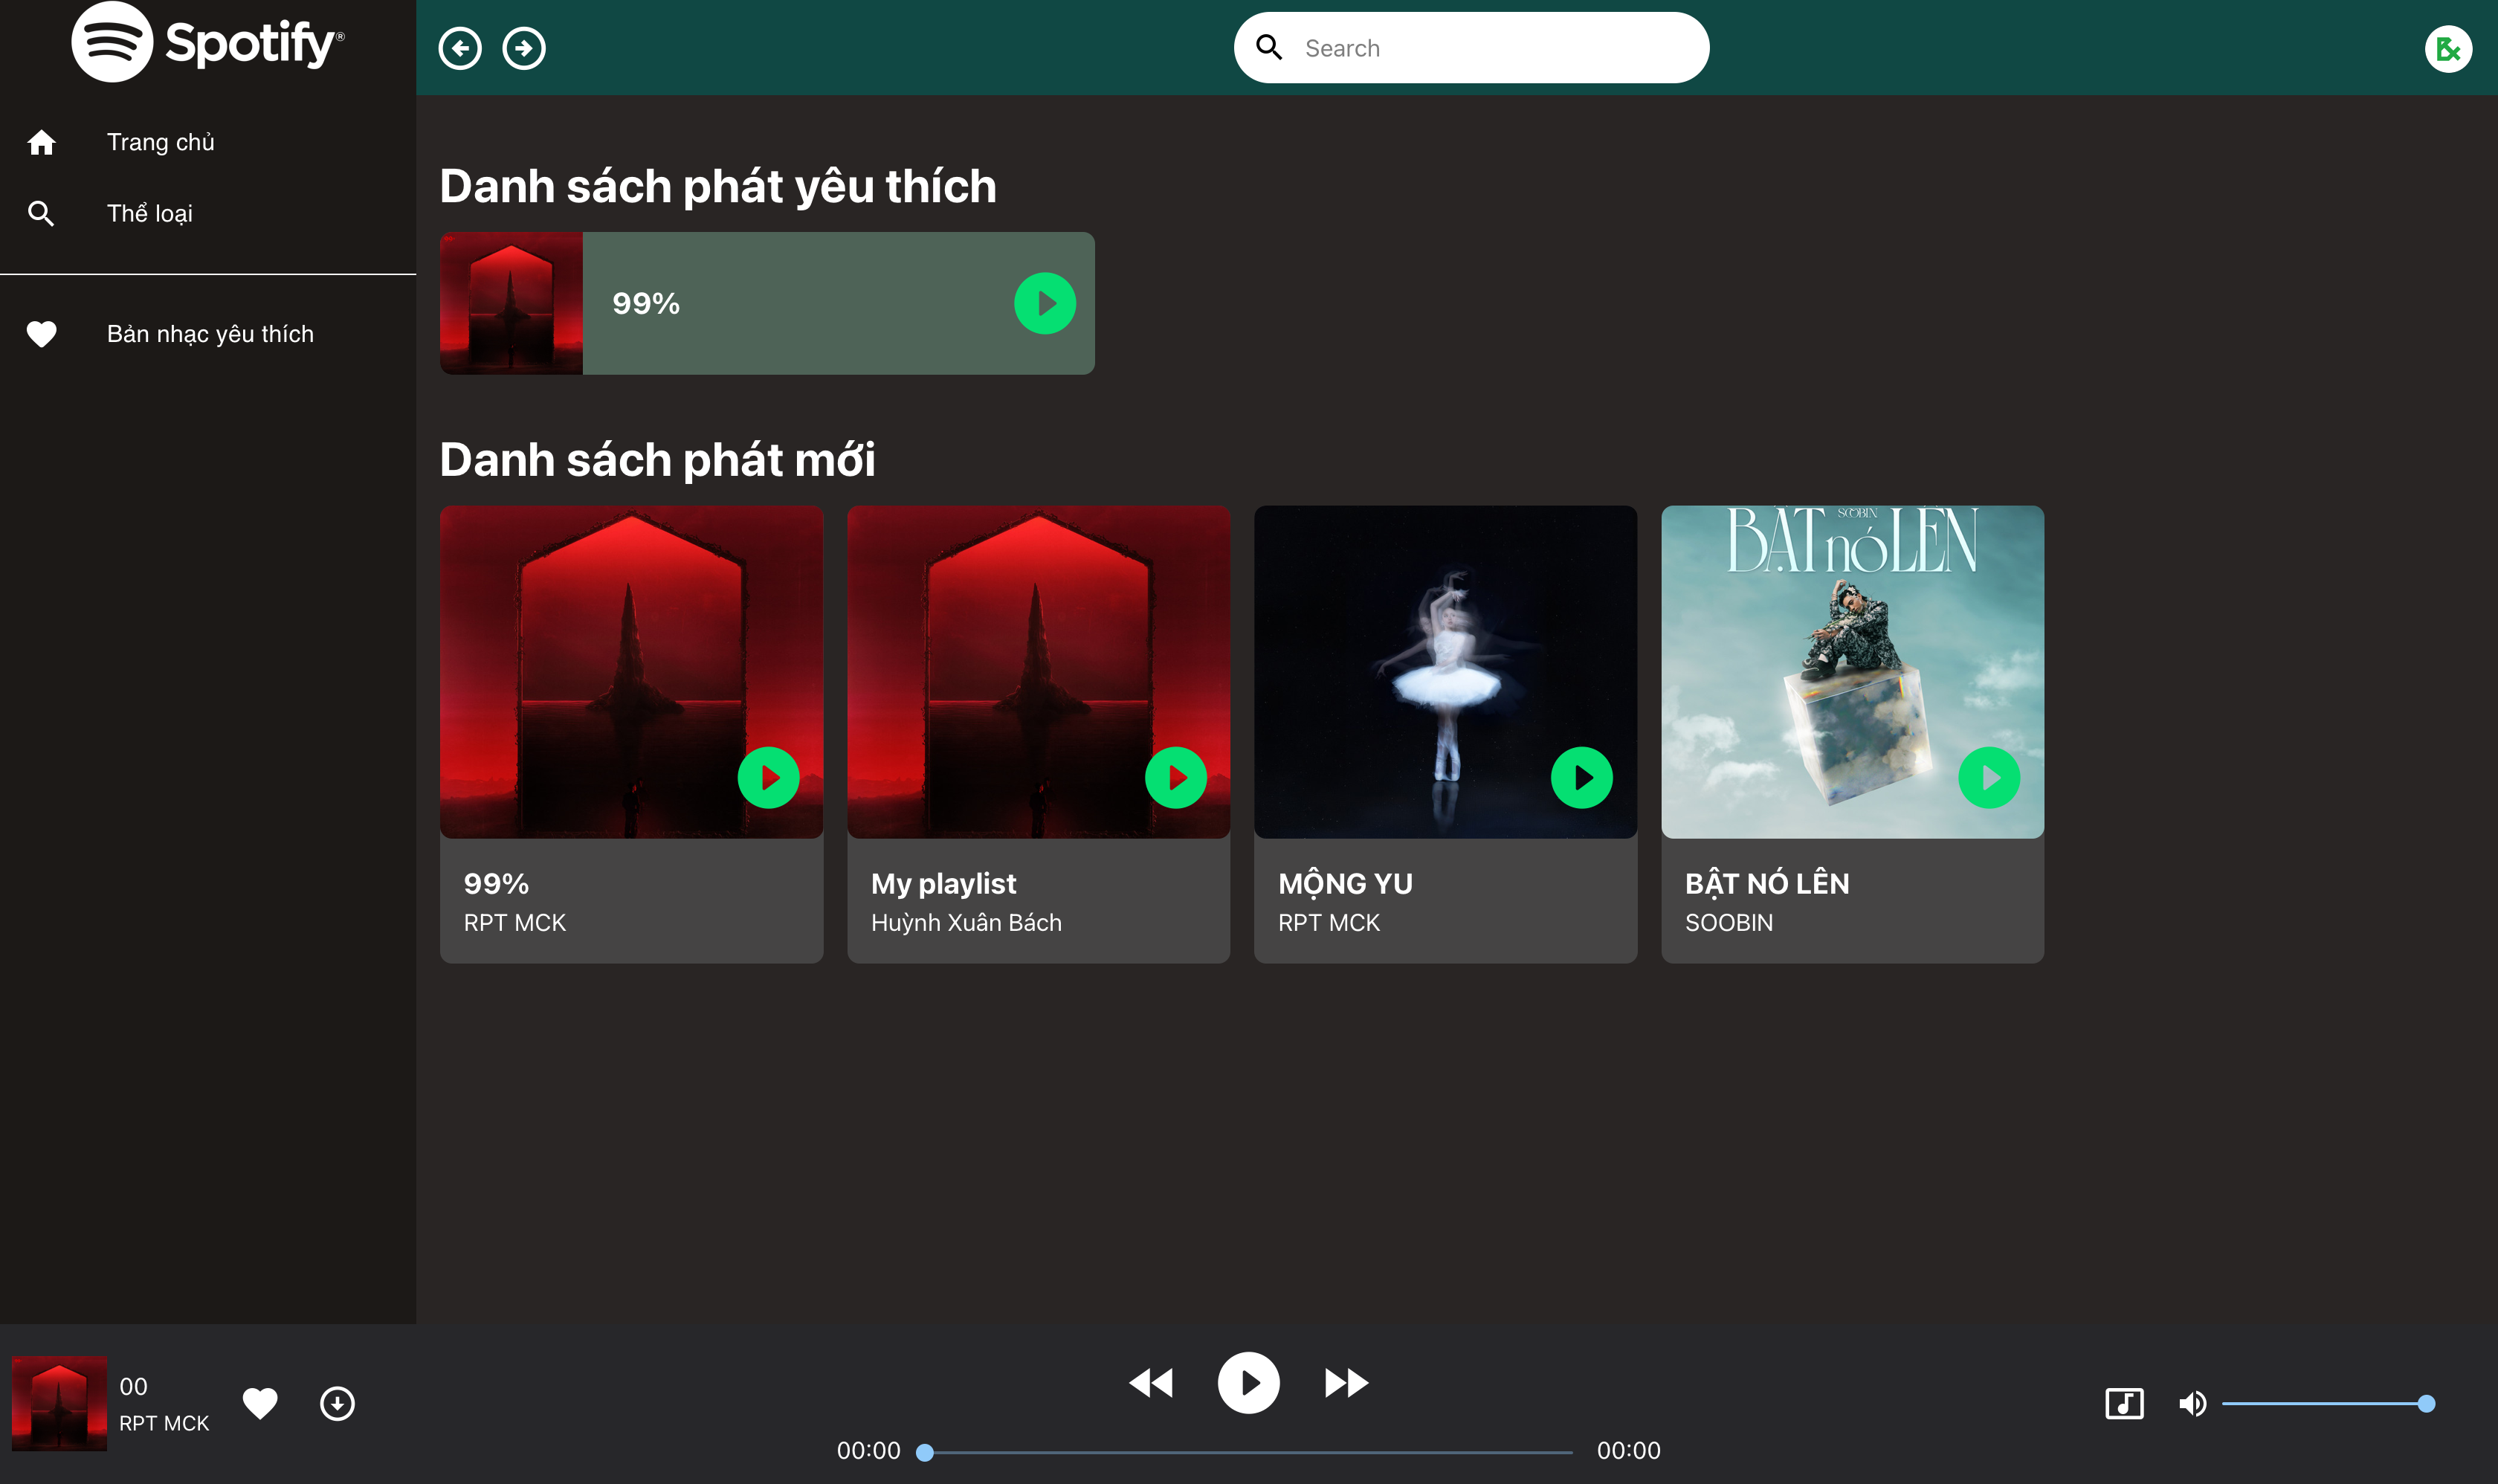
\includegraphics[width=12cm]{home.png}
\end{center}
\end{figure}

\subsubsection{Thể loại}
\begin{figure}[h!]
\begin{center}
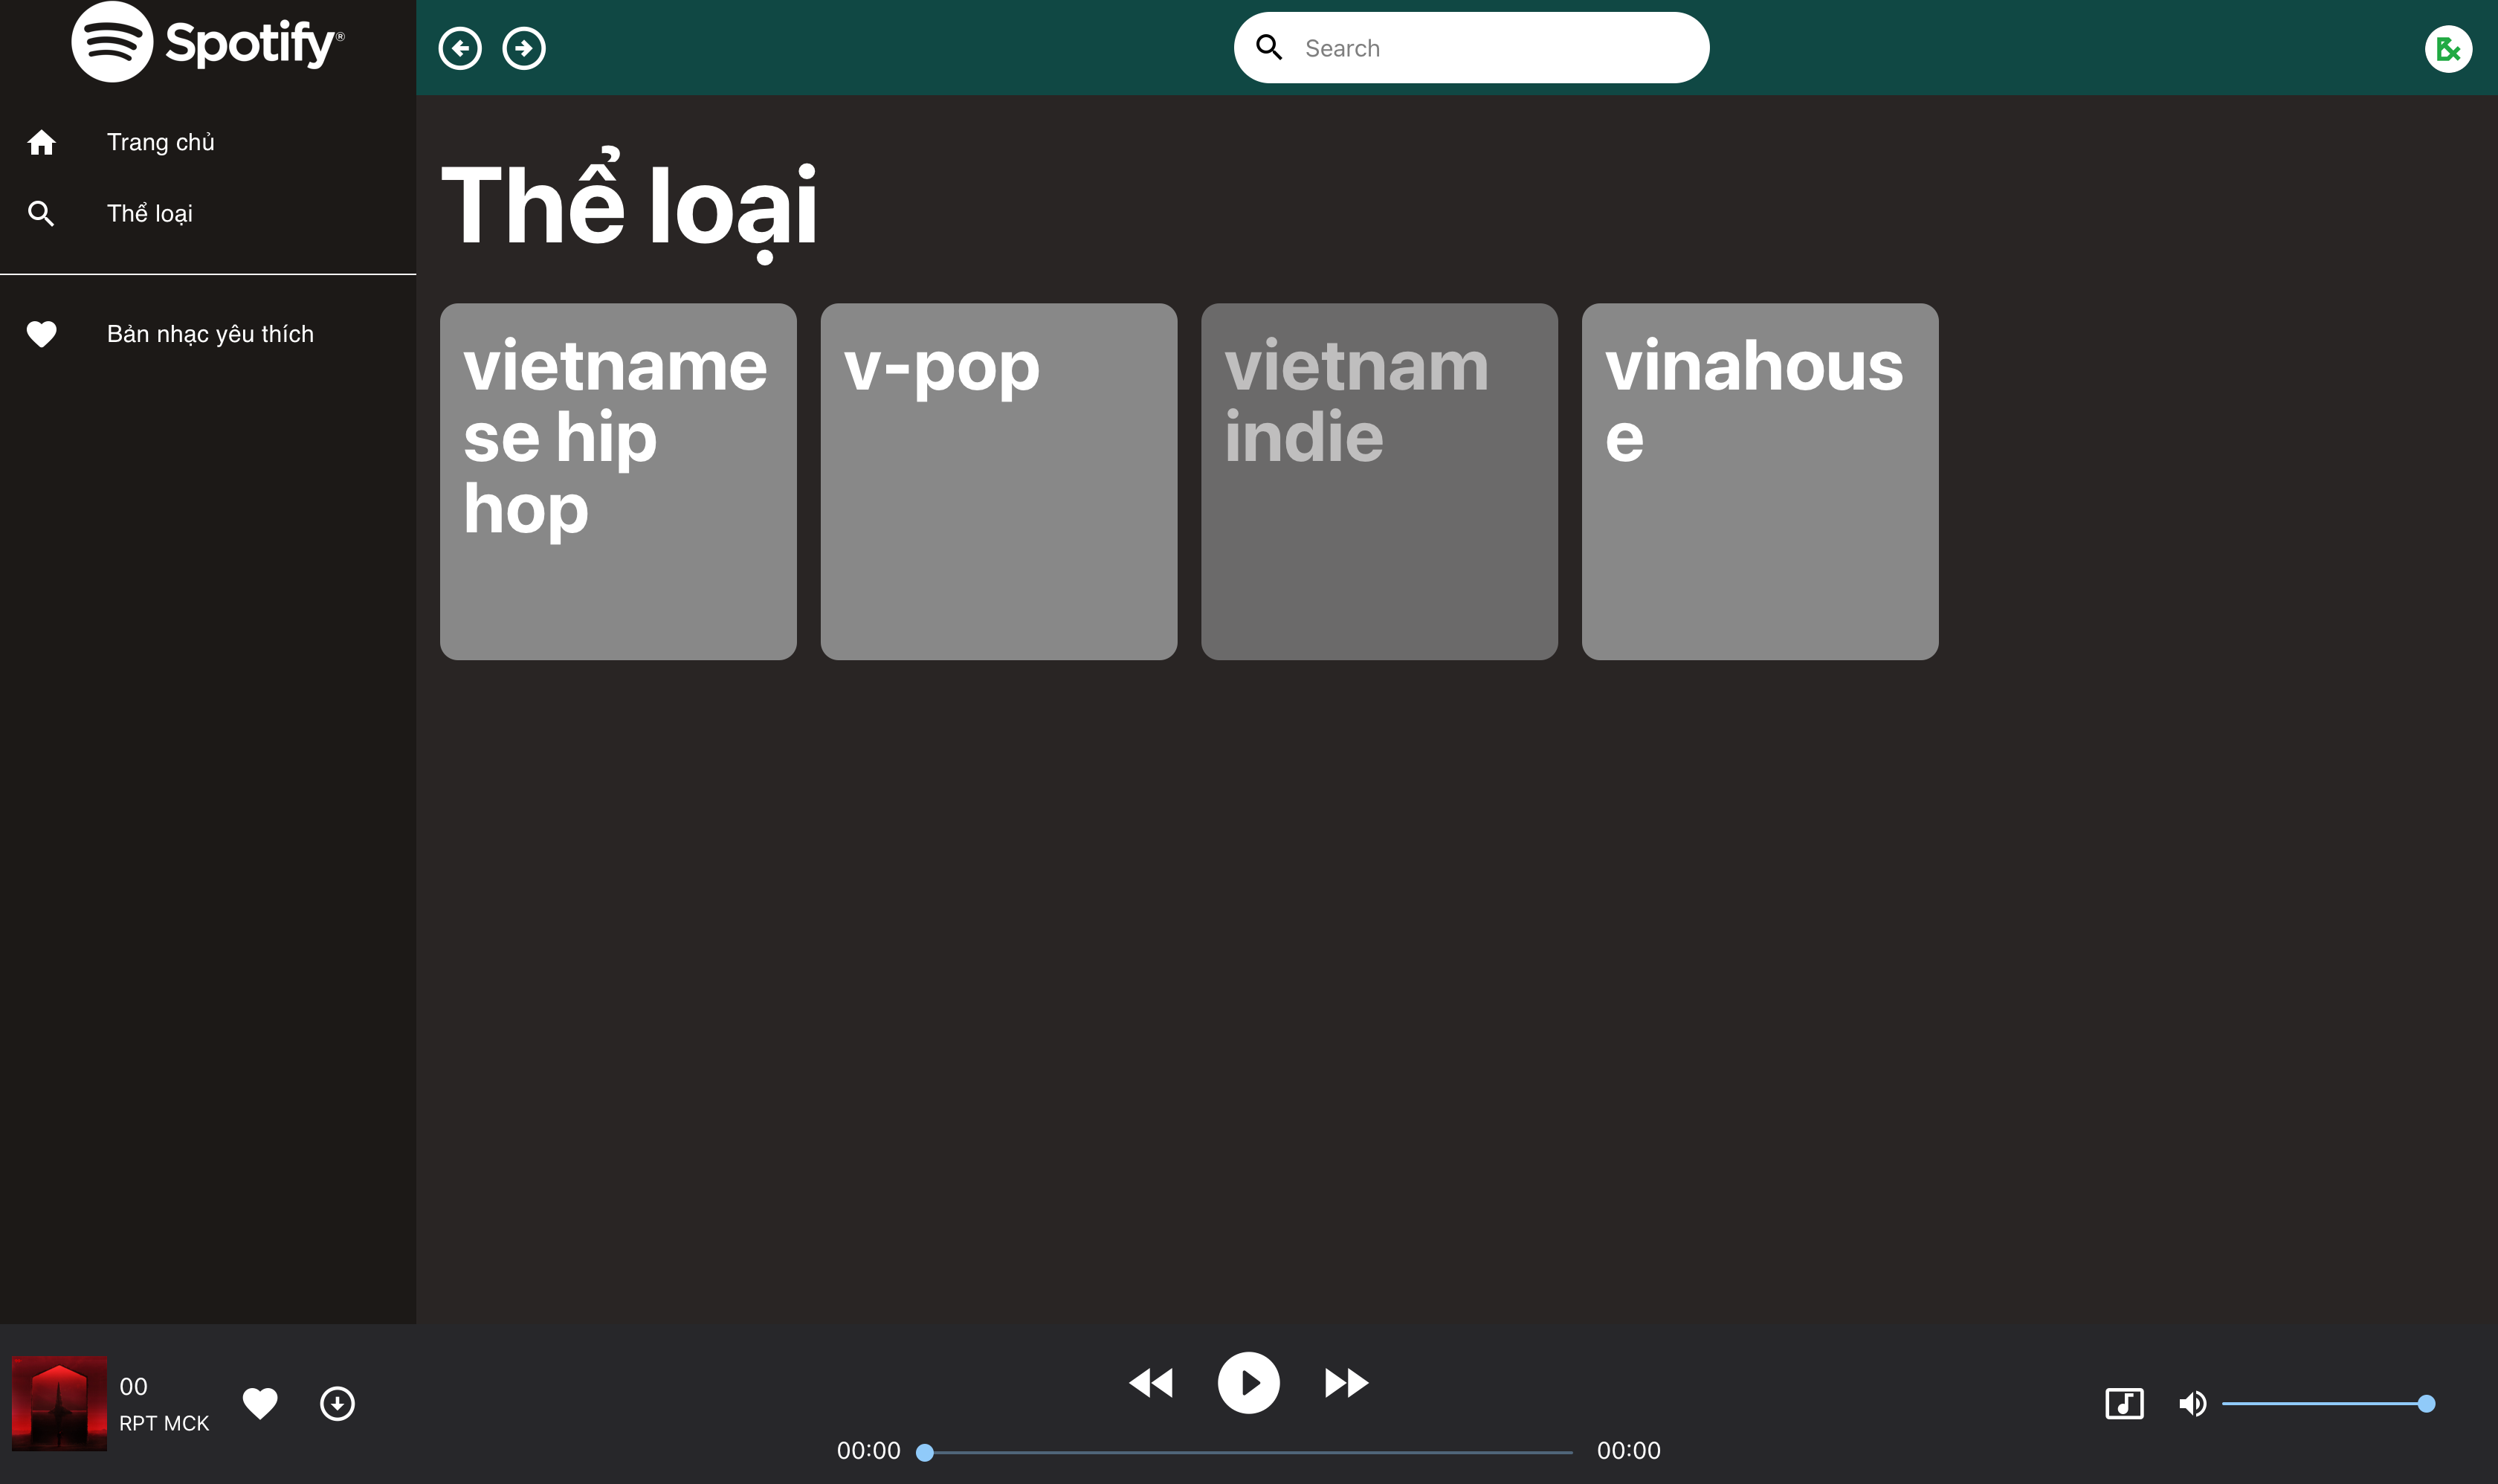
\includegraphics[width=12cm]{genres.png}
\end{center}
\end{figure}
\newpage

\subsubsection{Bản nhạc yêu thích}
\begin{figure}[h!]
\begin{center}
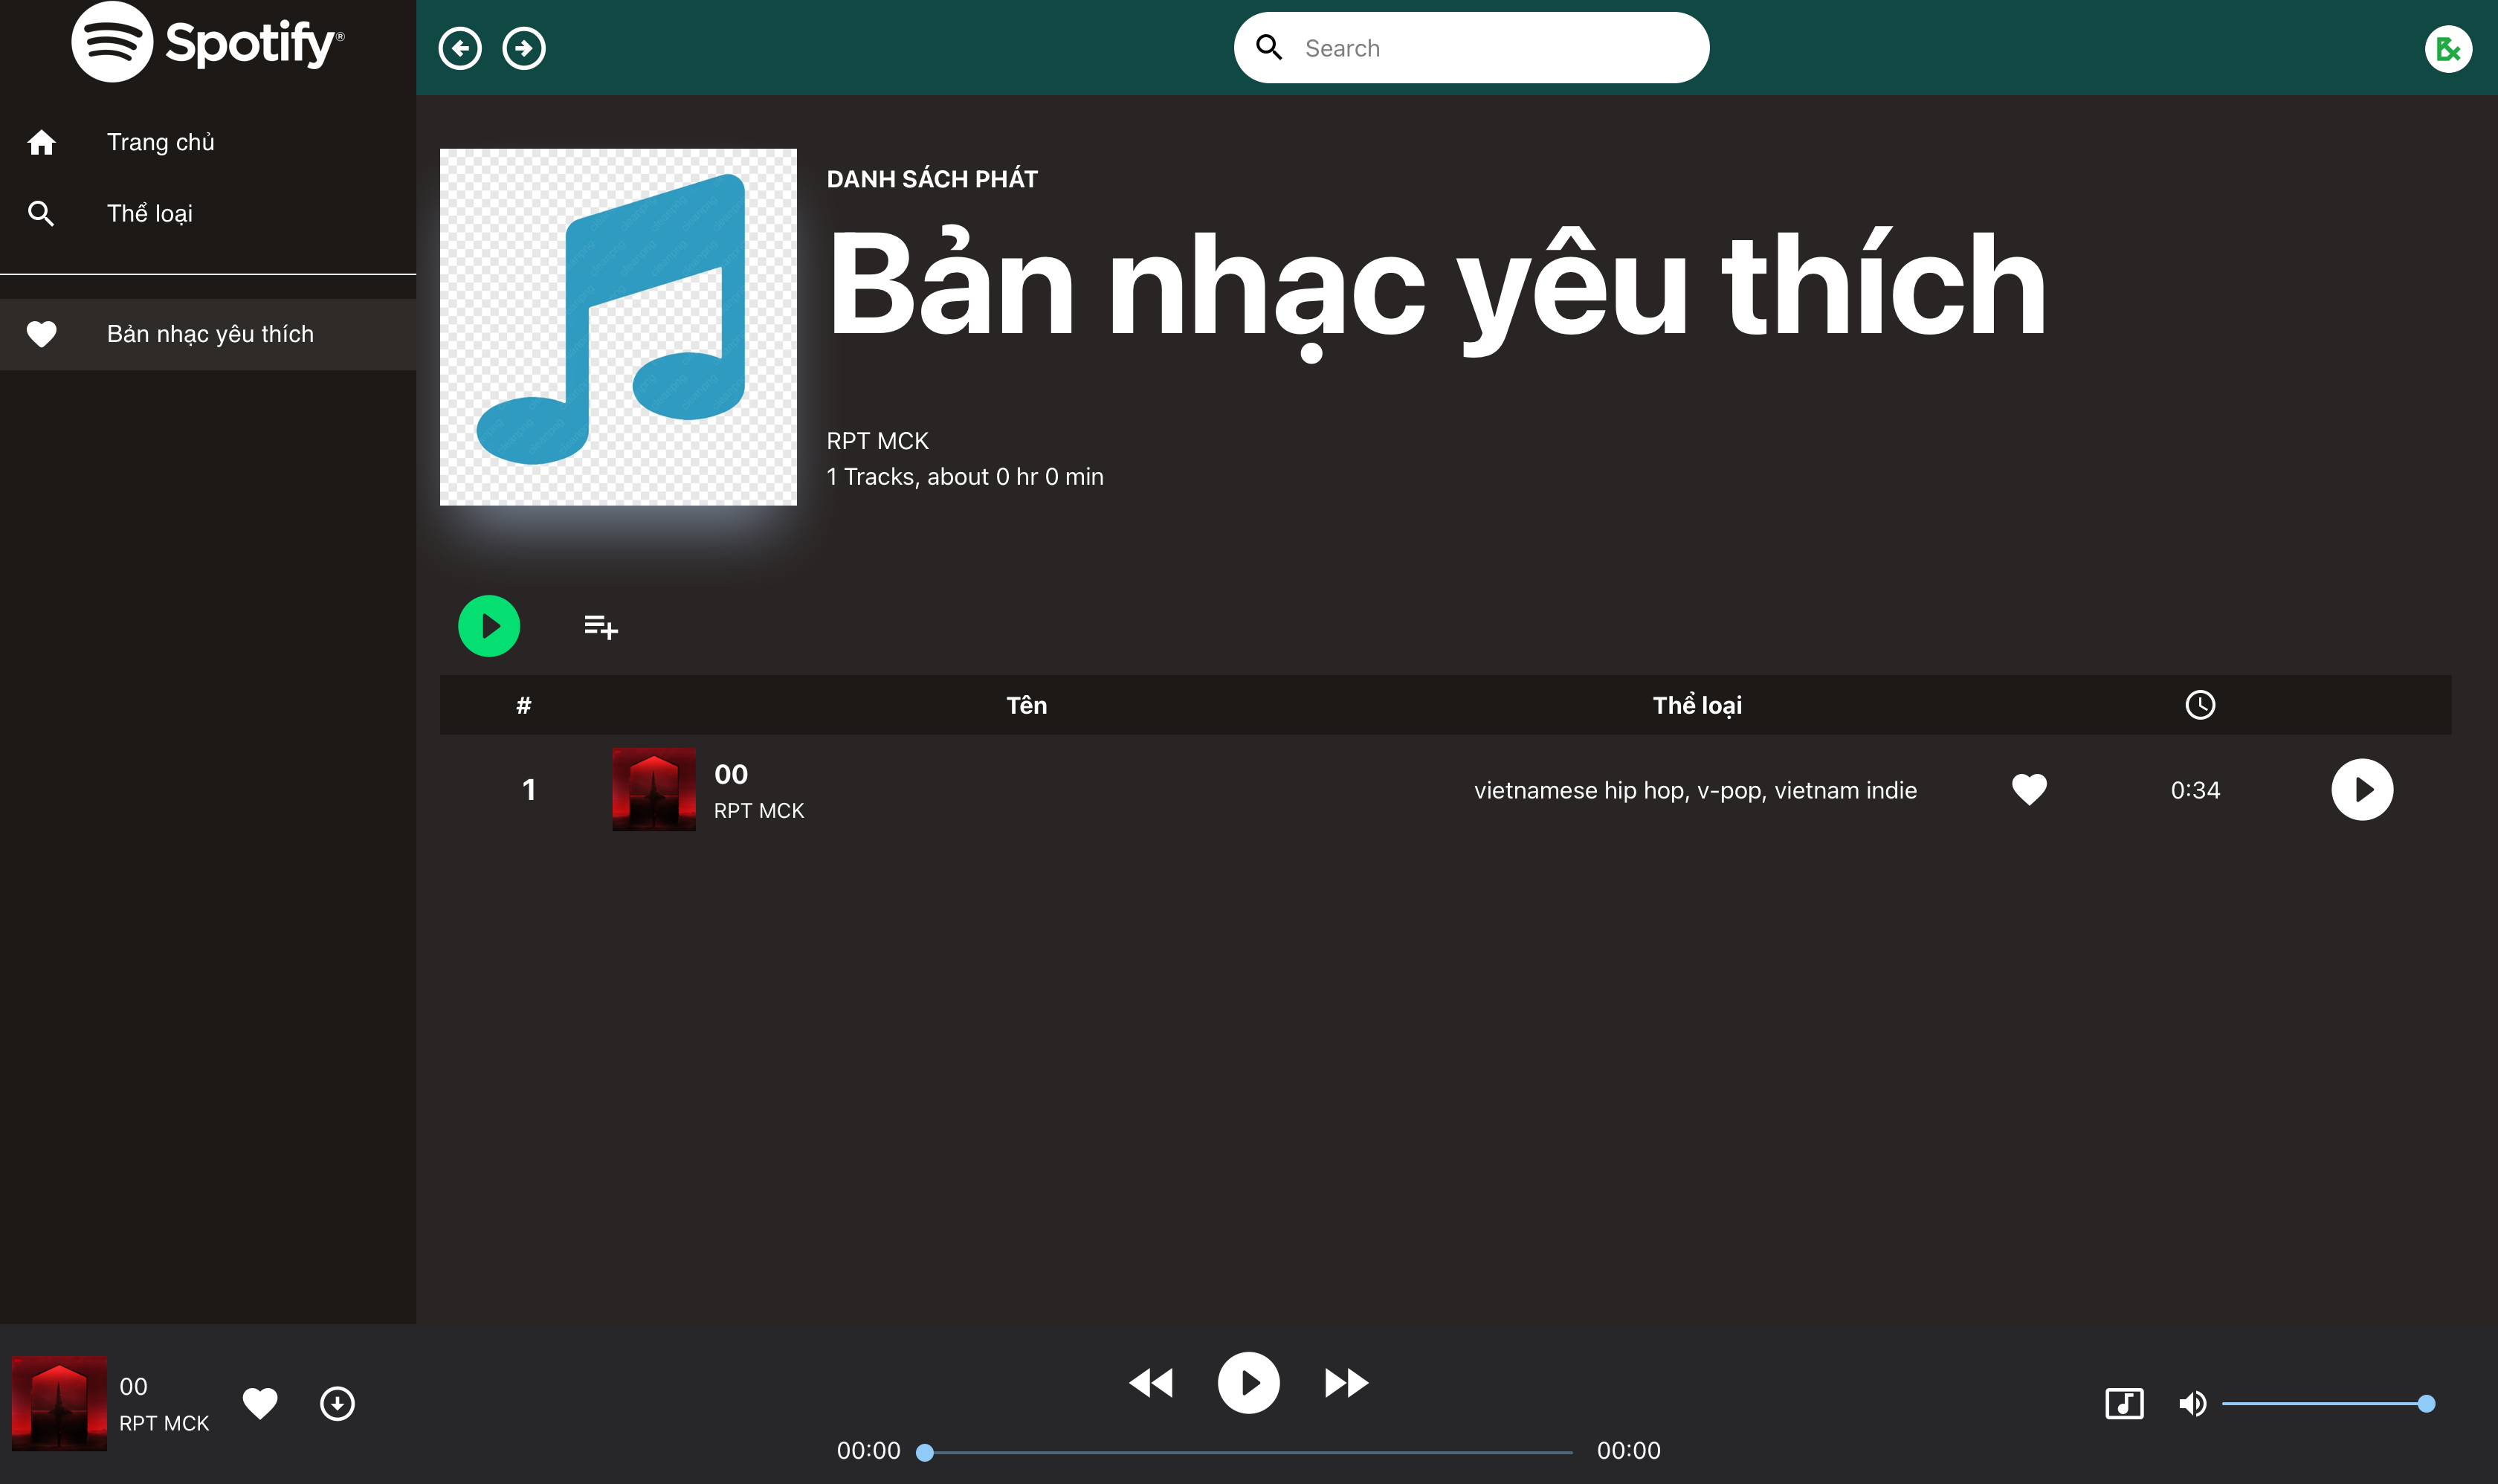
\includegraphics[width=12cm]{favorite.png}
\end{center}
\end{figure}

\subsubsection{Danh sách phát thể loại}
\begin{figure}[h!]
\begin{center}
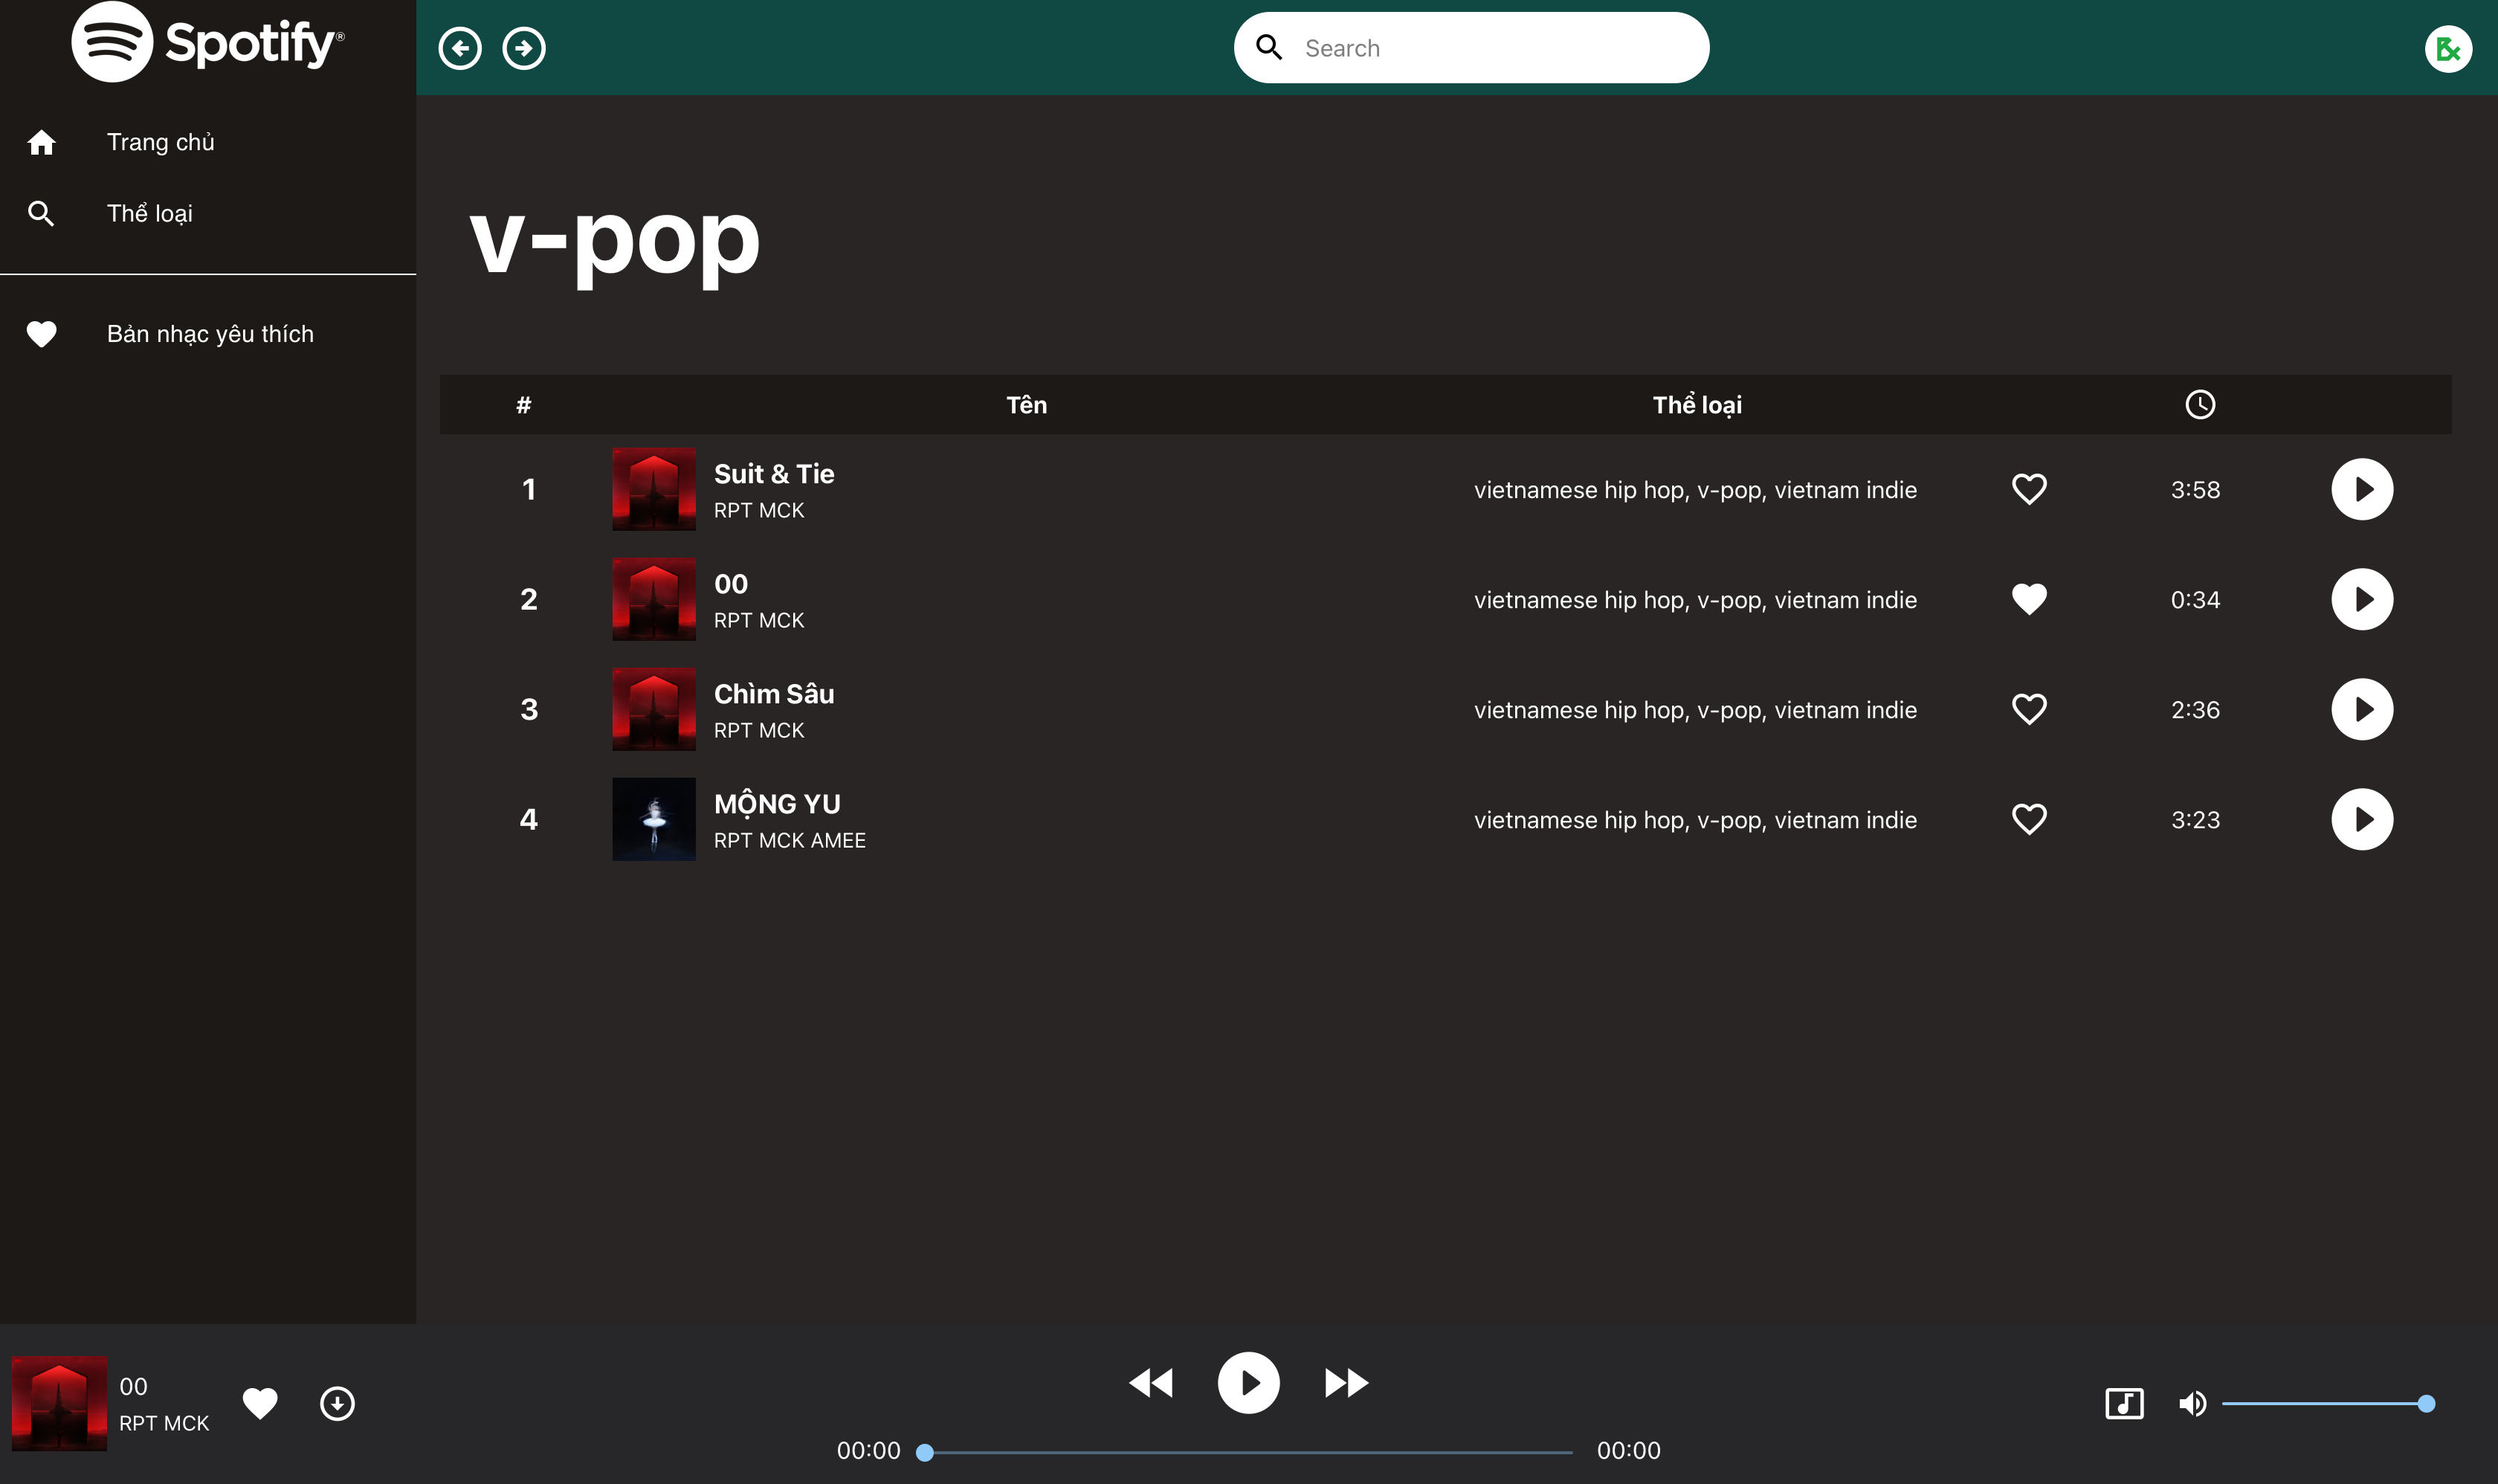
\includegraphics[width=12cm]{genres_playlist.png}
\end{center}
\end{figure}
\newpage

\subsubsection{Danh sách phát}
\begin{figure}[h!]
\begin{center}
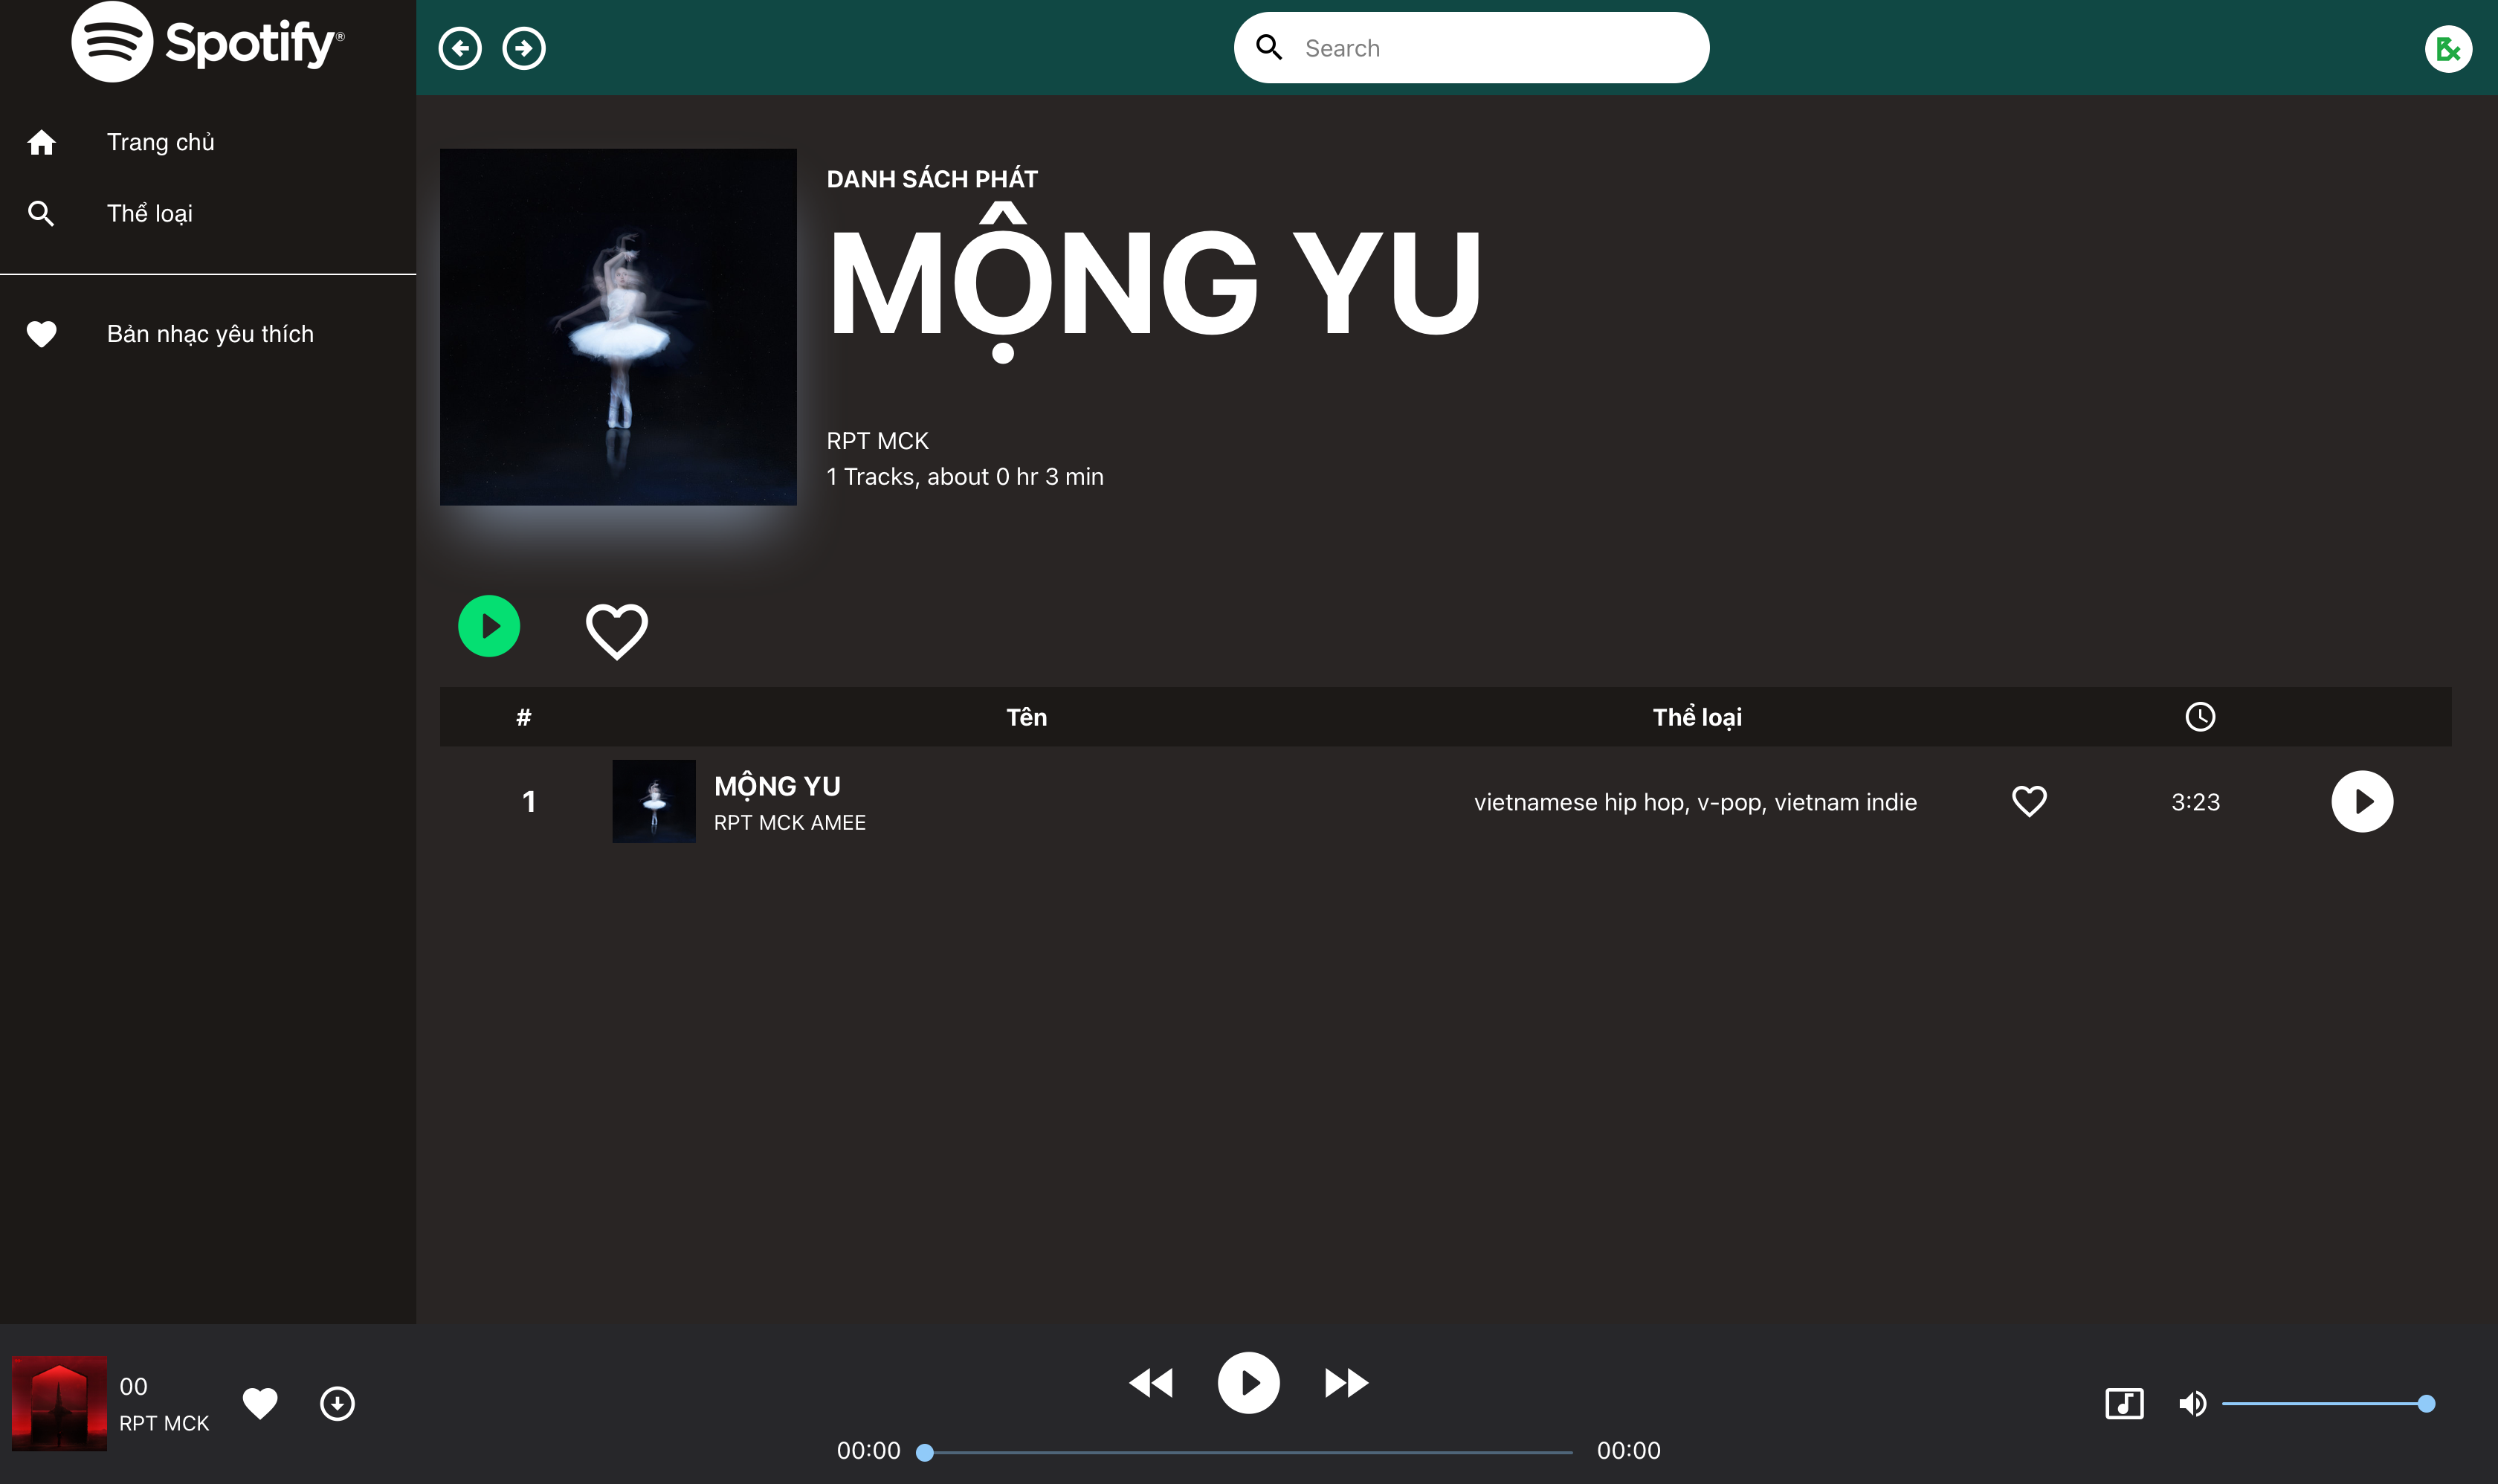
\includegraphics[width=12cm]{playlist.png}
\end{center}
\end{figure}

\subsubsection{Tìm kiếm}
\begin{figure}[h!]
\begin{center}
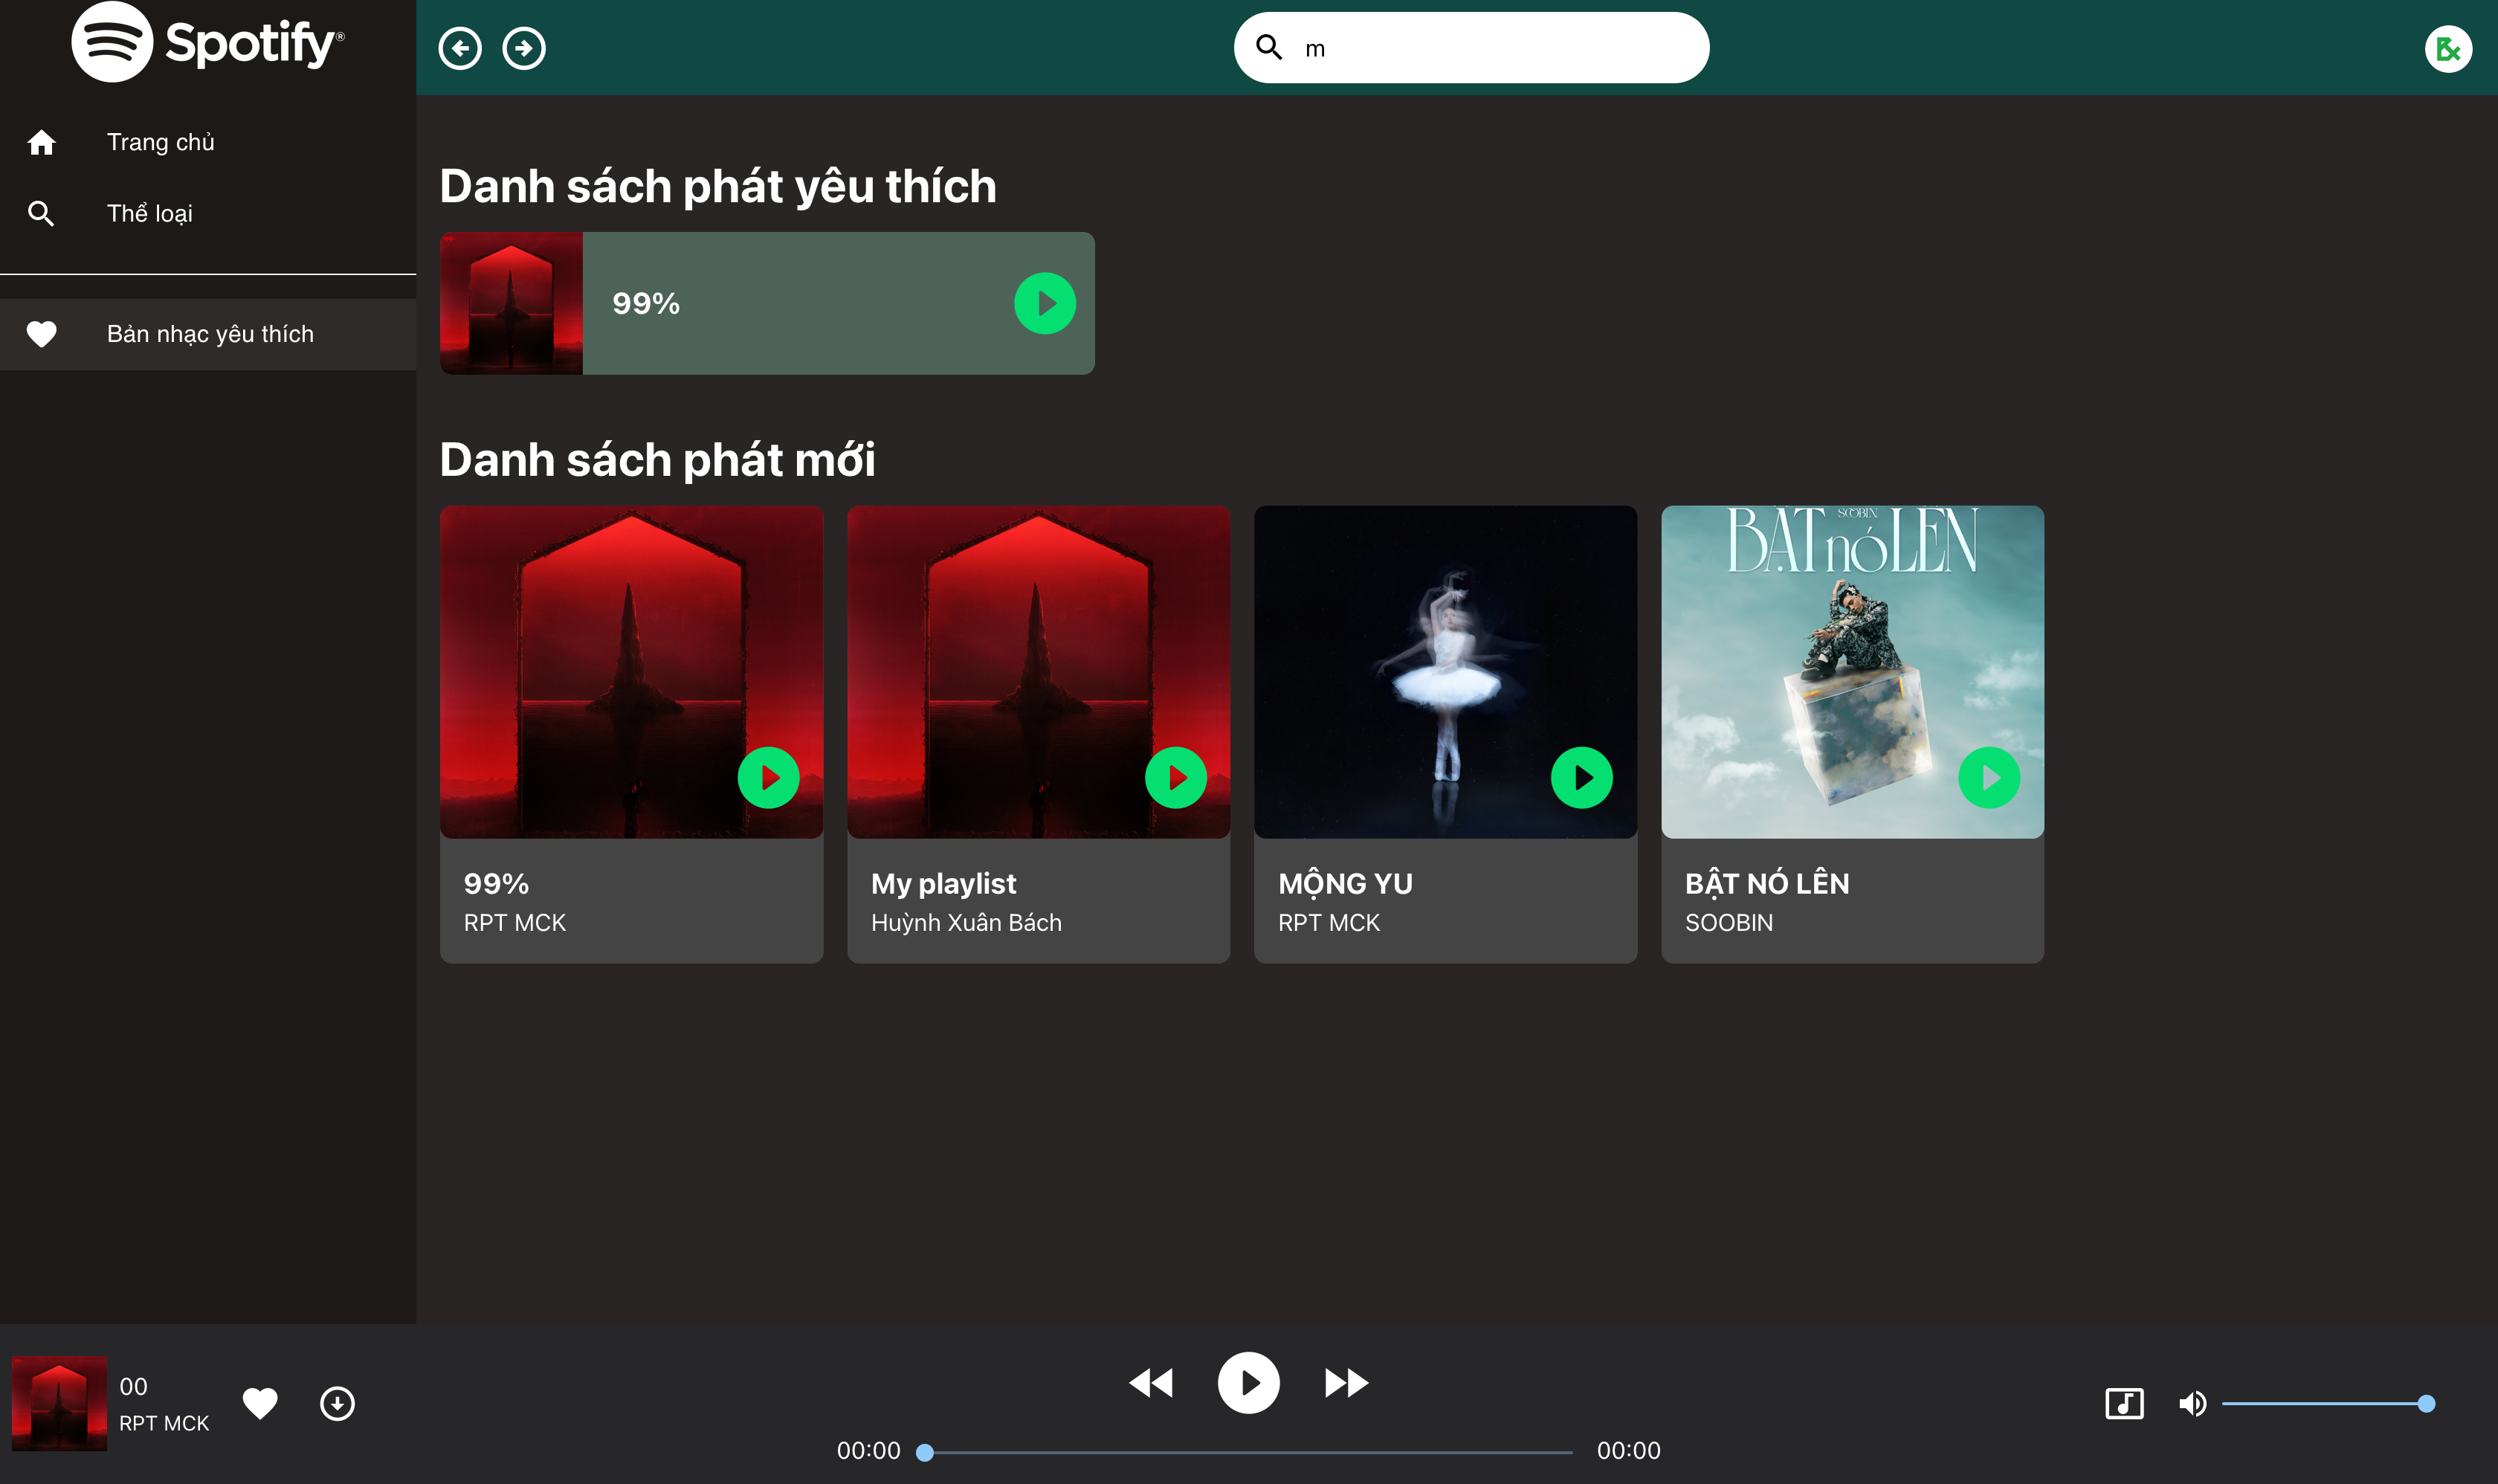
\includegraphics[width=12cm]{searching.png}
\end{center}
\end{figure}
\newpage

\subsubsection{Nghệ sĩ}
\begin{figure}[h!]
\begin{center}
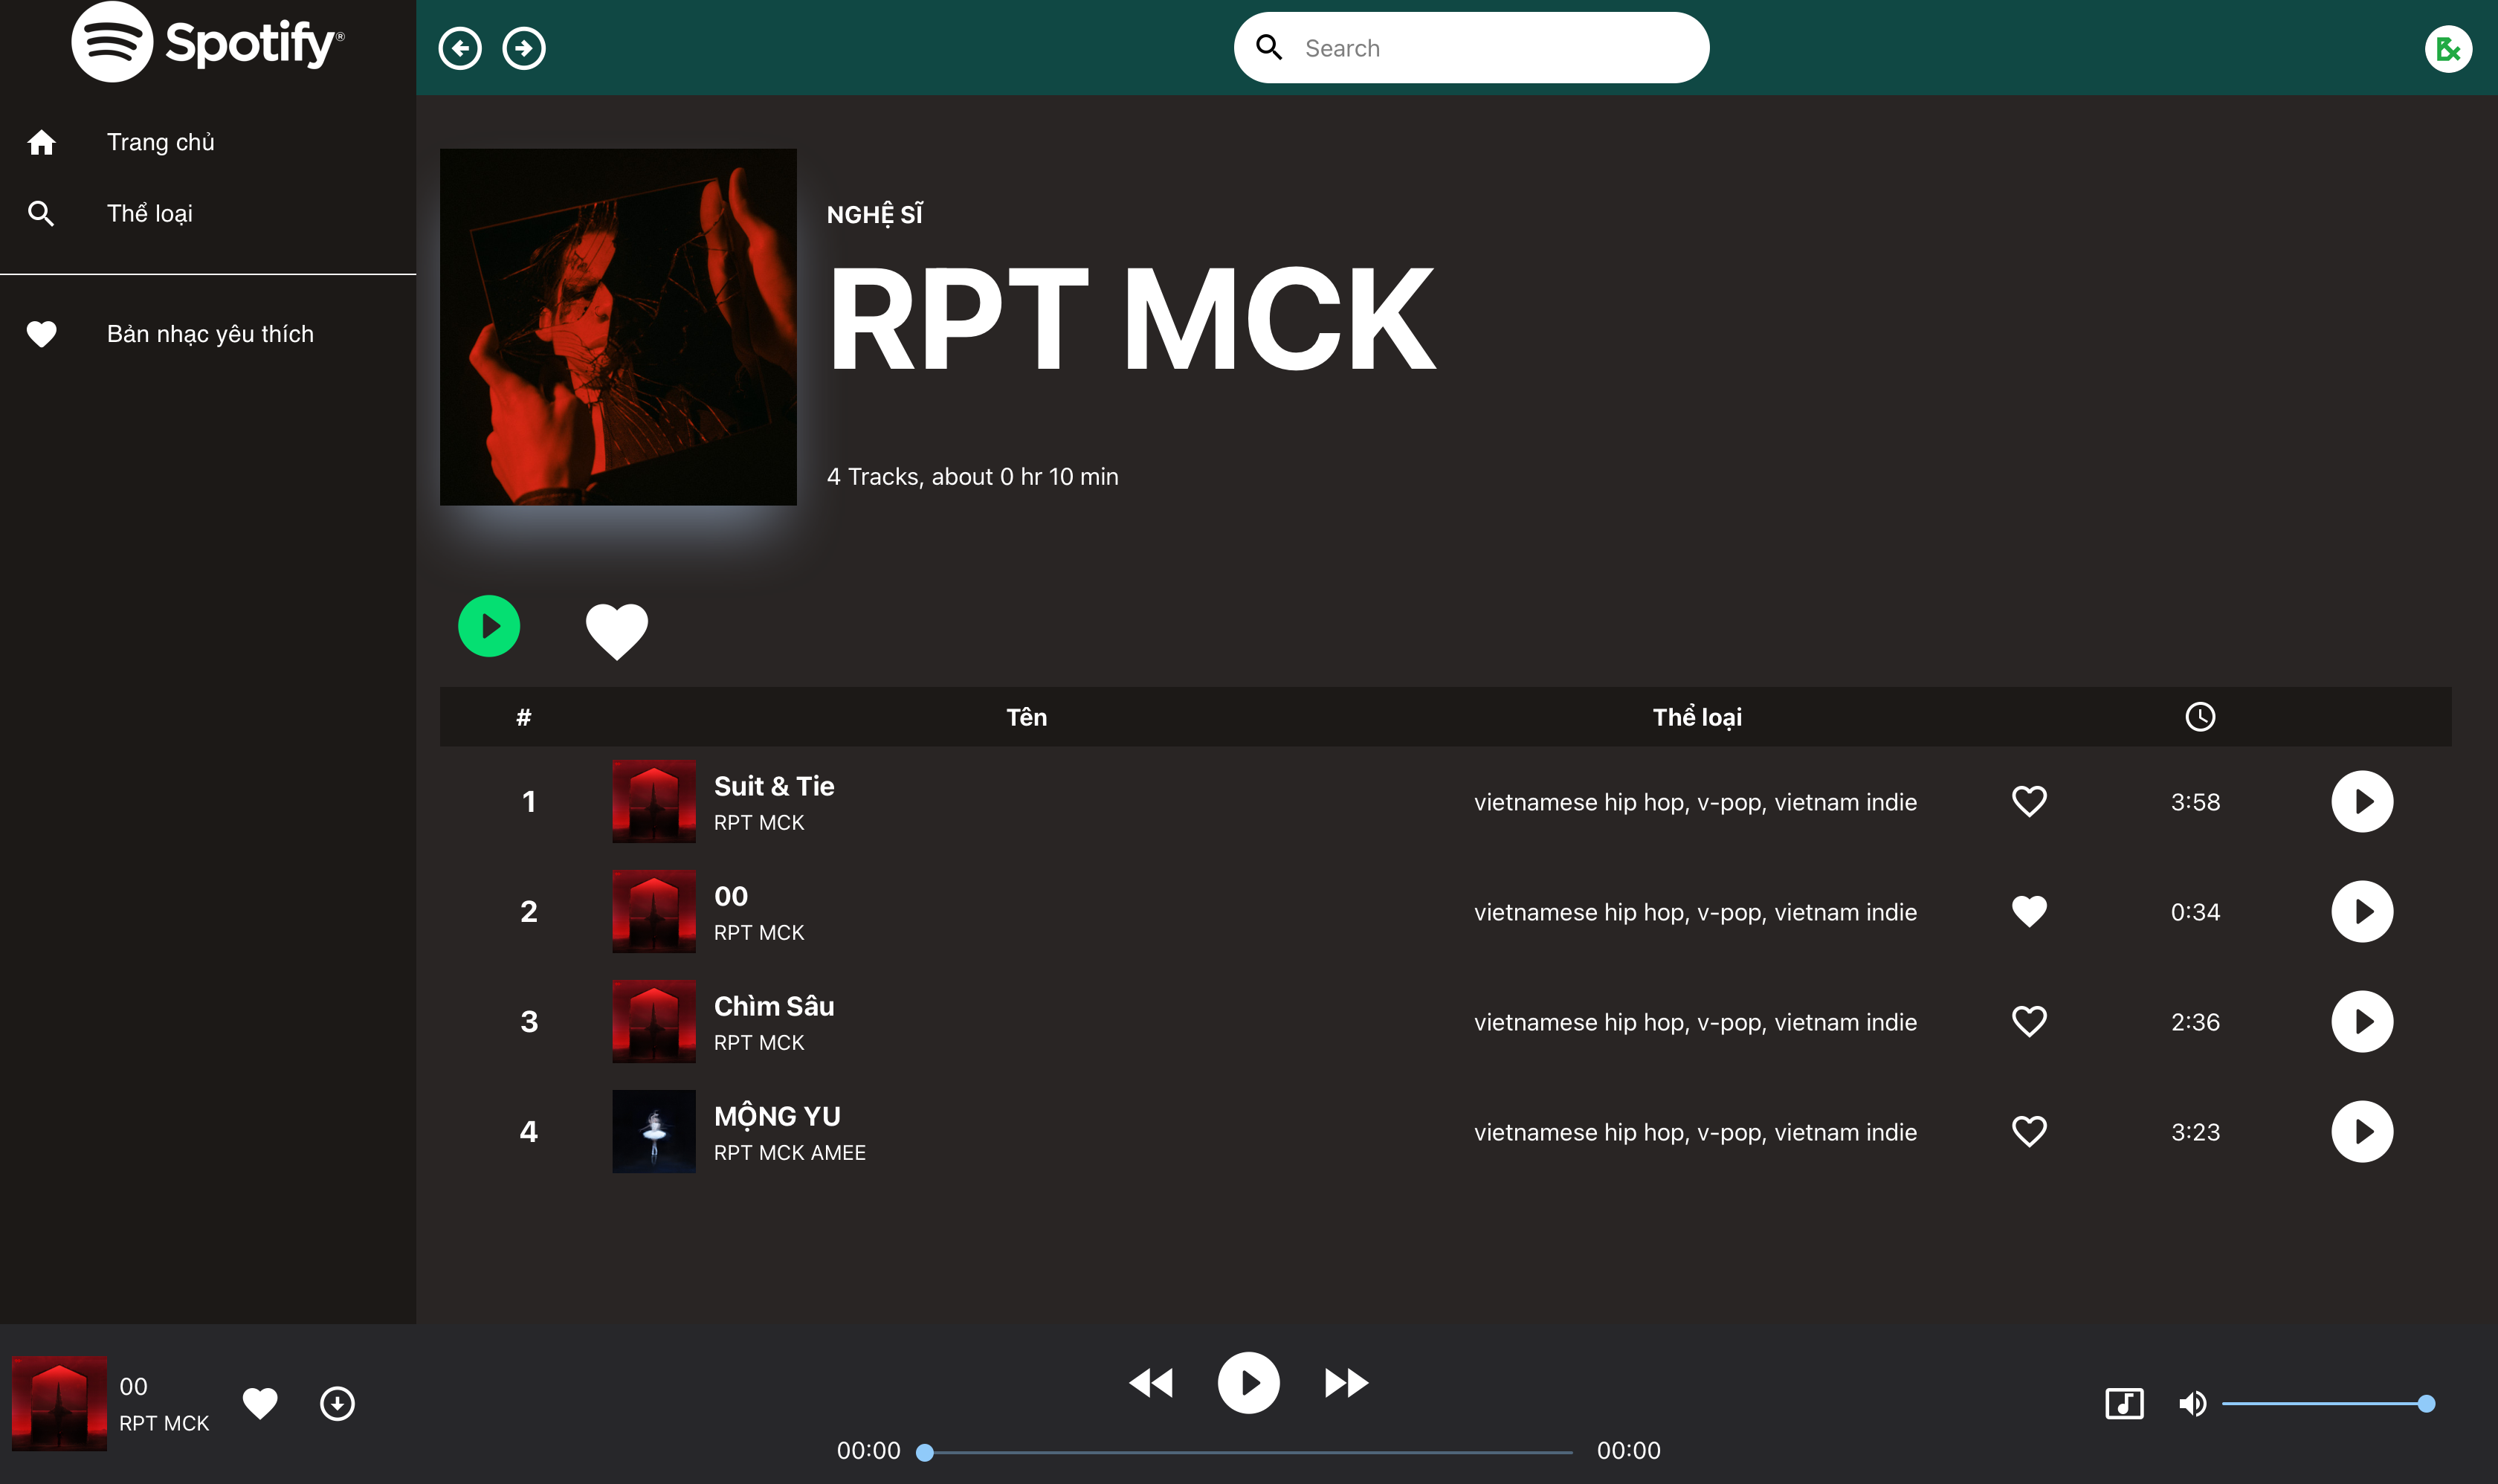
\includegraphics[width=12cm]{artist.png}
\end{center}
\end{figure}

\subsubsection{Hồ sơ}
\begin{figure}[h!]
\begin{center}
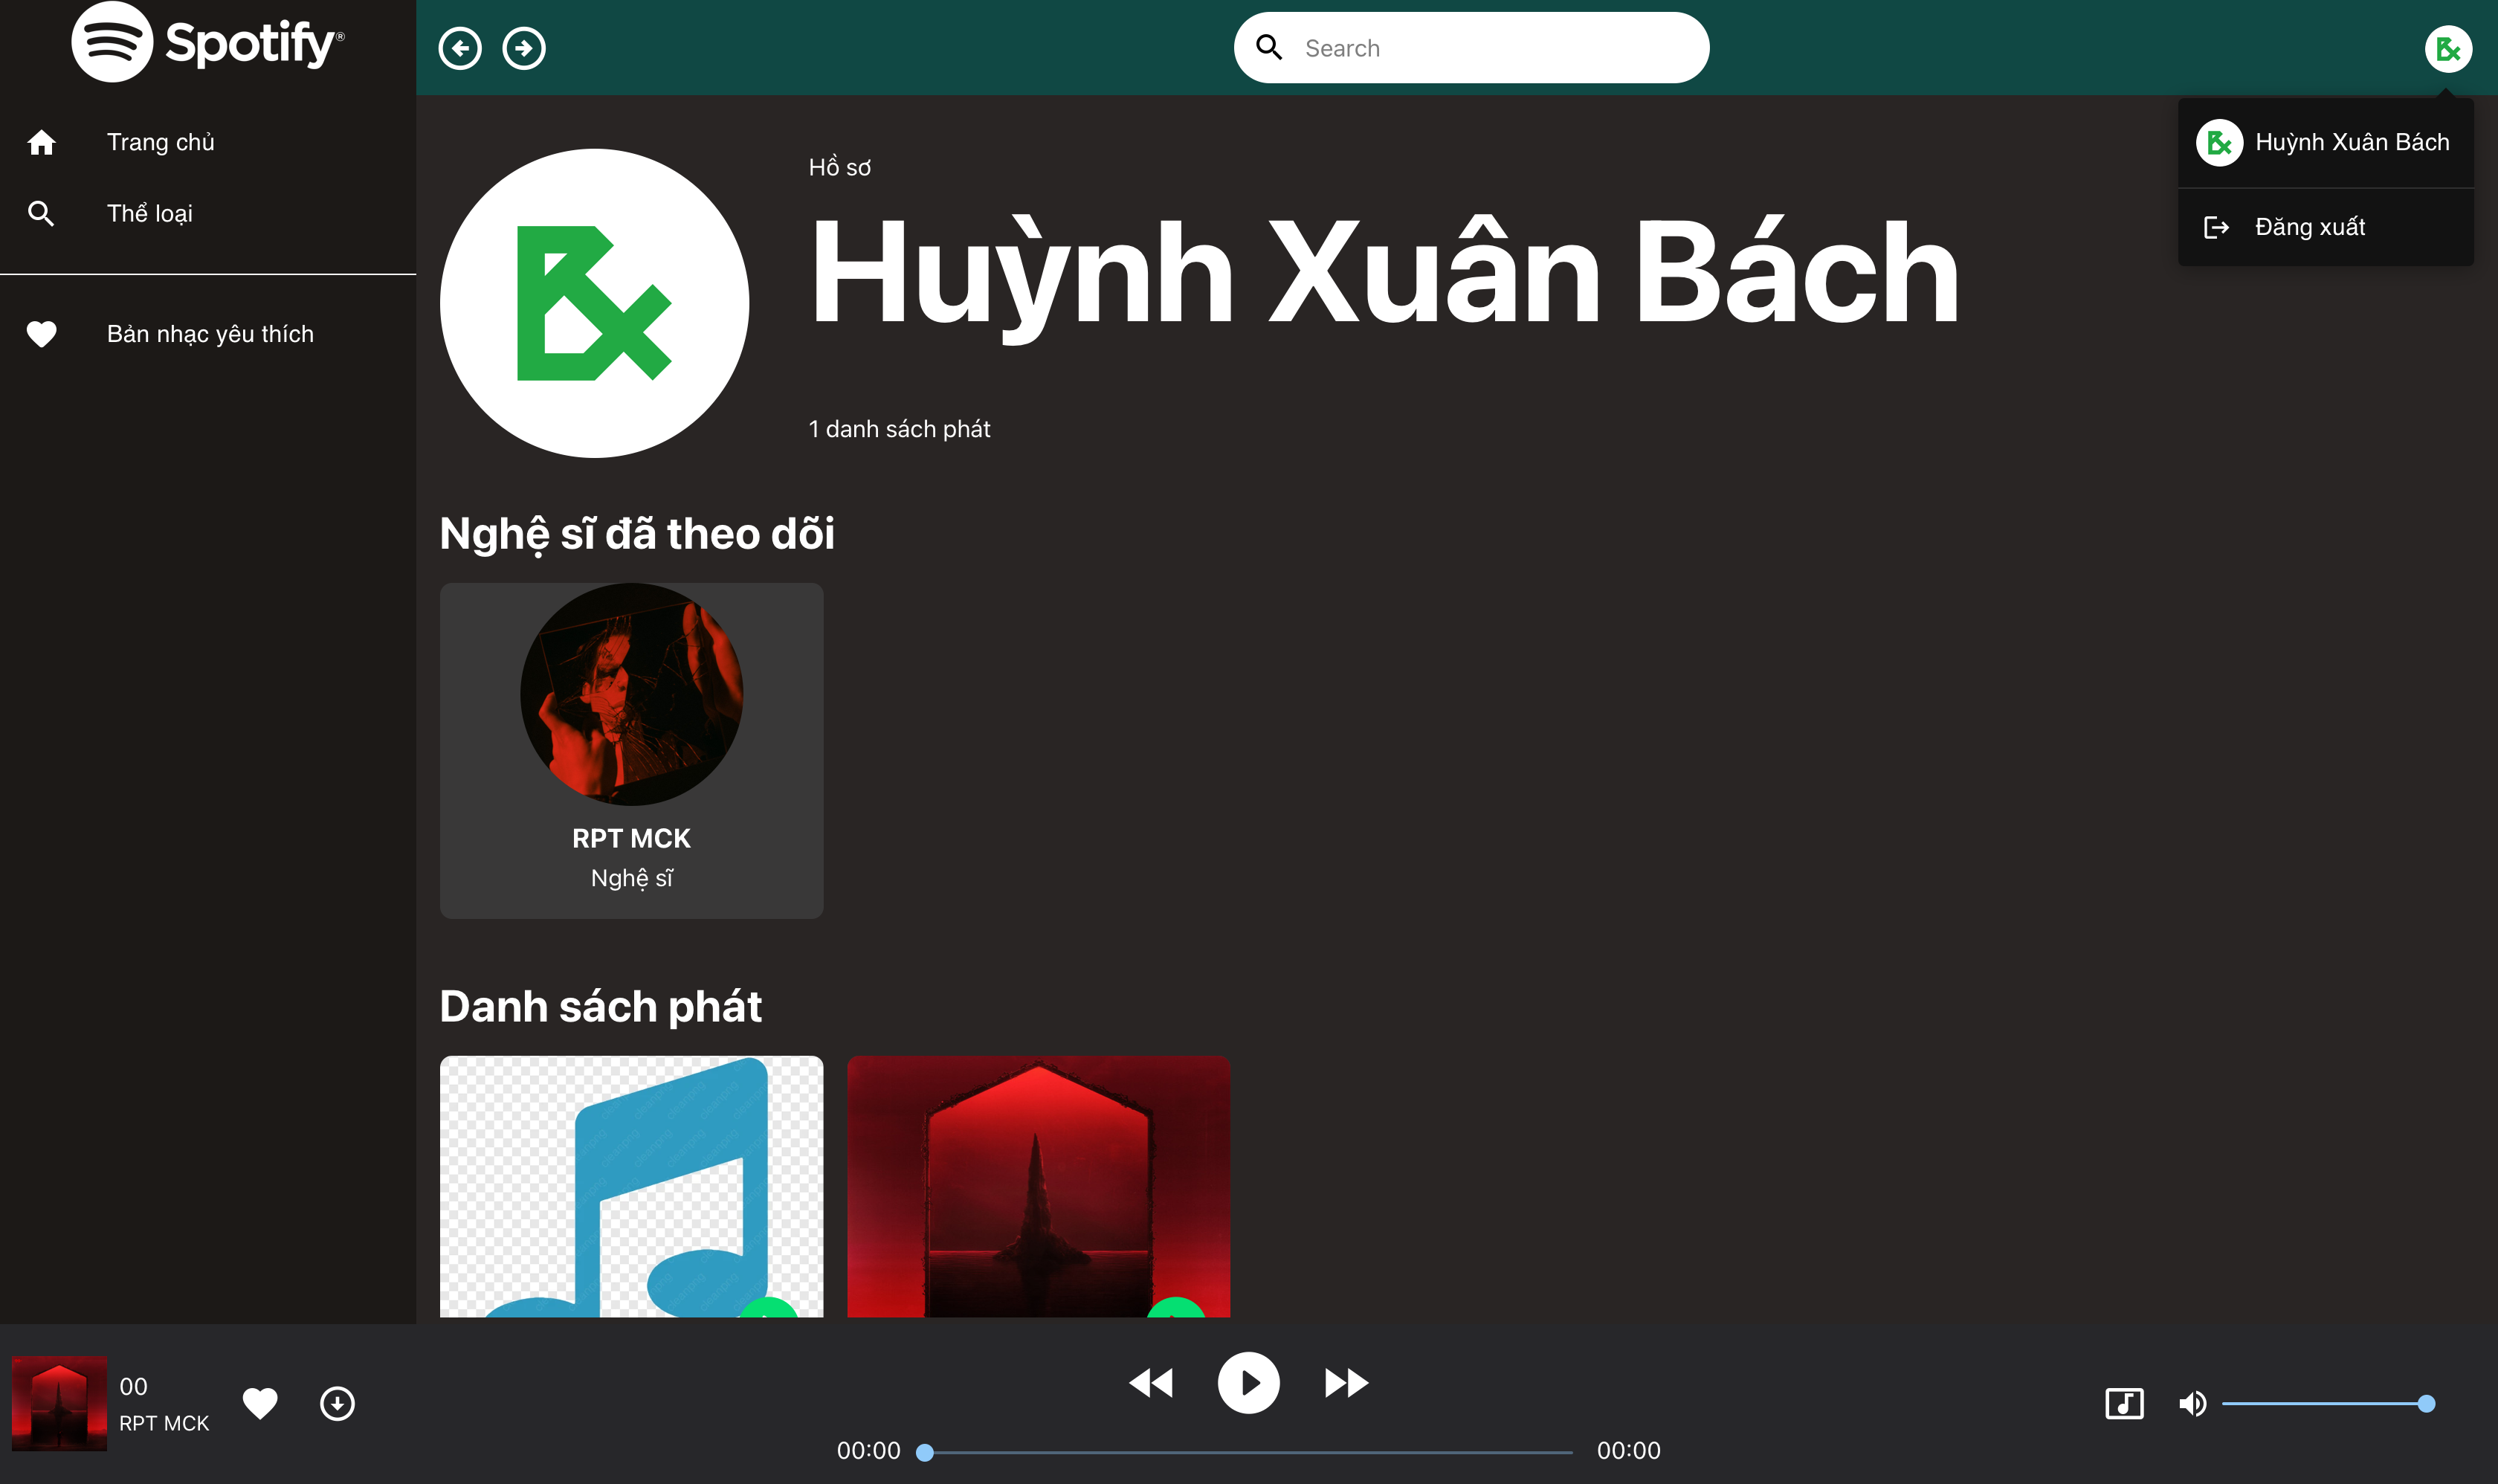
\includegraphics[width=12cm]{profile.png}
\end{center}
\end{figure}

\subsubsection{Tải lên ảnh hồ sơ}
\begin{figure}[h!]
\begin{center}
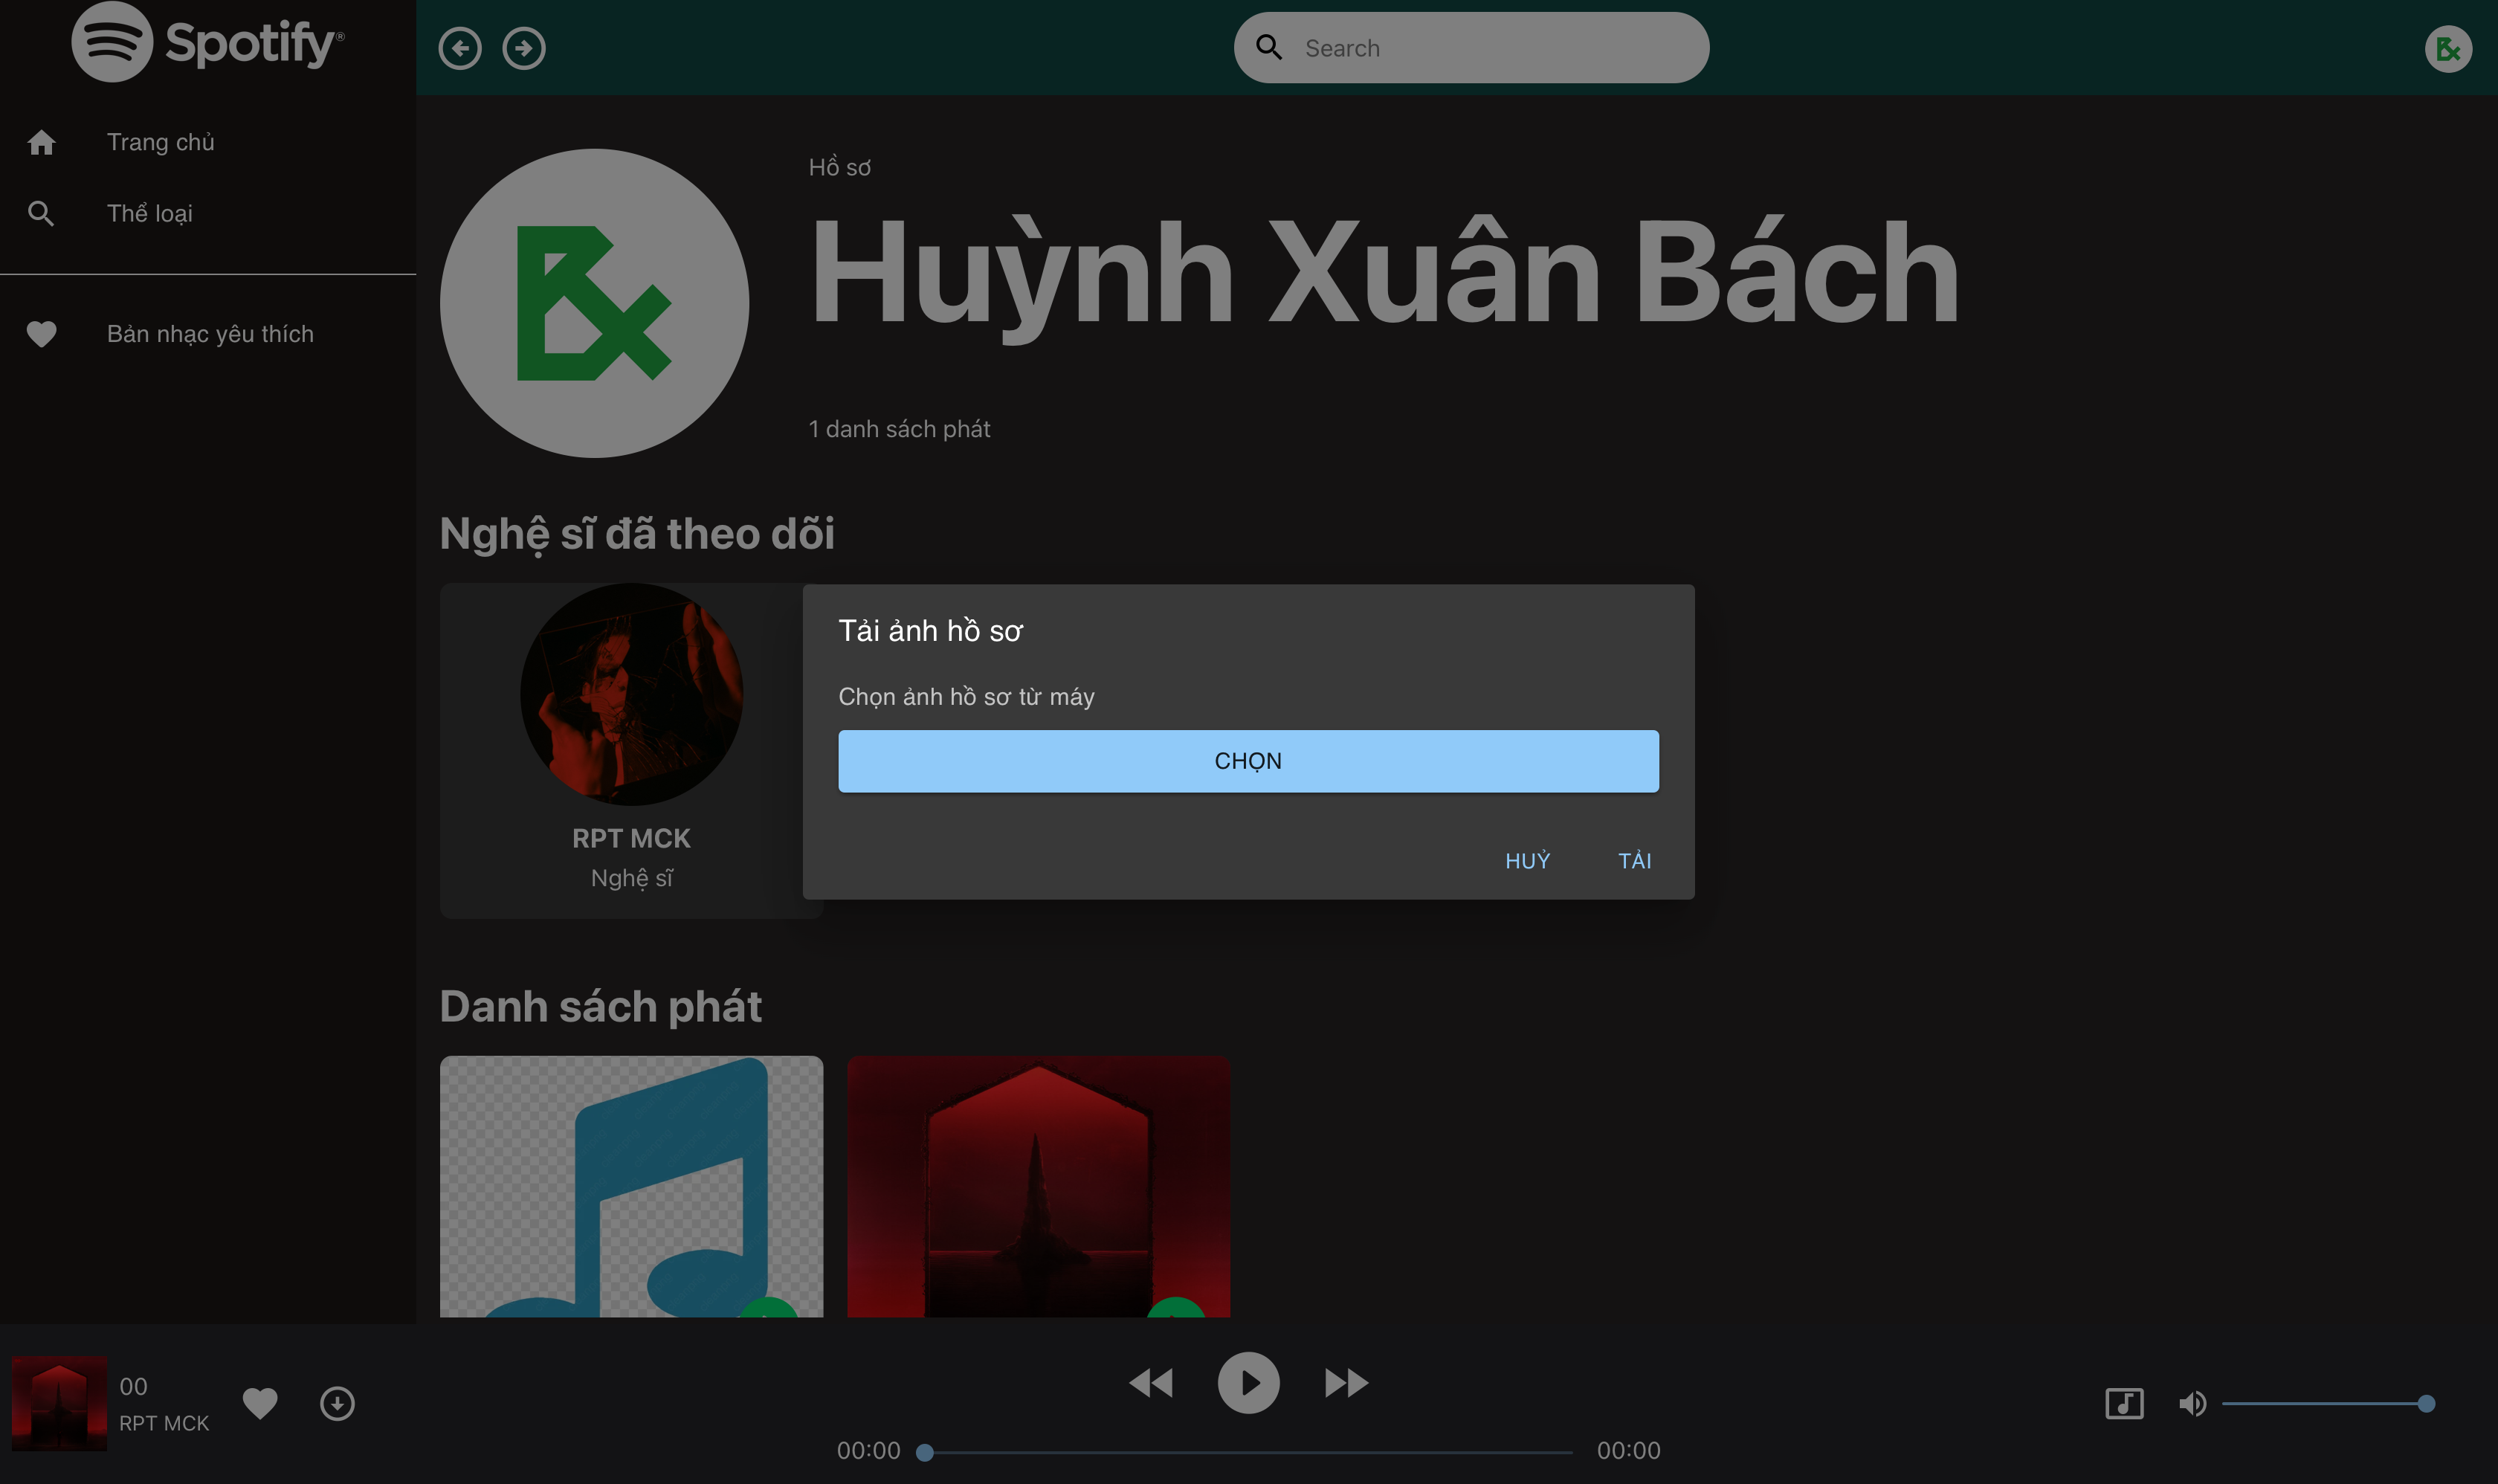
\includegraphics[width=12cm]{profile_image_upload.png}
\end{center}
\end{figure}
\newpage

\subsubsection{Tạo danh sách phát}
\begin{figure}[h!]
\begin{center}
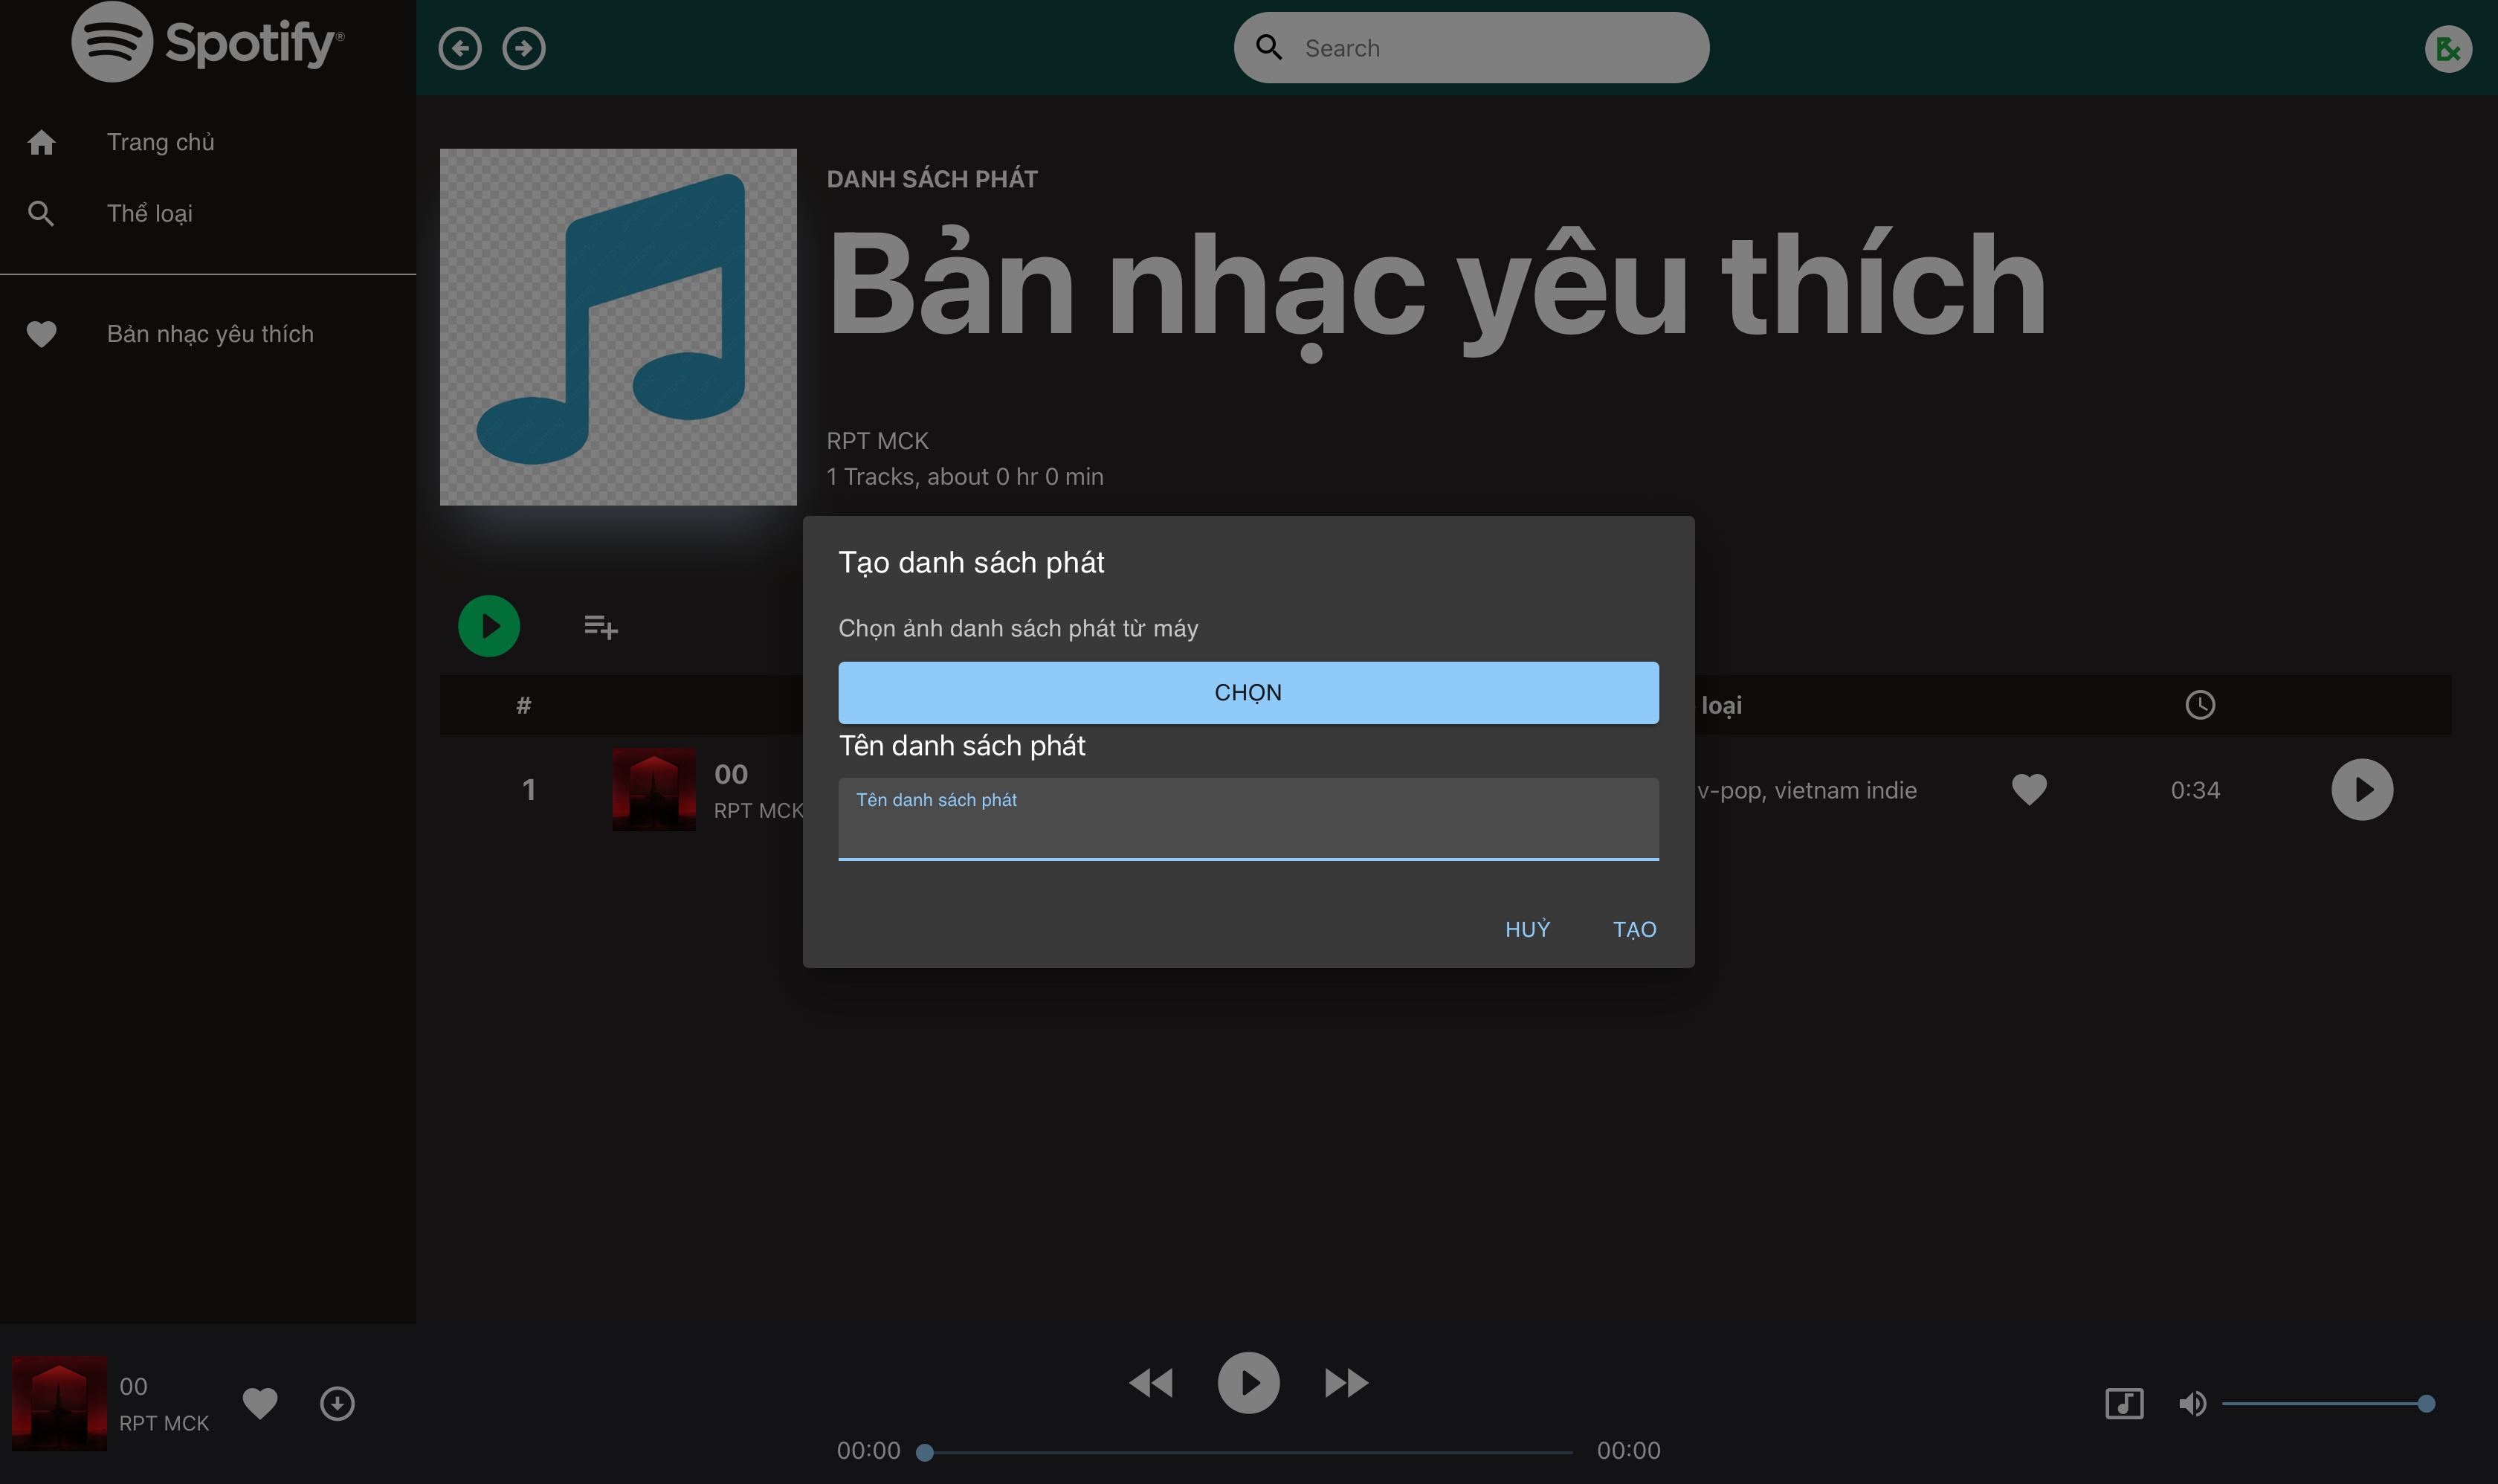
\includegraphics[width=12cm]{playlist_create.png}
\end{center}
\end{figure}

\subsubsection{Xoá danh sách phát}
\begin{figure}[h!]
\begin{center}
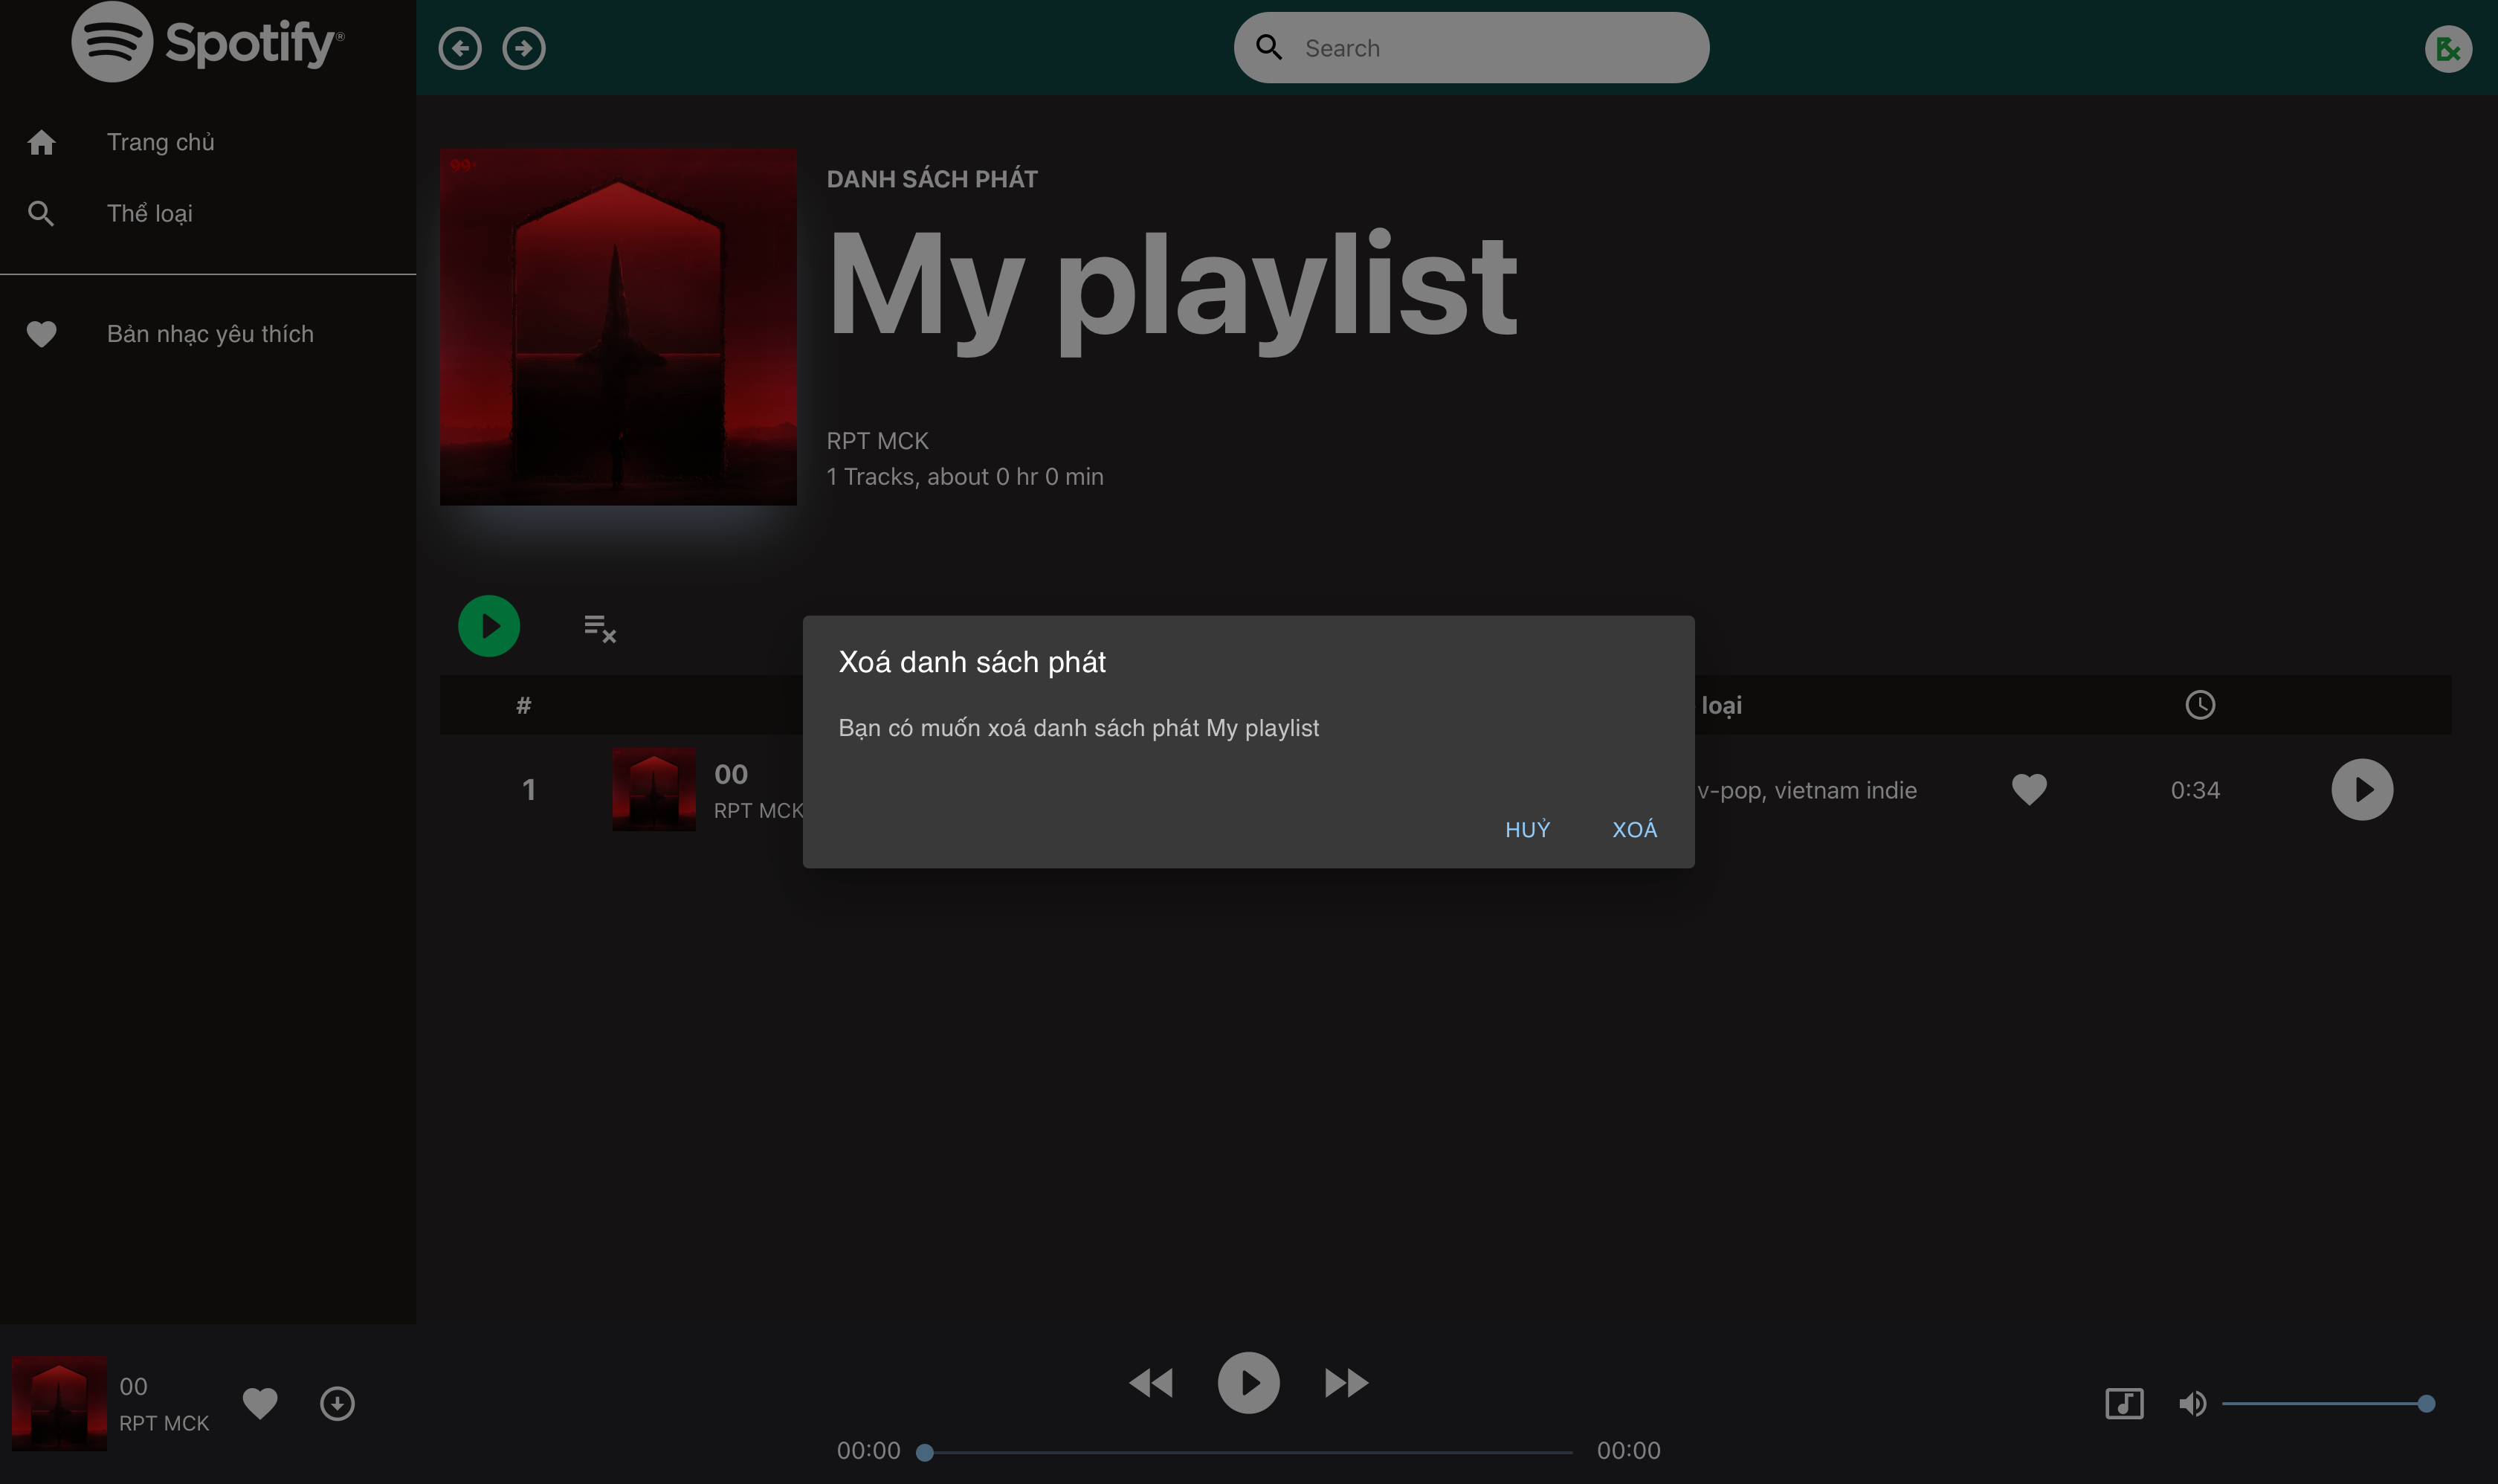
\includegraphics[width=12cm]{playlist_delete.png}
\end{center}
\end{figure}
\newpage

\subsubsection{Đăng nhập}
\begin{figure}[h!]
\begin{center}
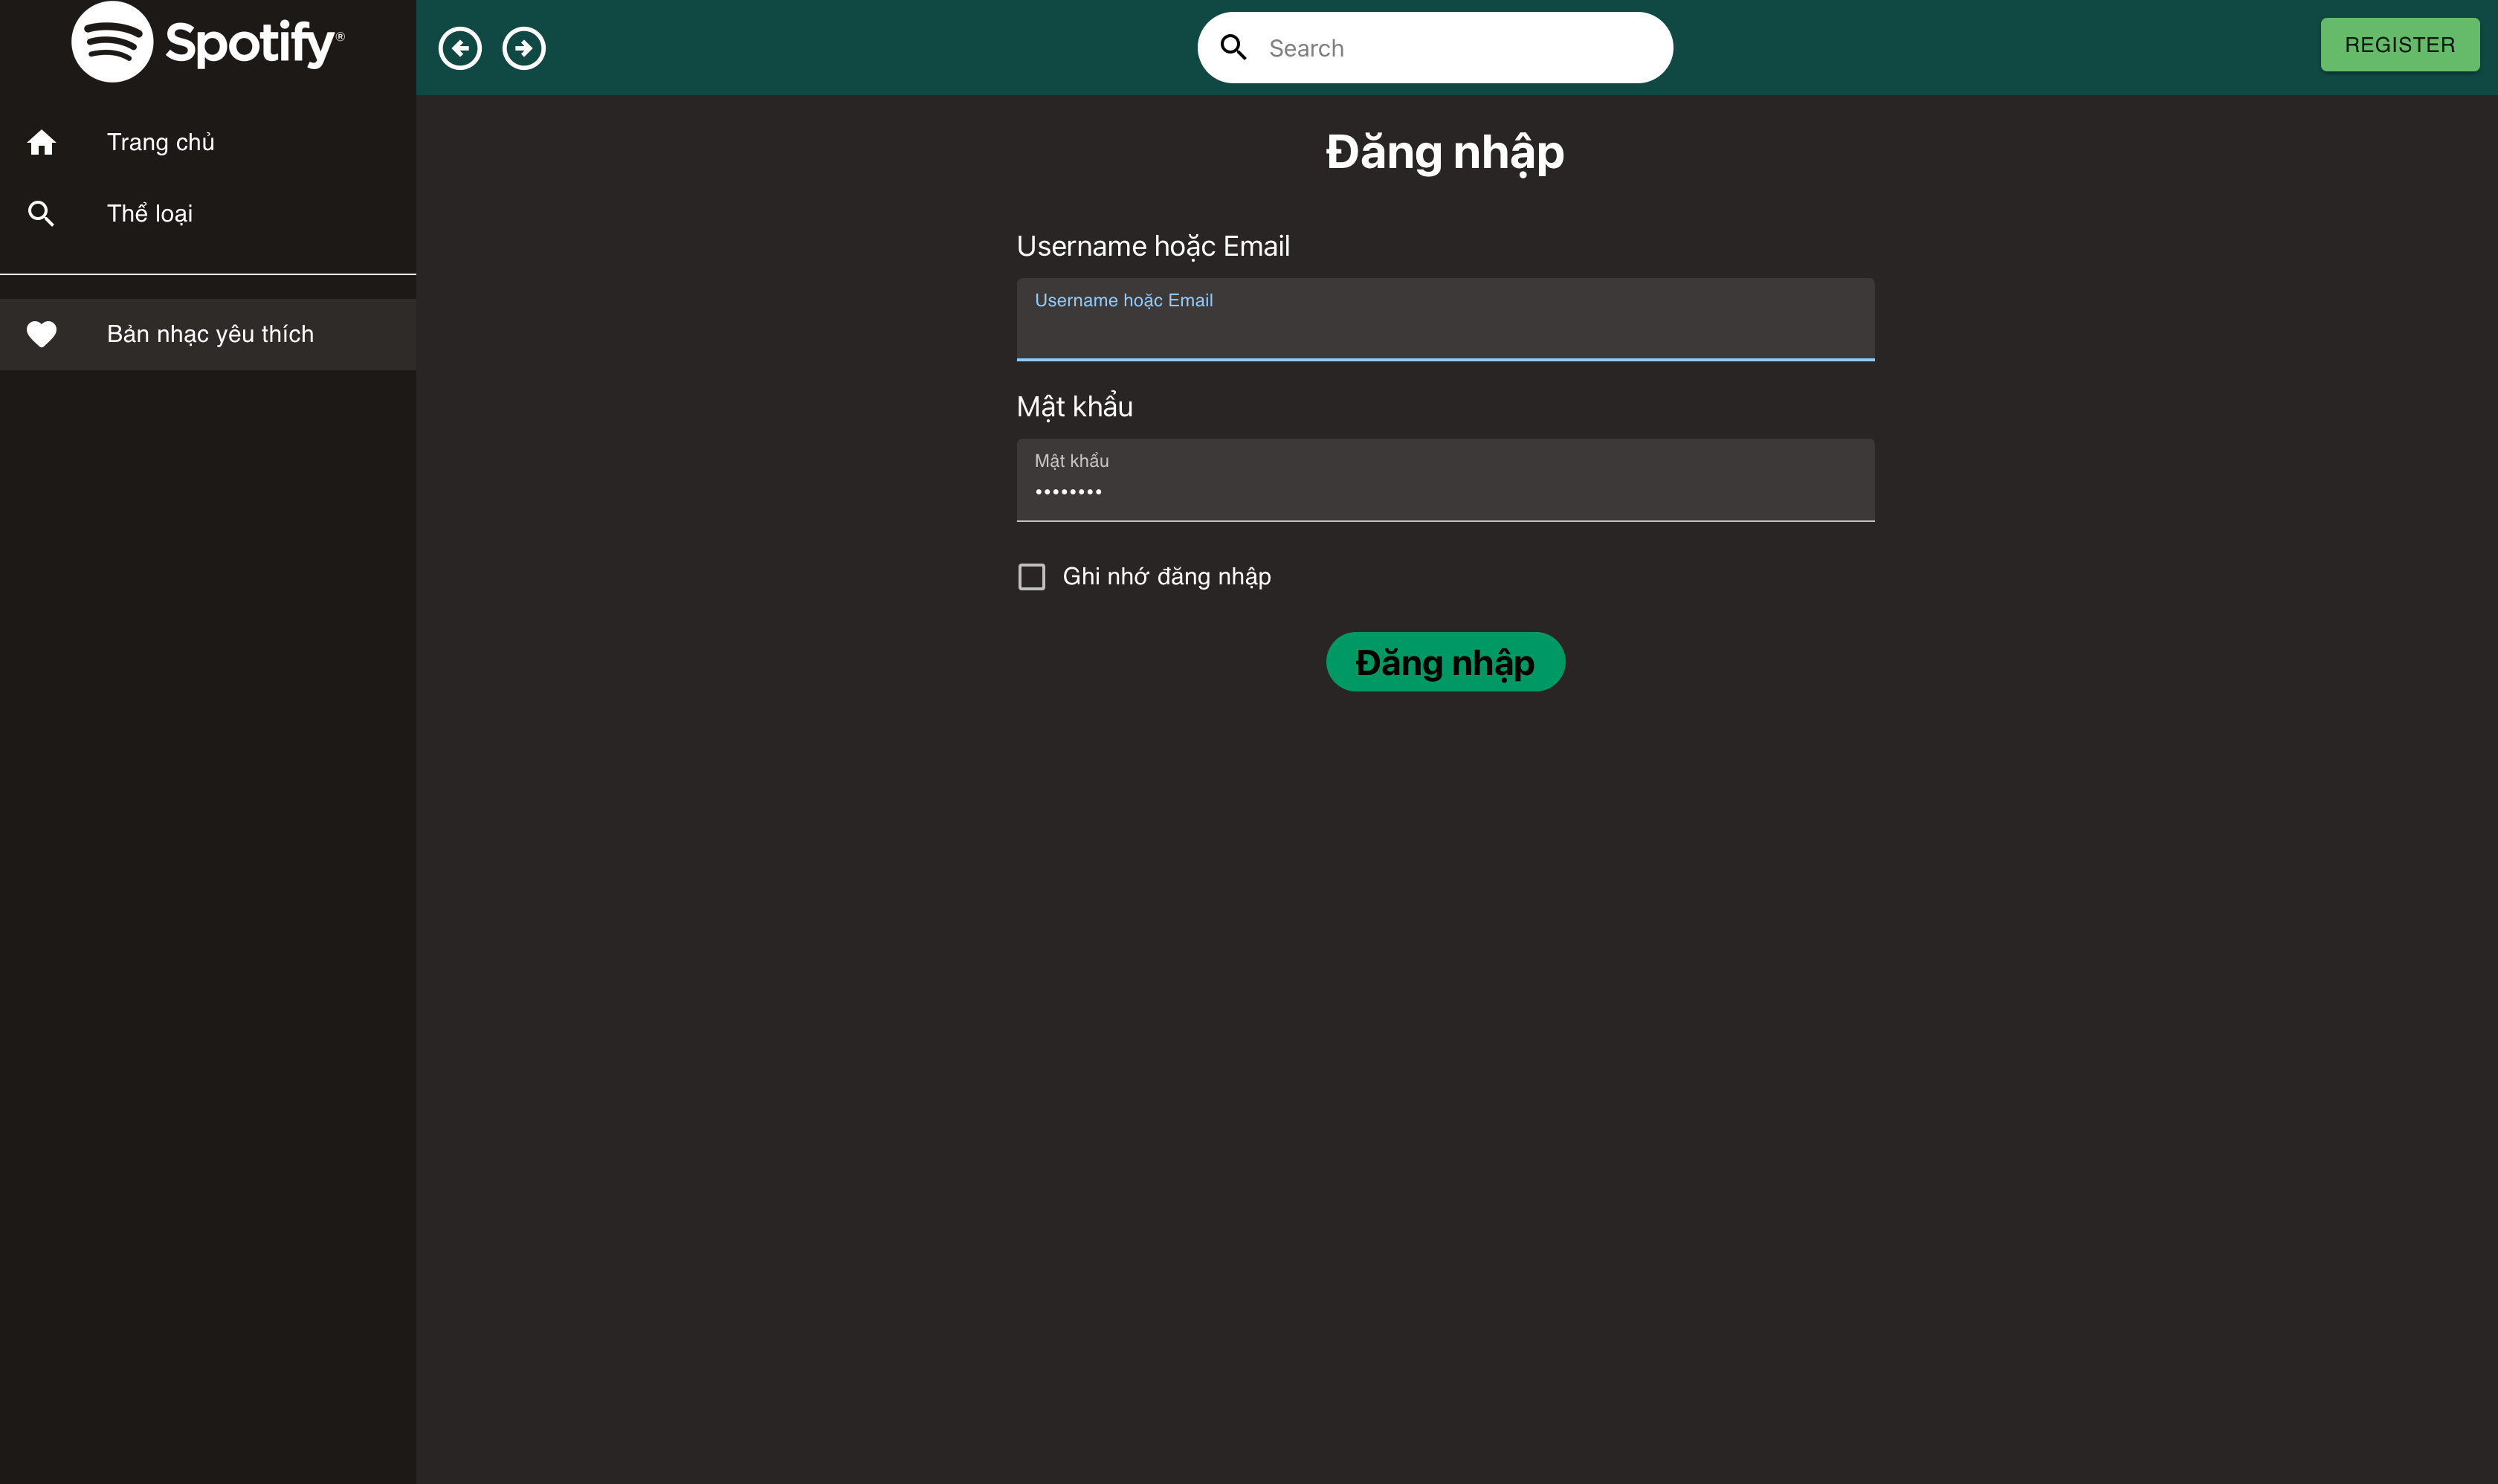
\includegraphics[width=12cm]{login.png}
\end{center}
\end{figure}

\subsubsection{Đăng ký}
\begin{figure}[h!]
\begin{center}
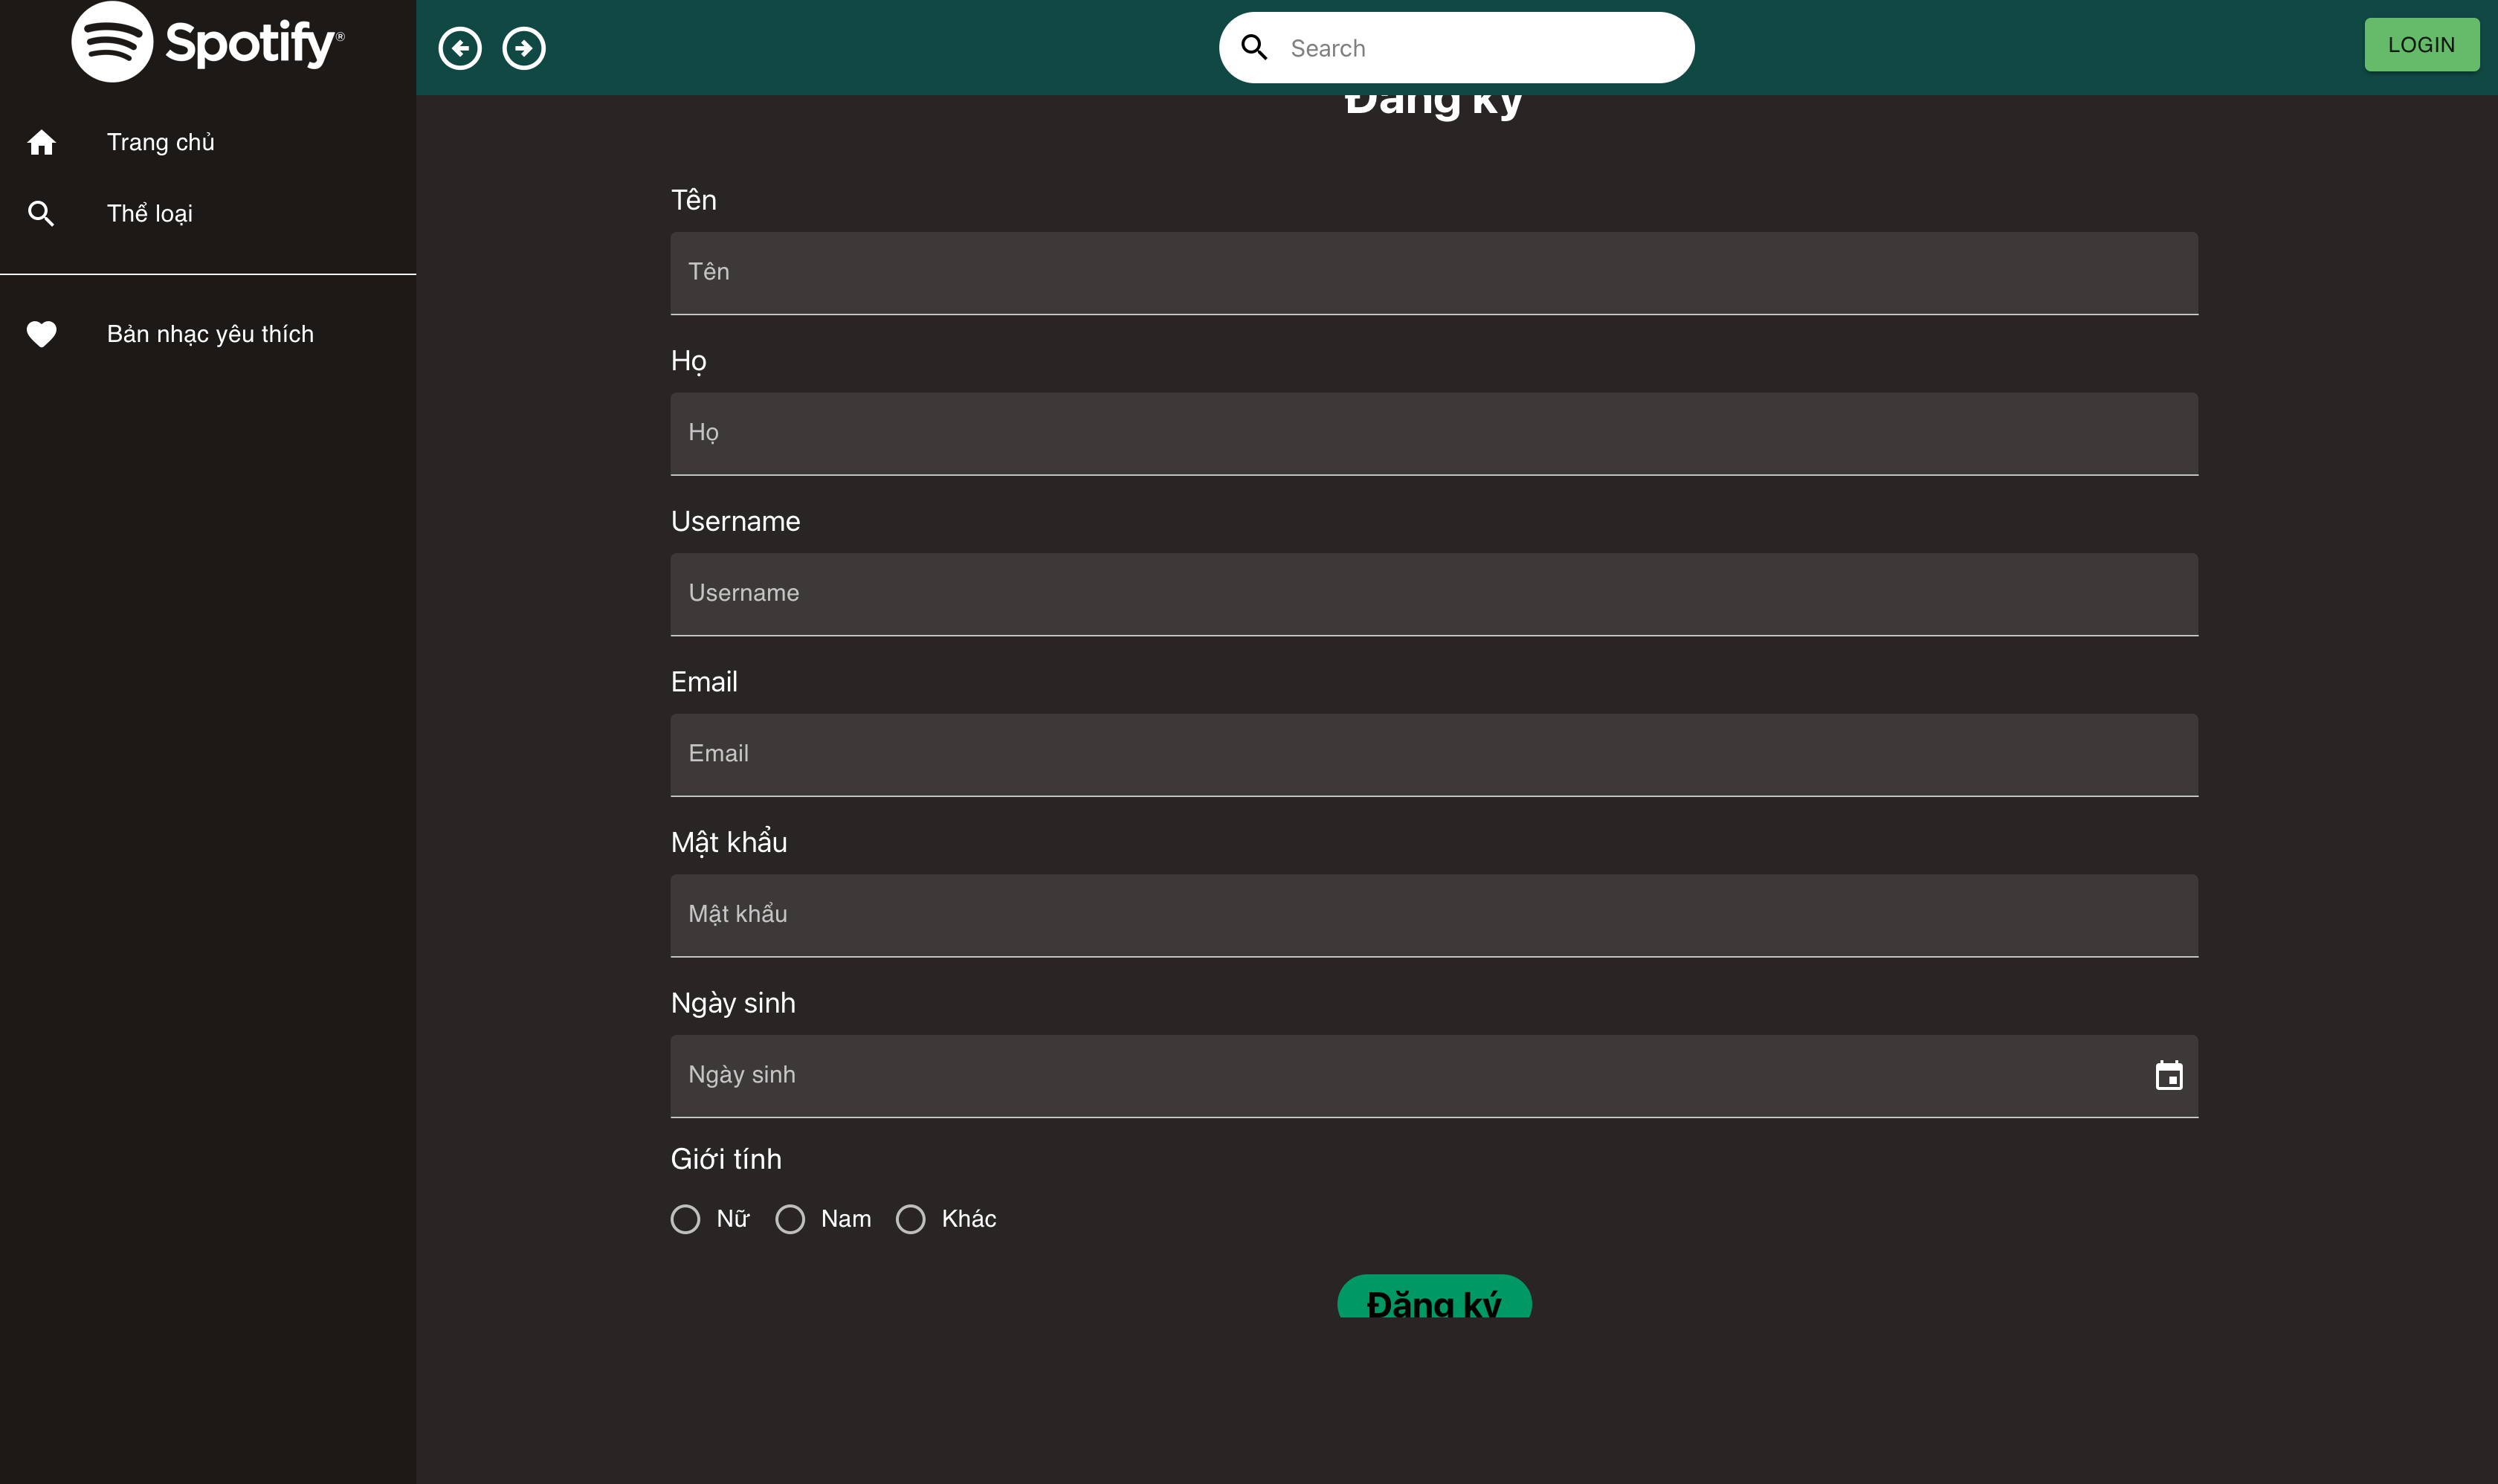
\includegraphics[width=12cm]{register.png}
\end{center}
\end{figure}
\newpage

\subsubsection{Trang admin - Hồ sơ}
\begin{figure}[h!]
\begin{center}
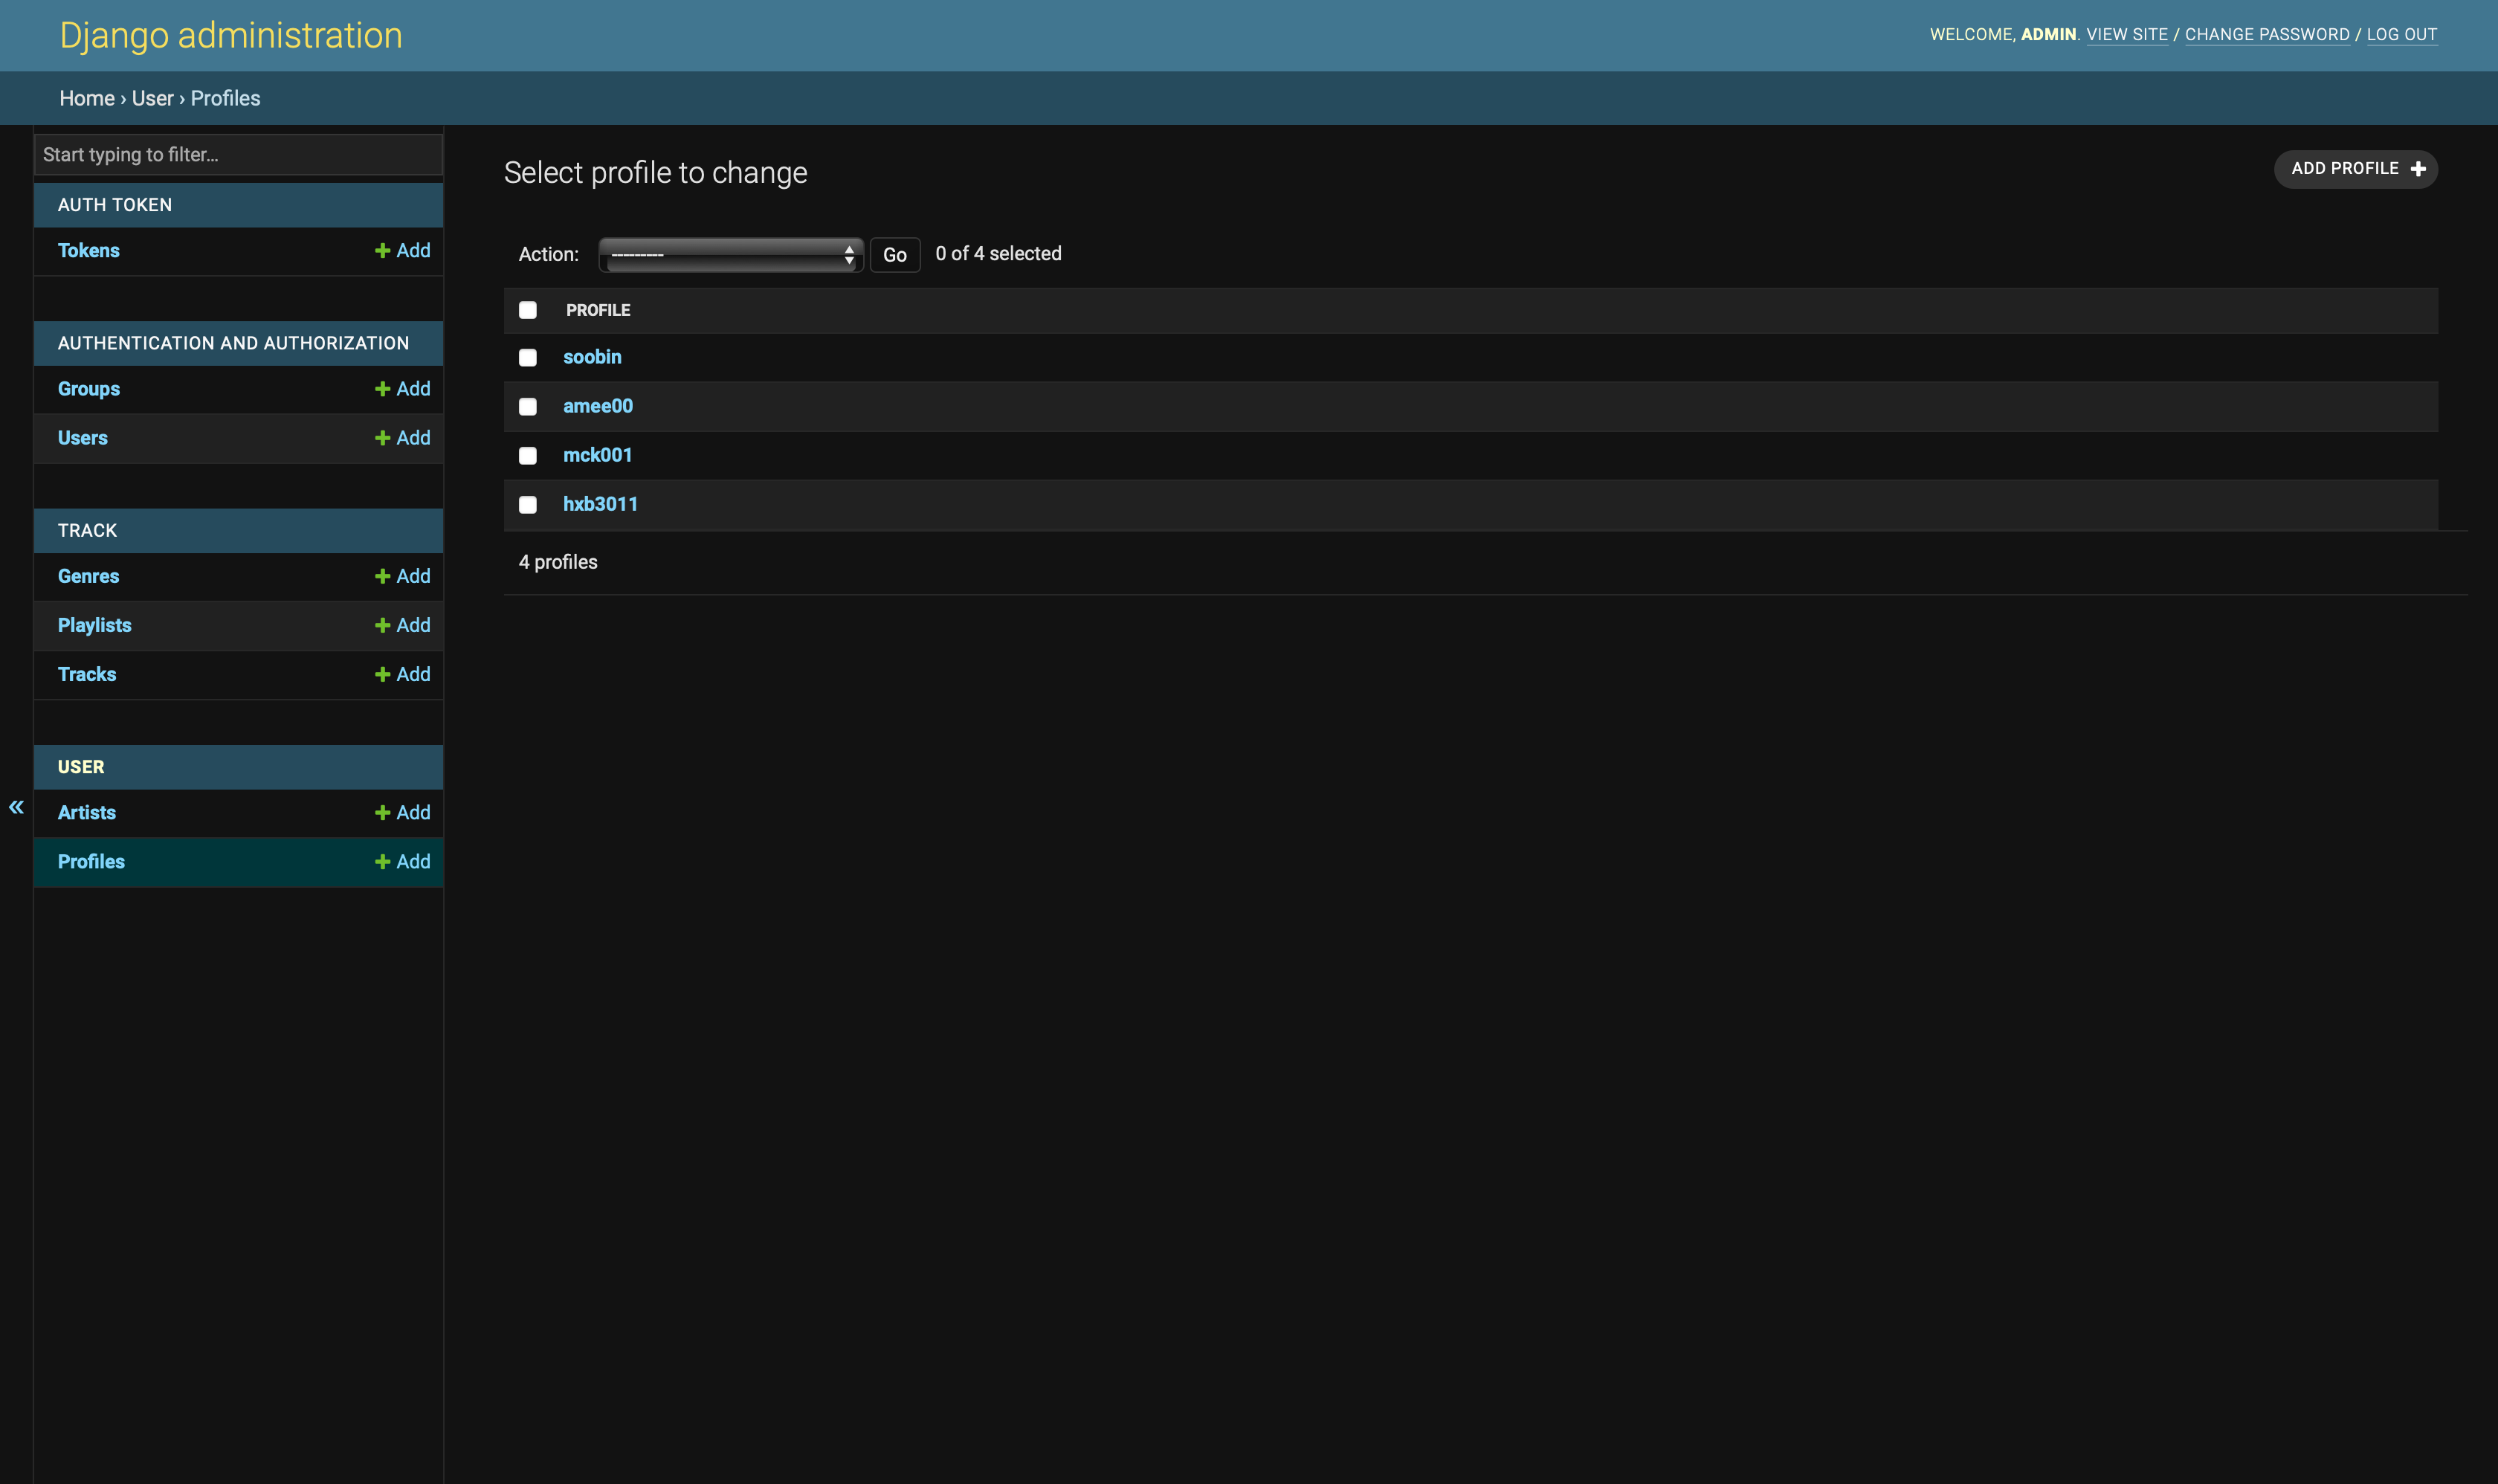
\includegraphics[width=12cm]{admin_profile.png}
\end{center}
\end{figure}

\subsubsection{Trang admin - Chi tiết hồ sơ}
\begin{figure}[h!]
\begin{center}
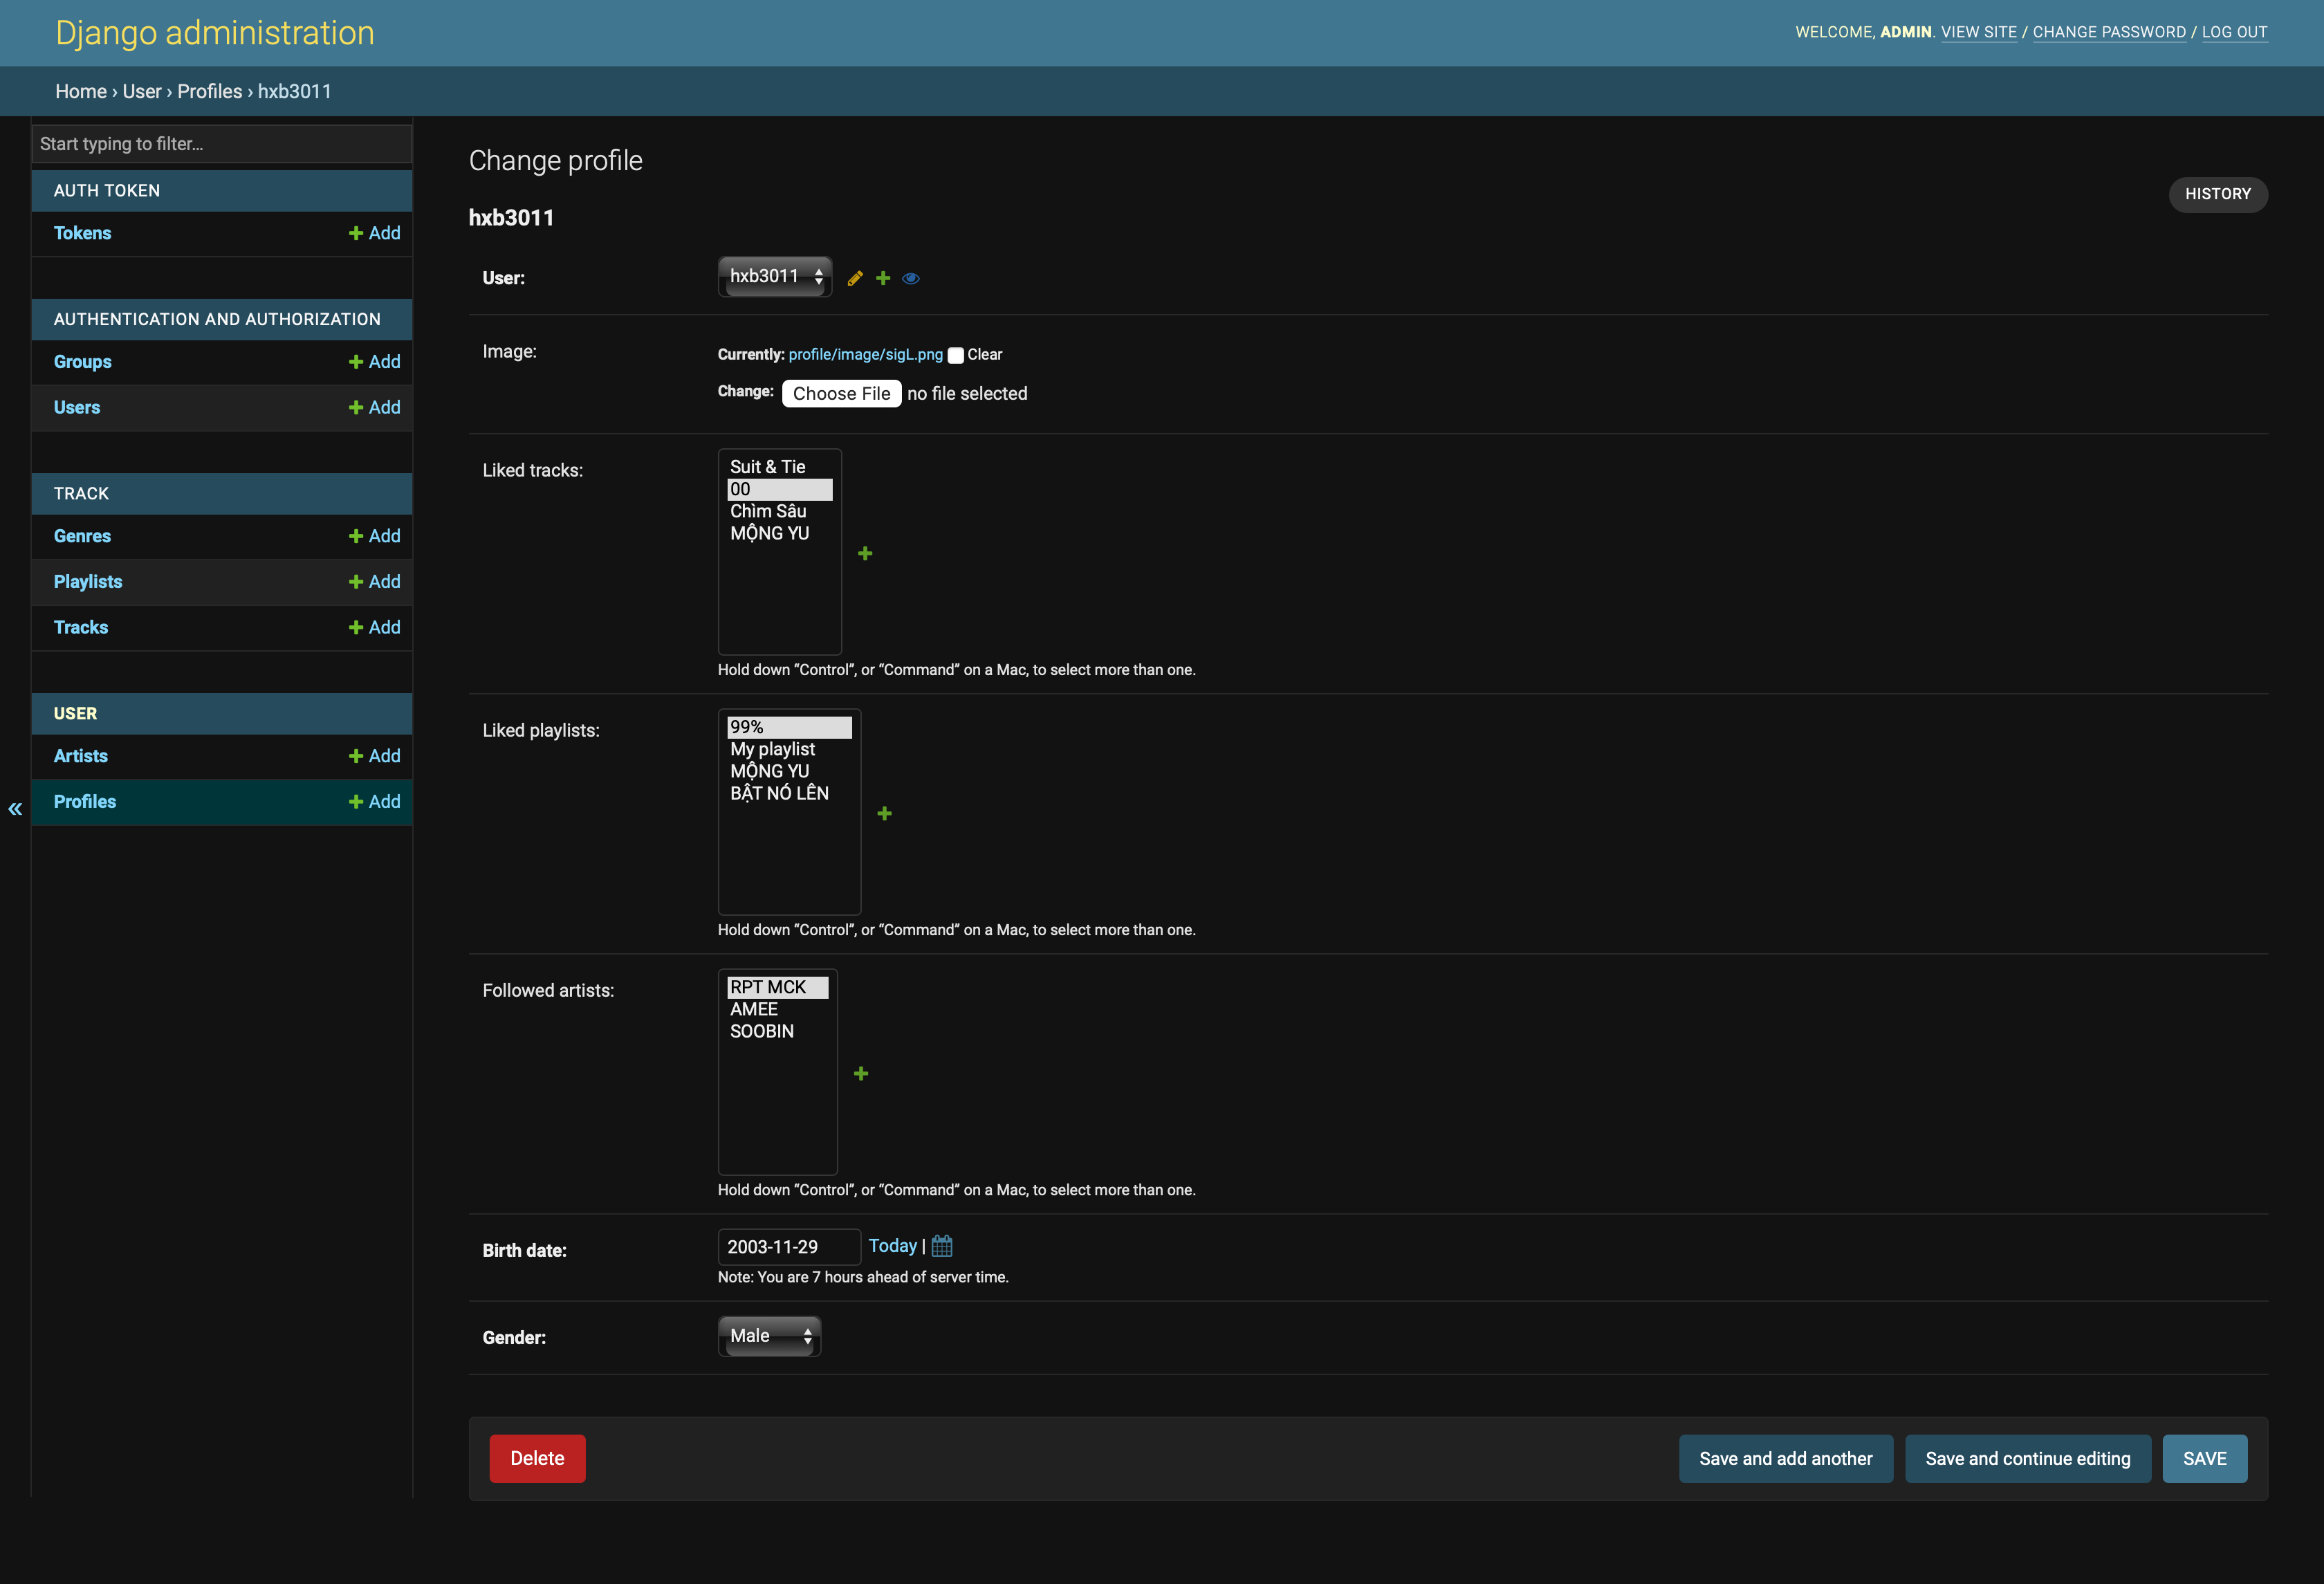
\includegraphics[width=12cm]{admin_profile_detail.png}
\end{center}
\end{figure}
\newpage

\subsubsection{Trang admin - Nghệ sĩ}
\begin{figure}[h!]
\begin{center}
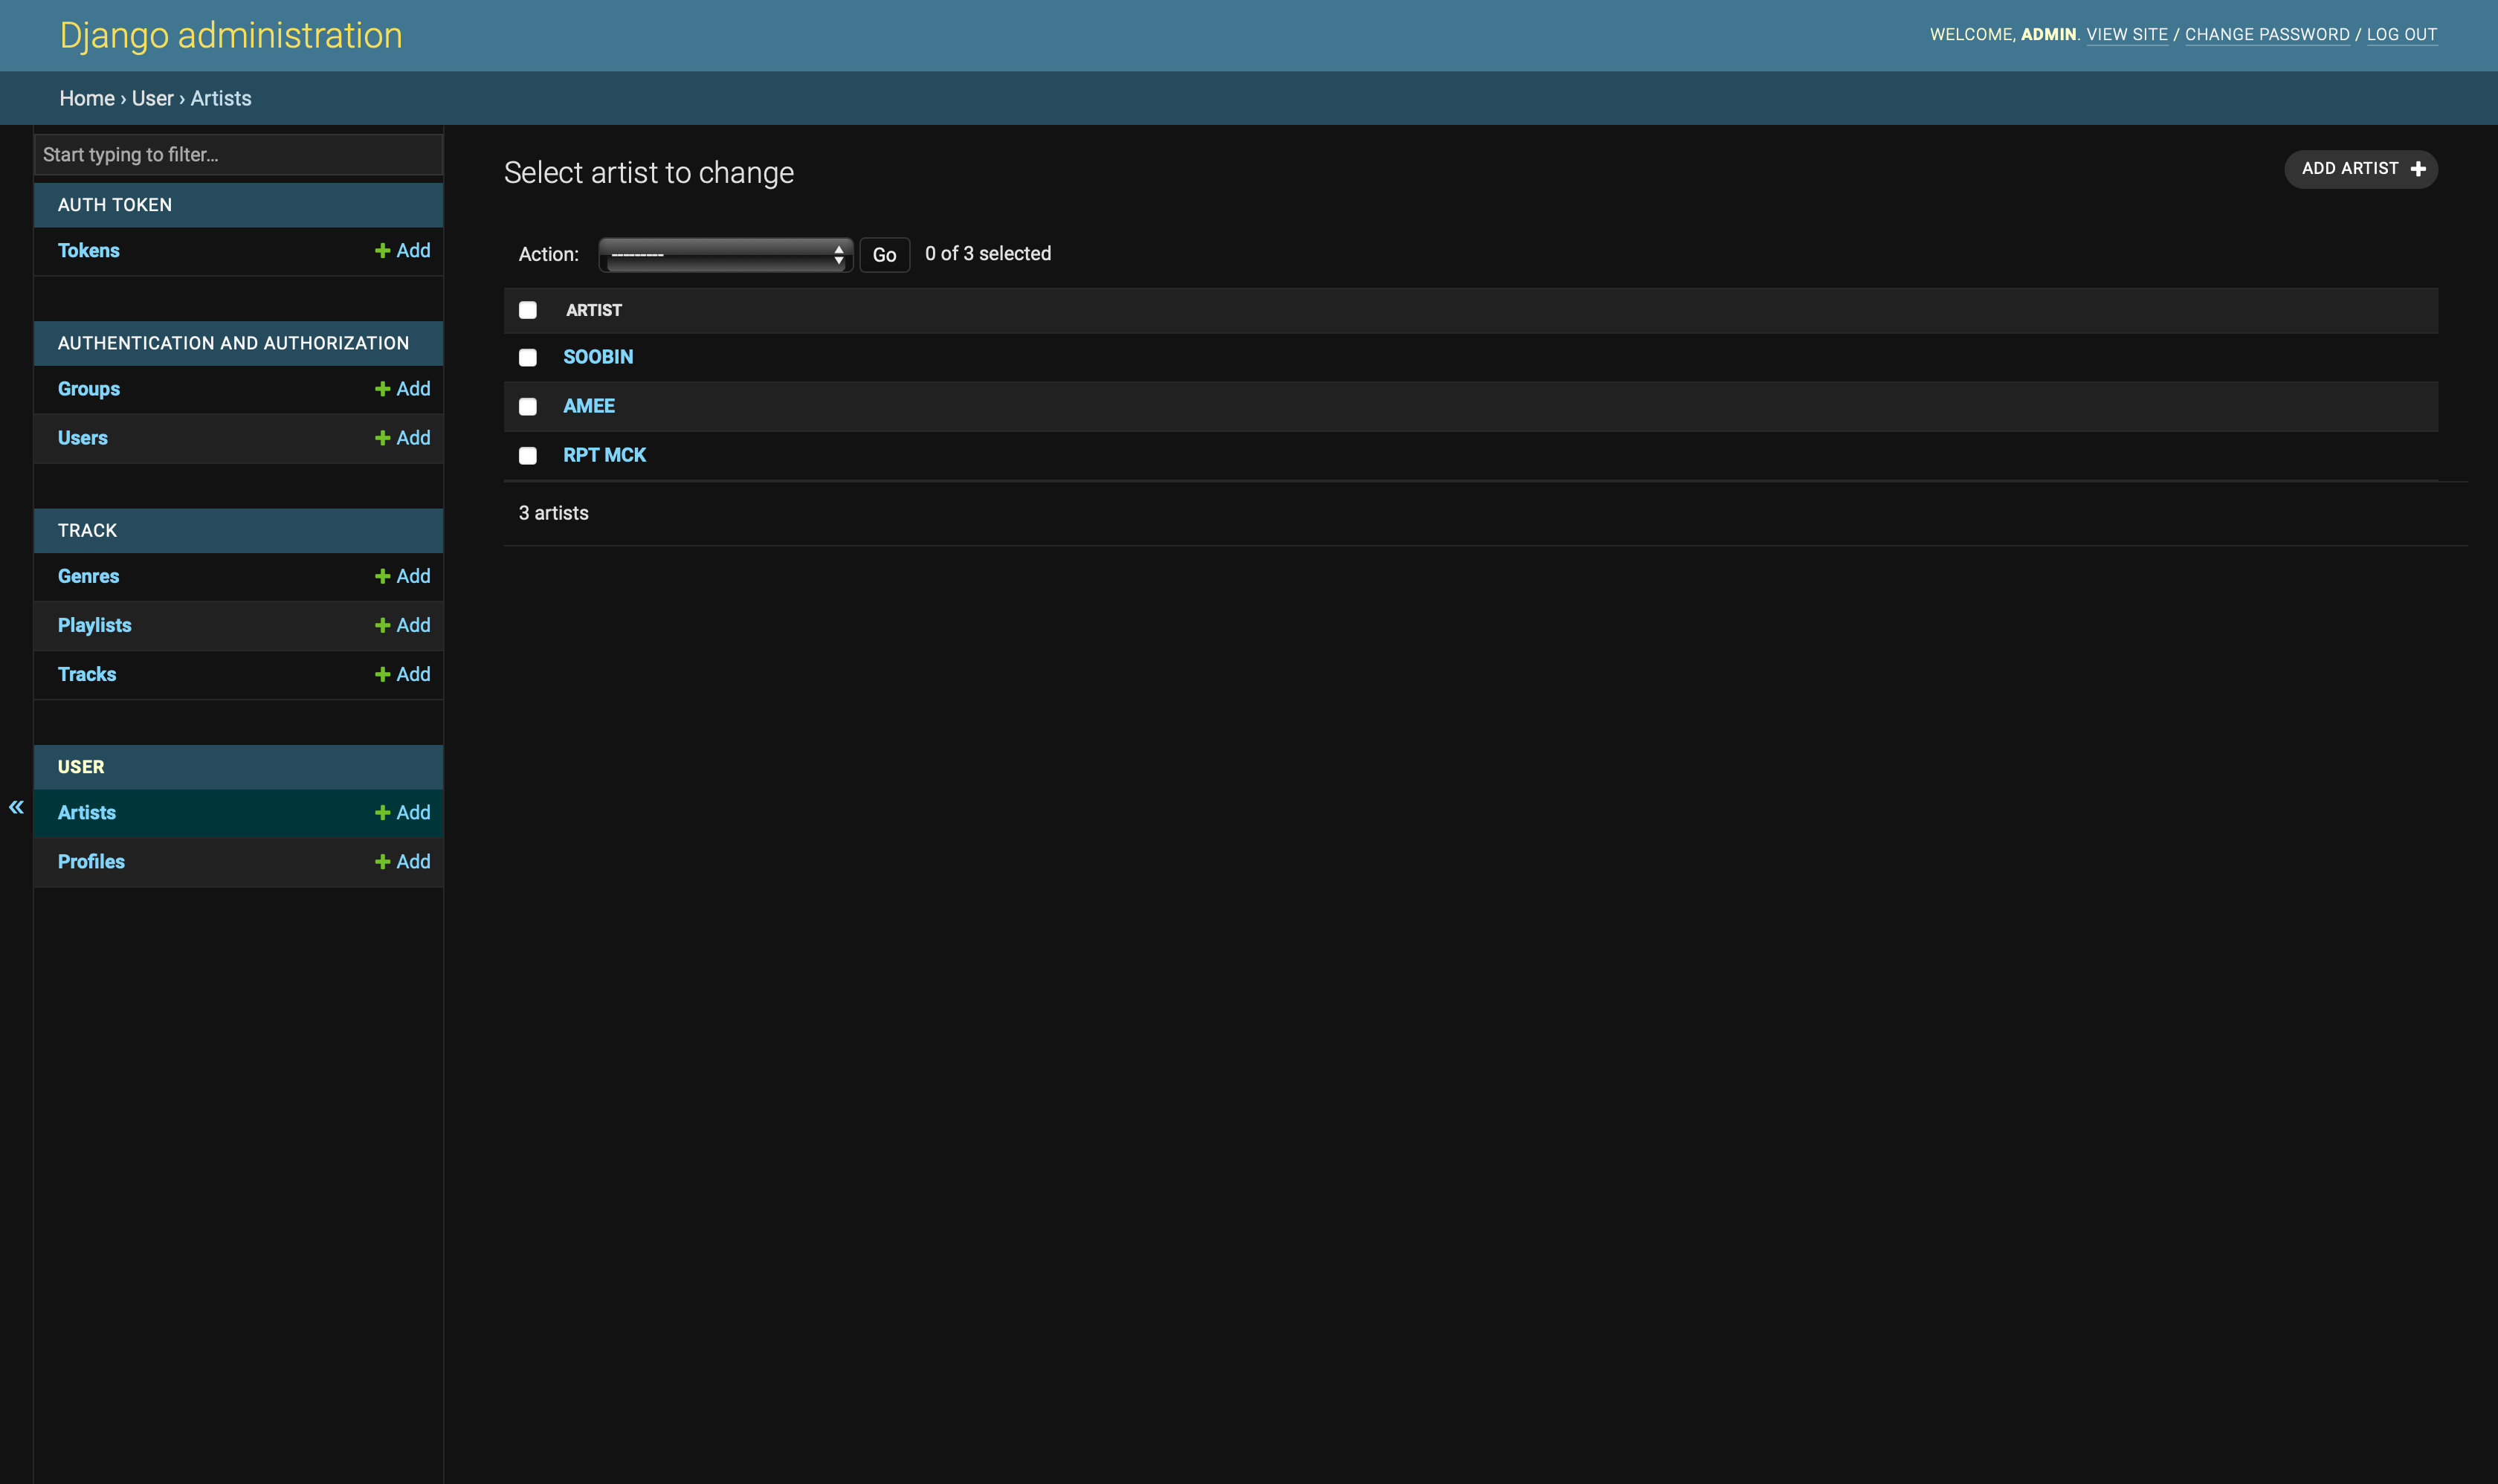
\includegraphics[width=12cm]{admin_artist.png}
\end{center}
\end{figure}

\subsubsection{Trang admin - Chi tiết nghệ sĩ}
\begin{figure}[h!]
\begin{center}
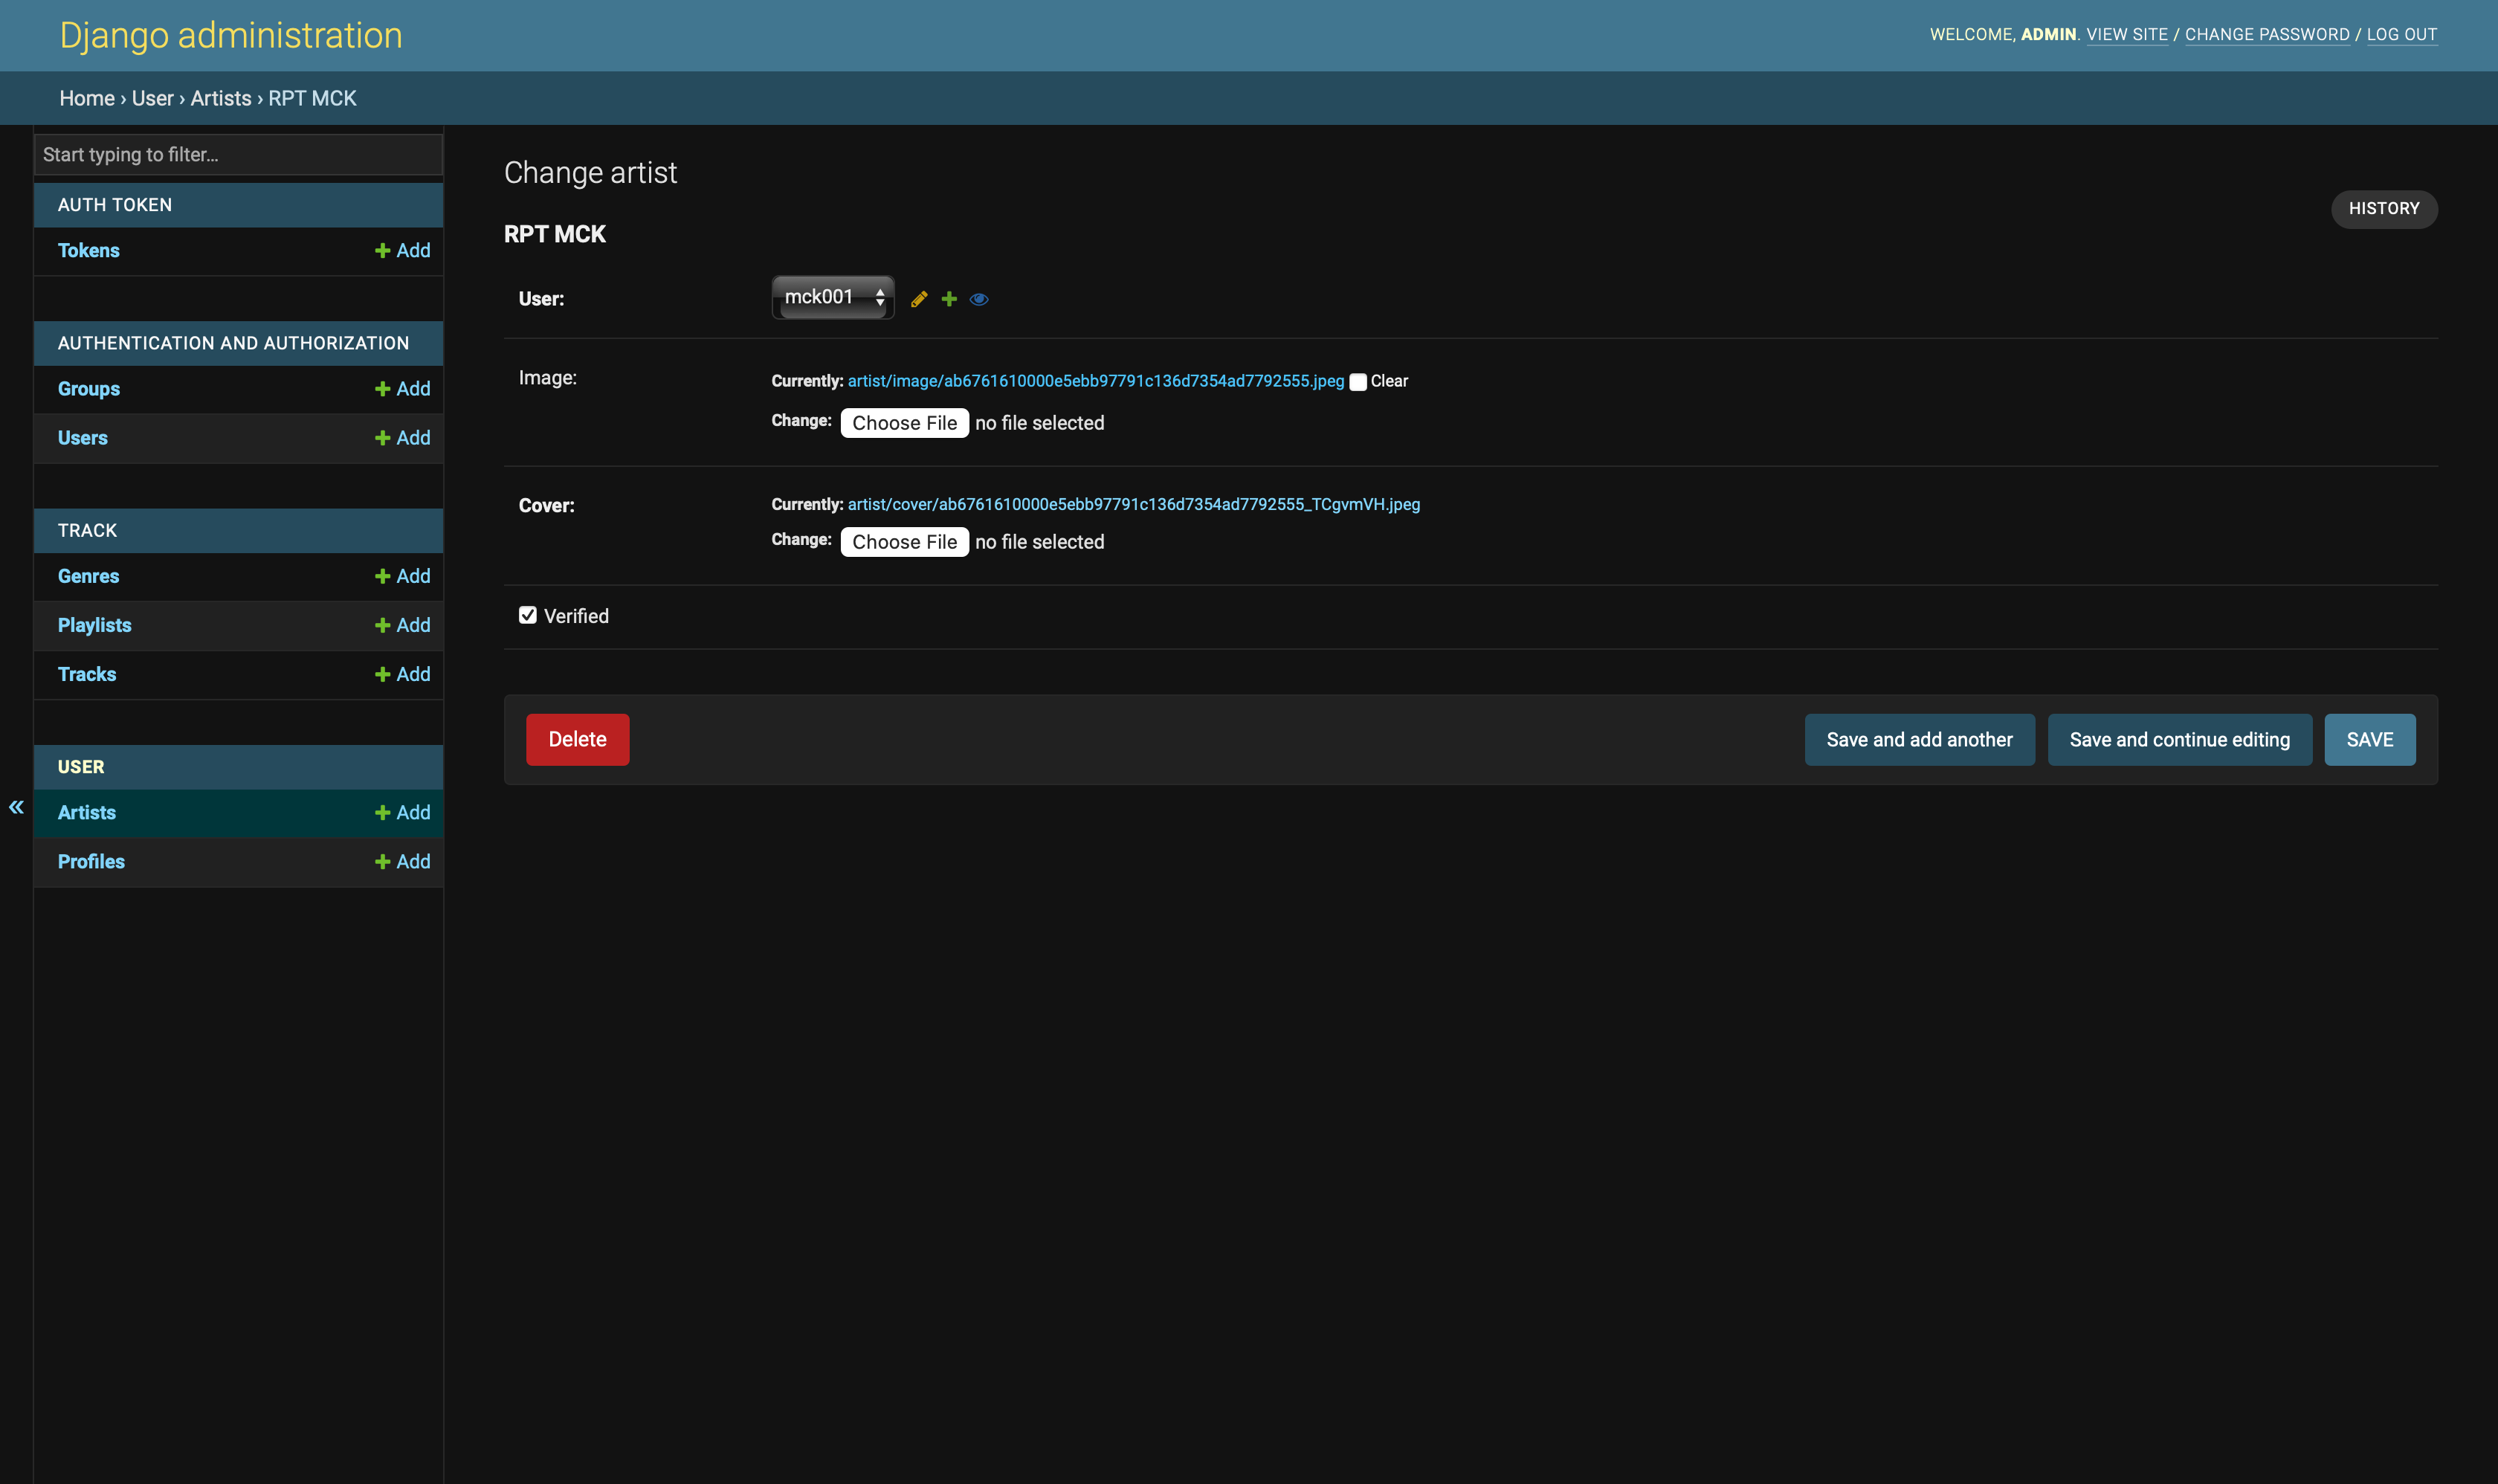
\includegraphics[width=12cm]{admin_artist_detail.png}
\end{center}
\end{figure}
\newpage

\subsubsection{Trang admin - Thể loại}
\begin{figure}[h!]
\begin{center}
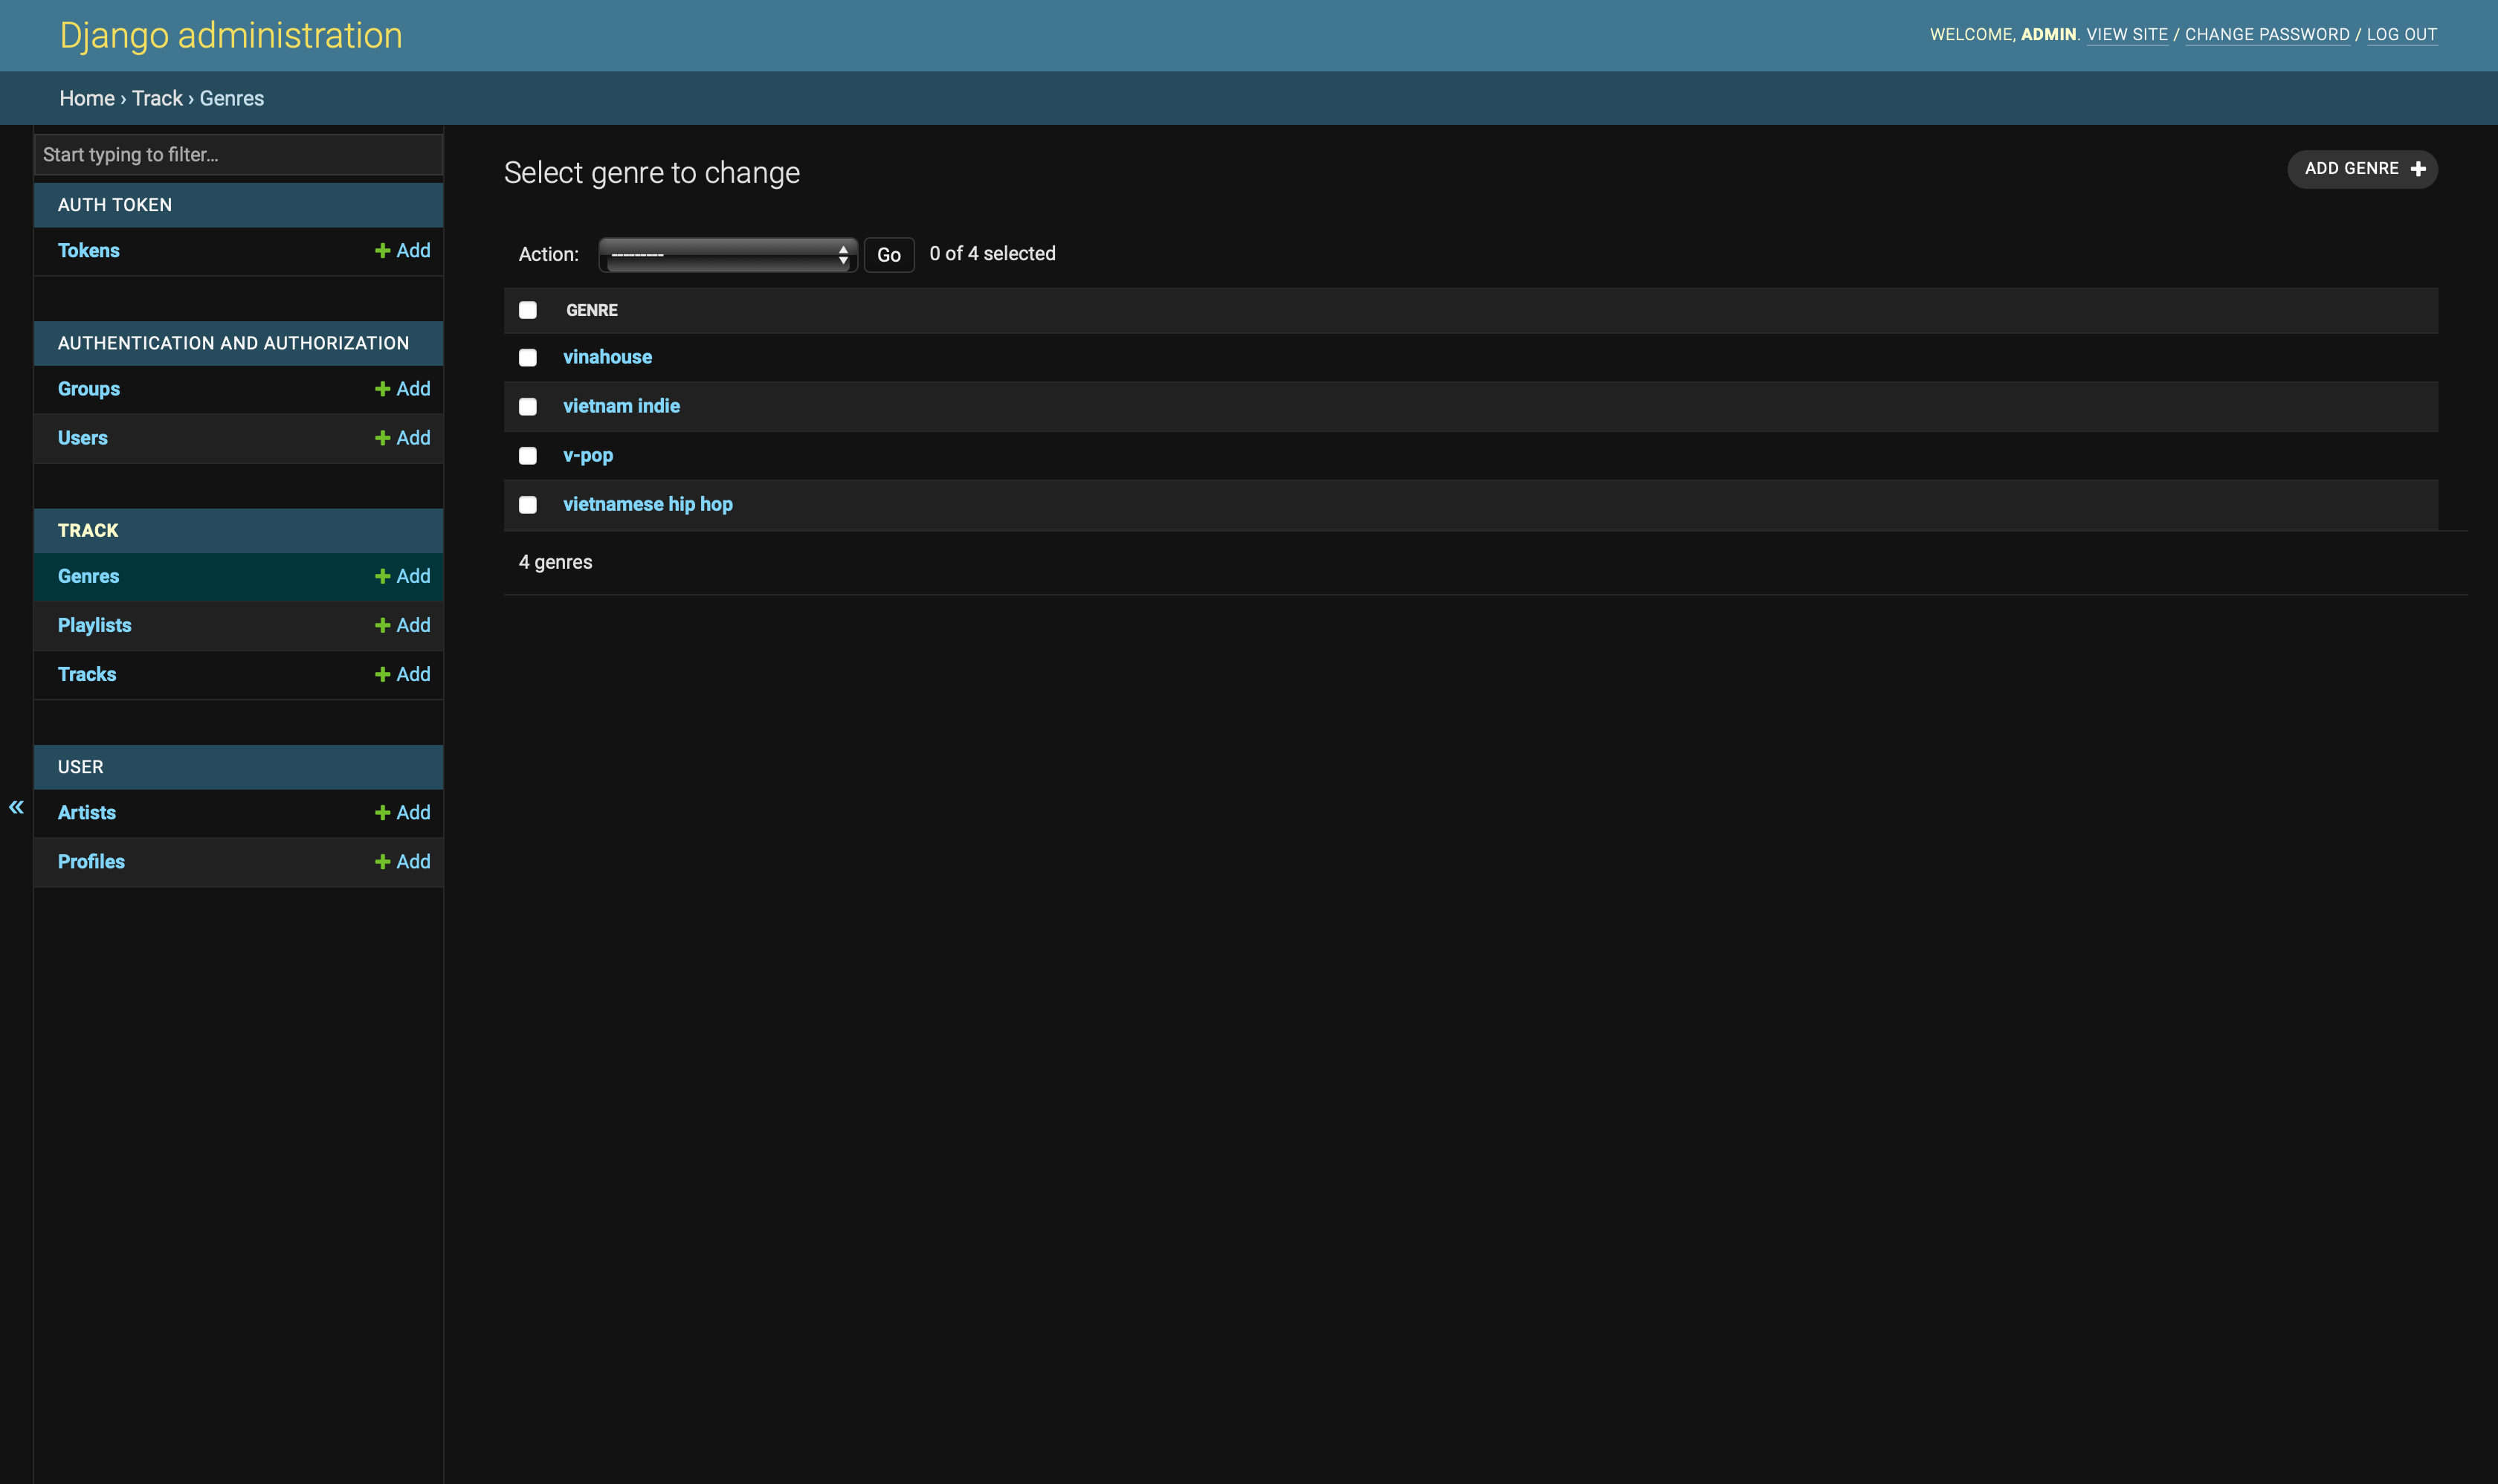
\includegraphics[width=12cm]{admin_genres.png}
\end{center}
\end{figure}

\subsubsection{Trang admin - Chi tiết thể loại}
\begin{figure}[h!]
\begin{center}
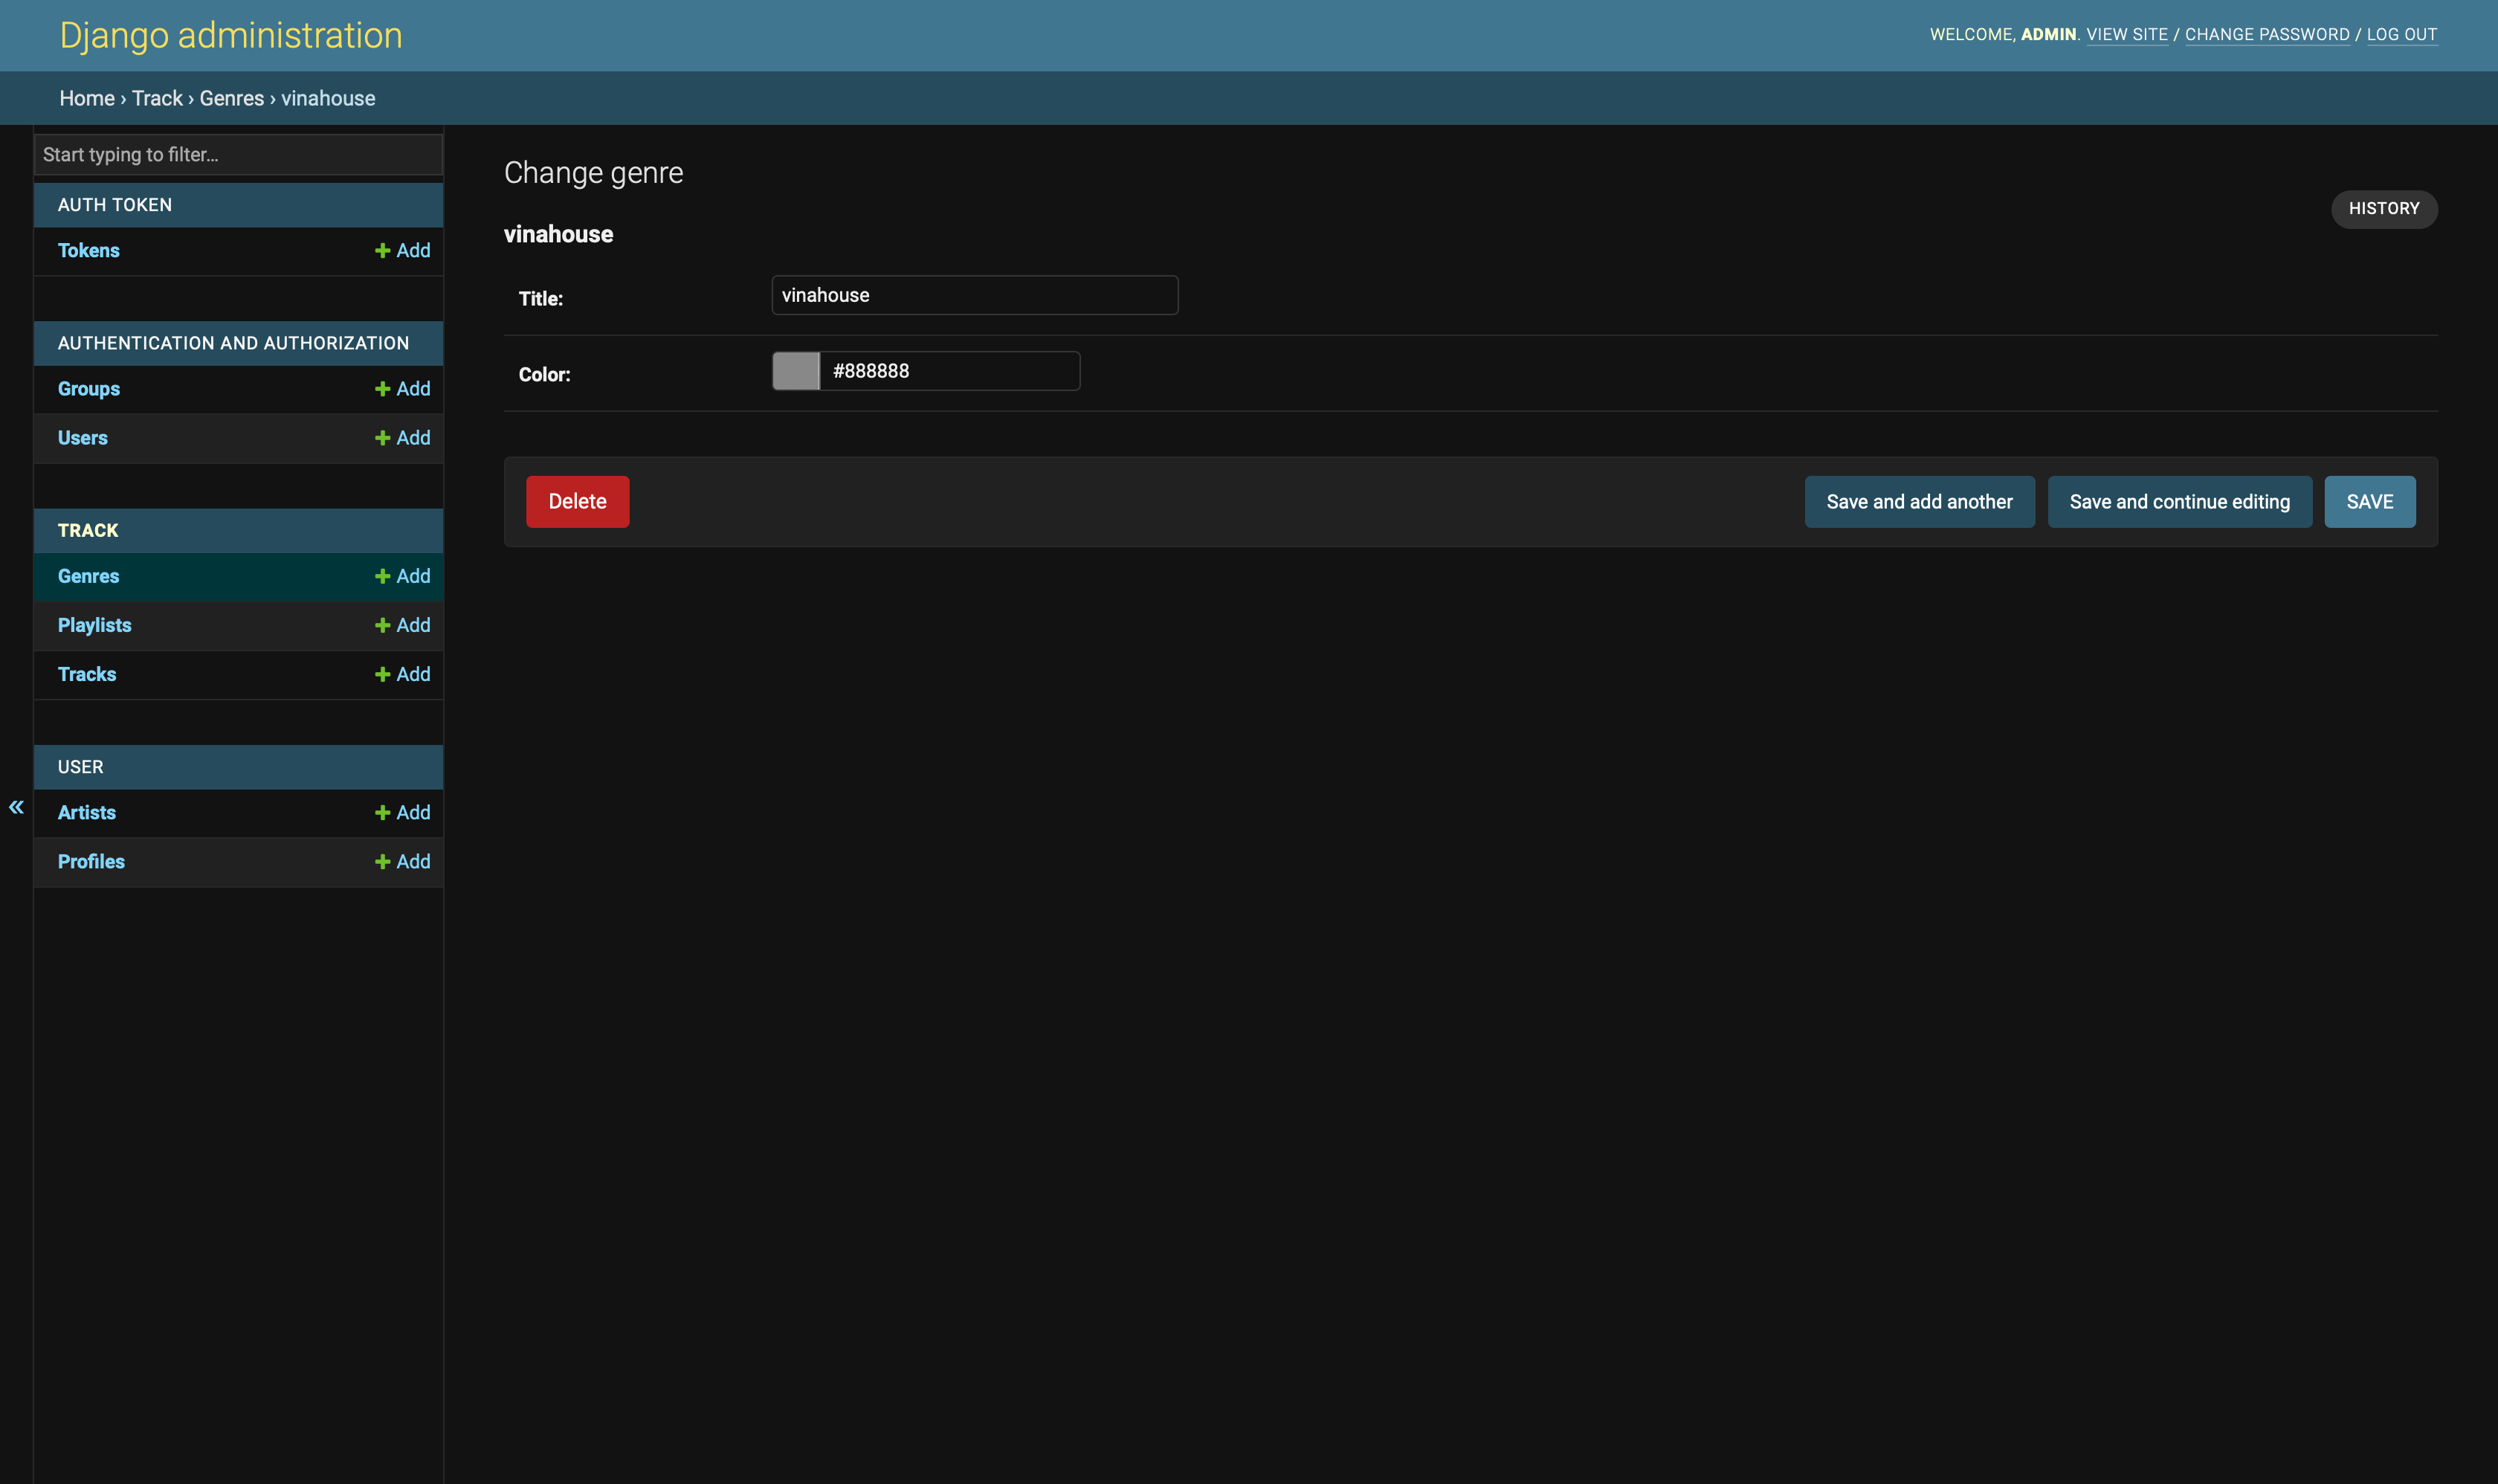
\includegraphics[width=12cm]{admin_genres_detail.png}
\end{center}
\end{figure}
\newpage

\subsubsection{Trang admin - Danh sách phát}
\begin{figure}[h!]
\begin{center}
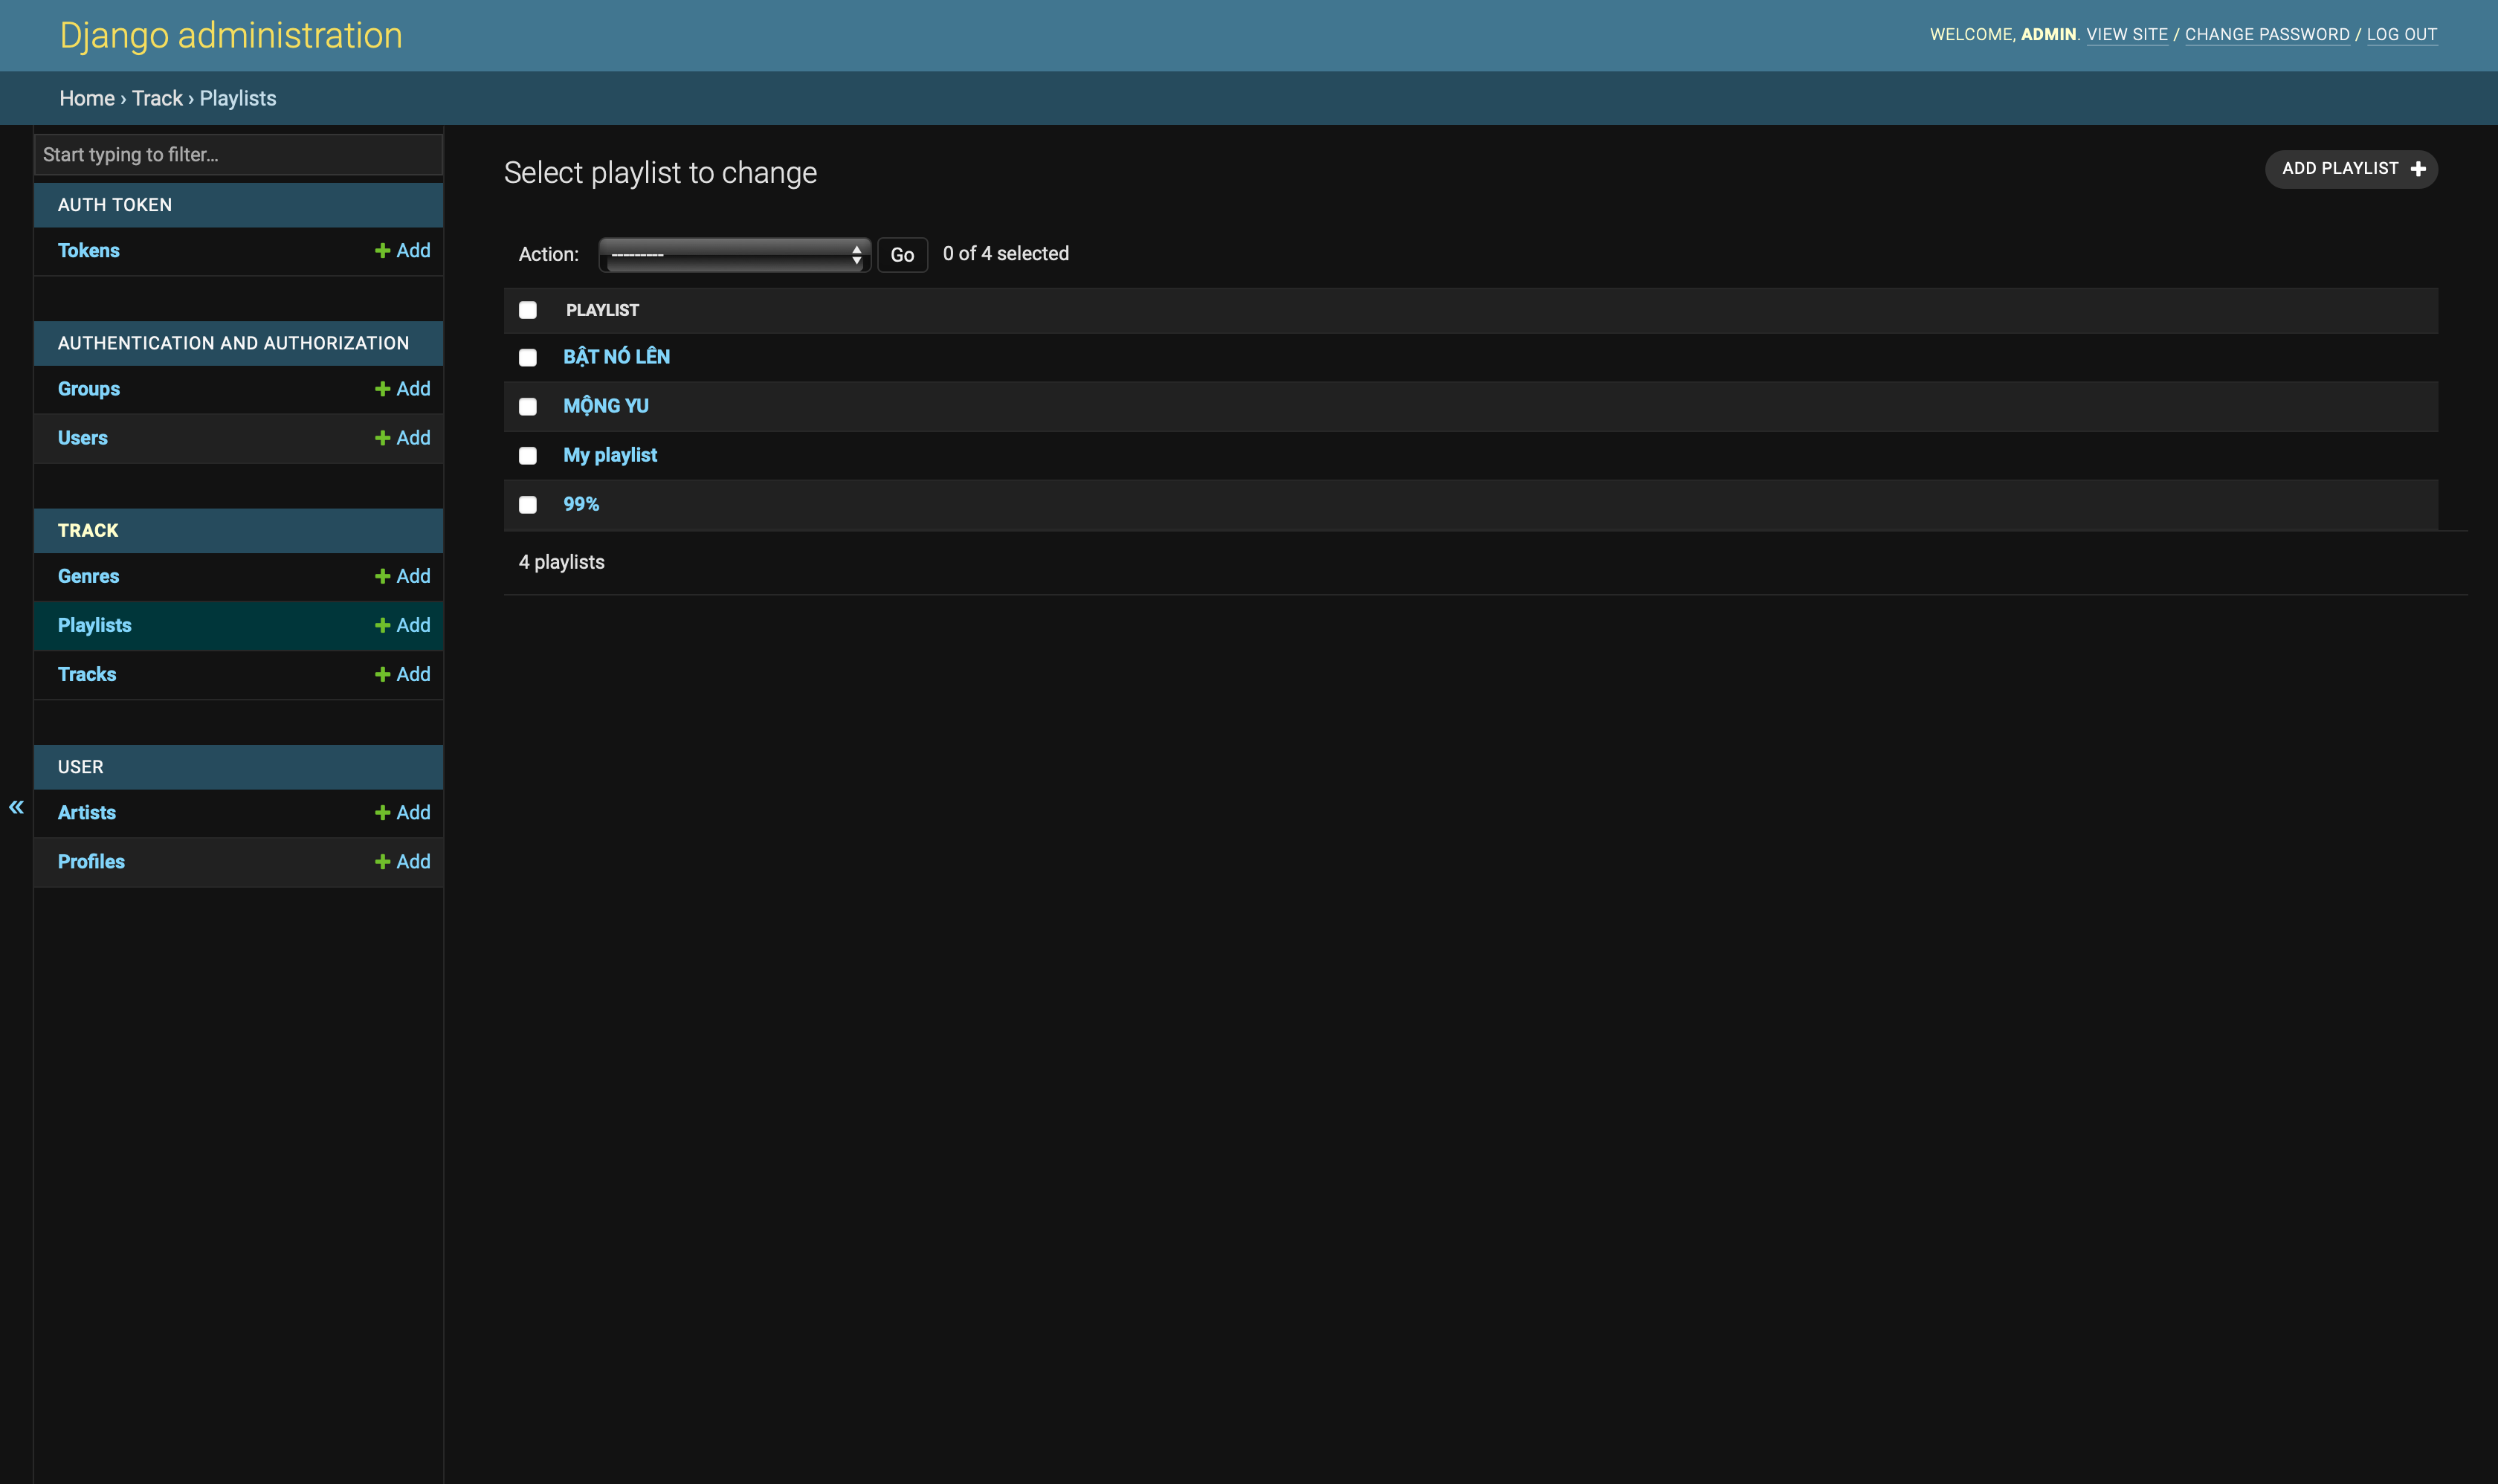
\includegraphics[width=12cm]{admin_playlist.png}
\end{center}
\end{figure}

\subsubsection{Trang admin - Chi tiết danh sách phát}
\begin{figure}[h!]
\begin{center}
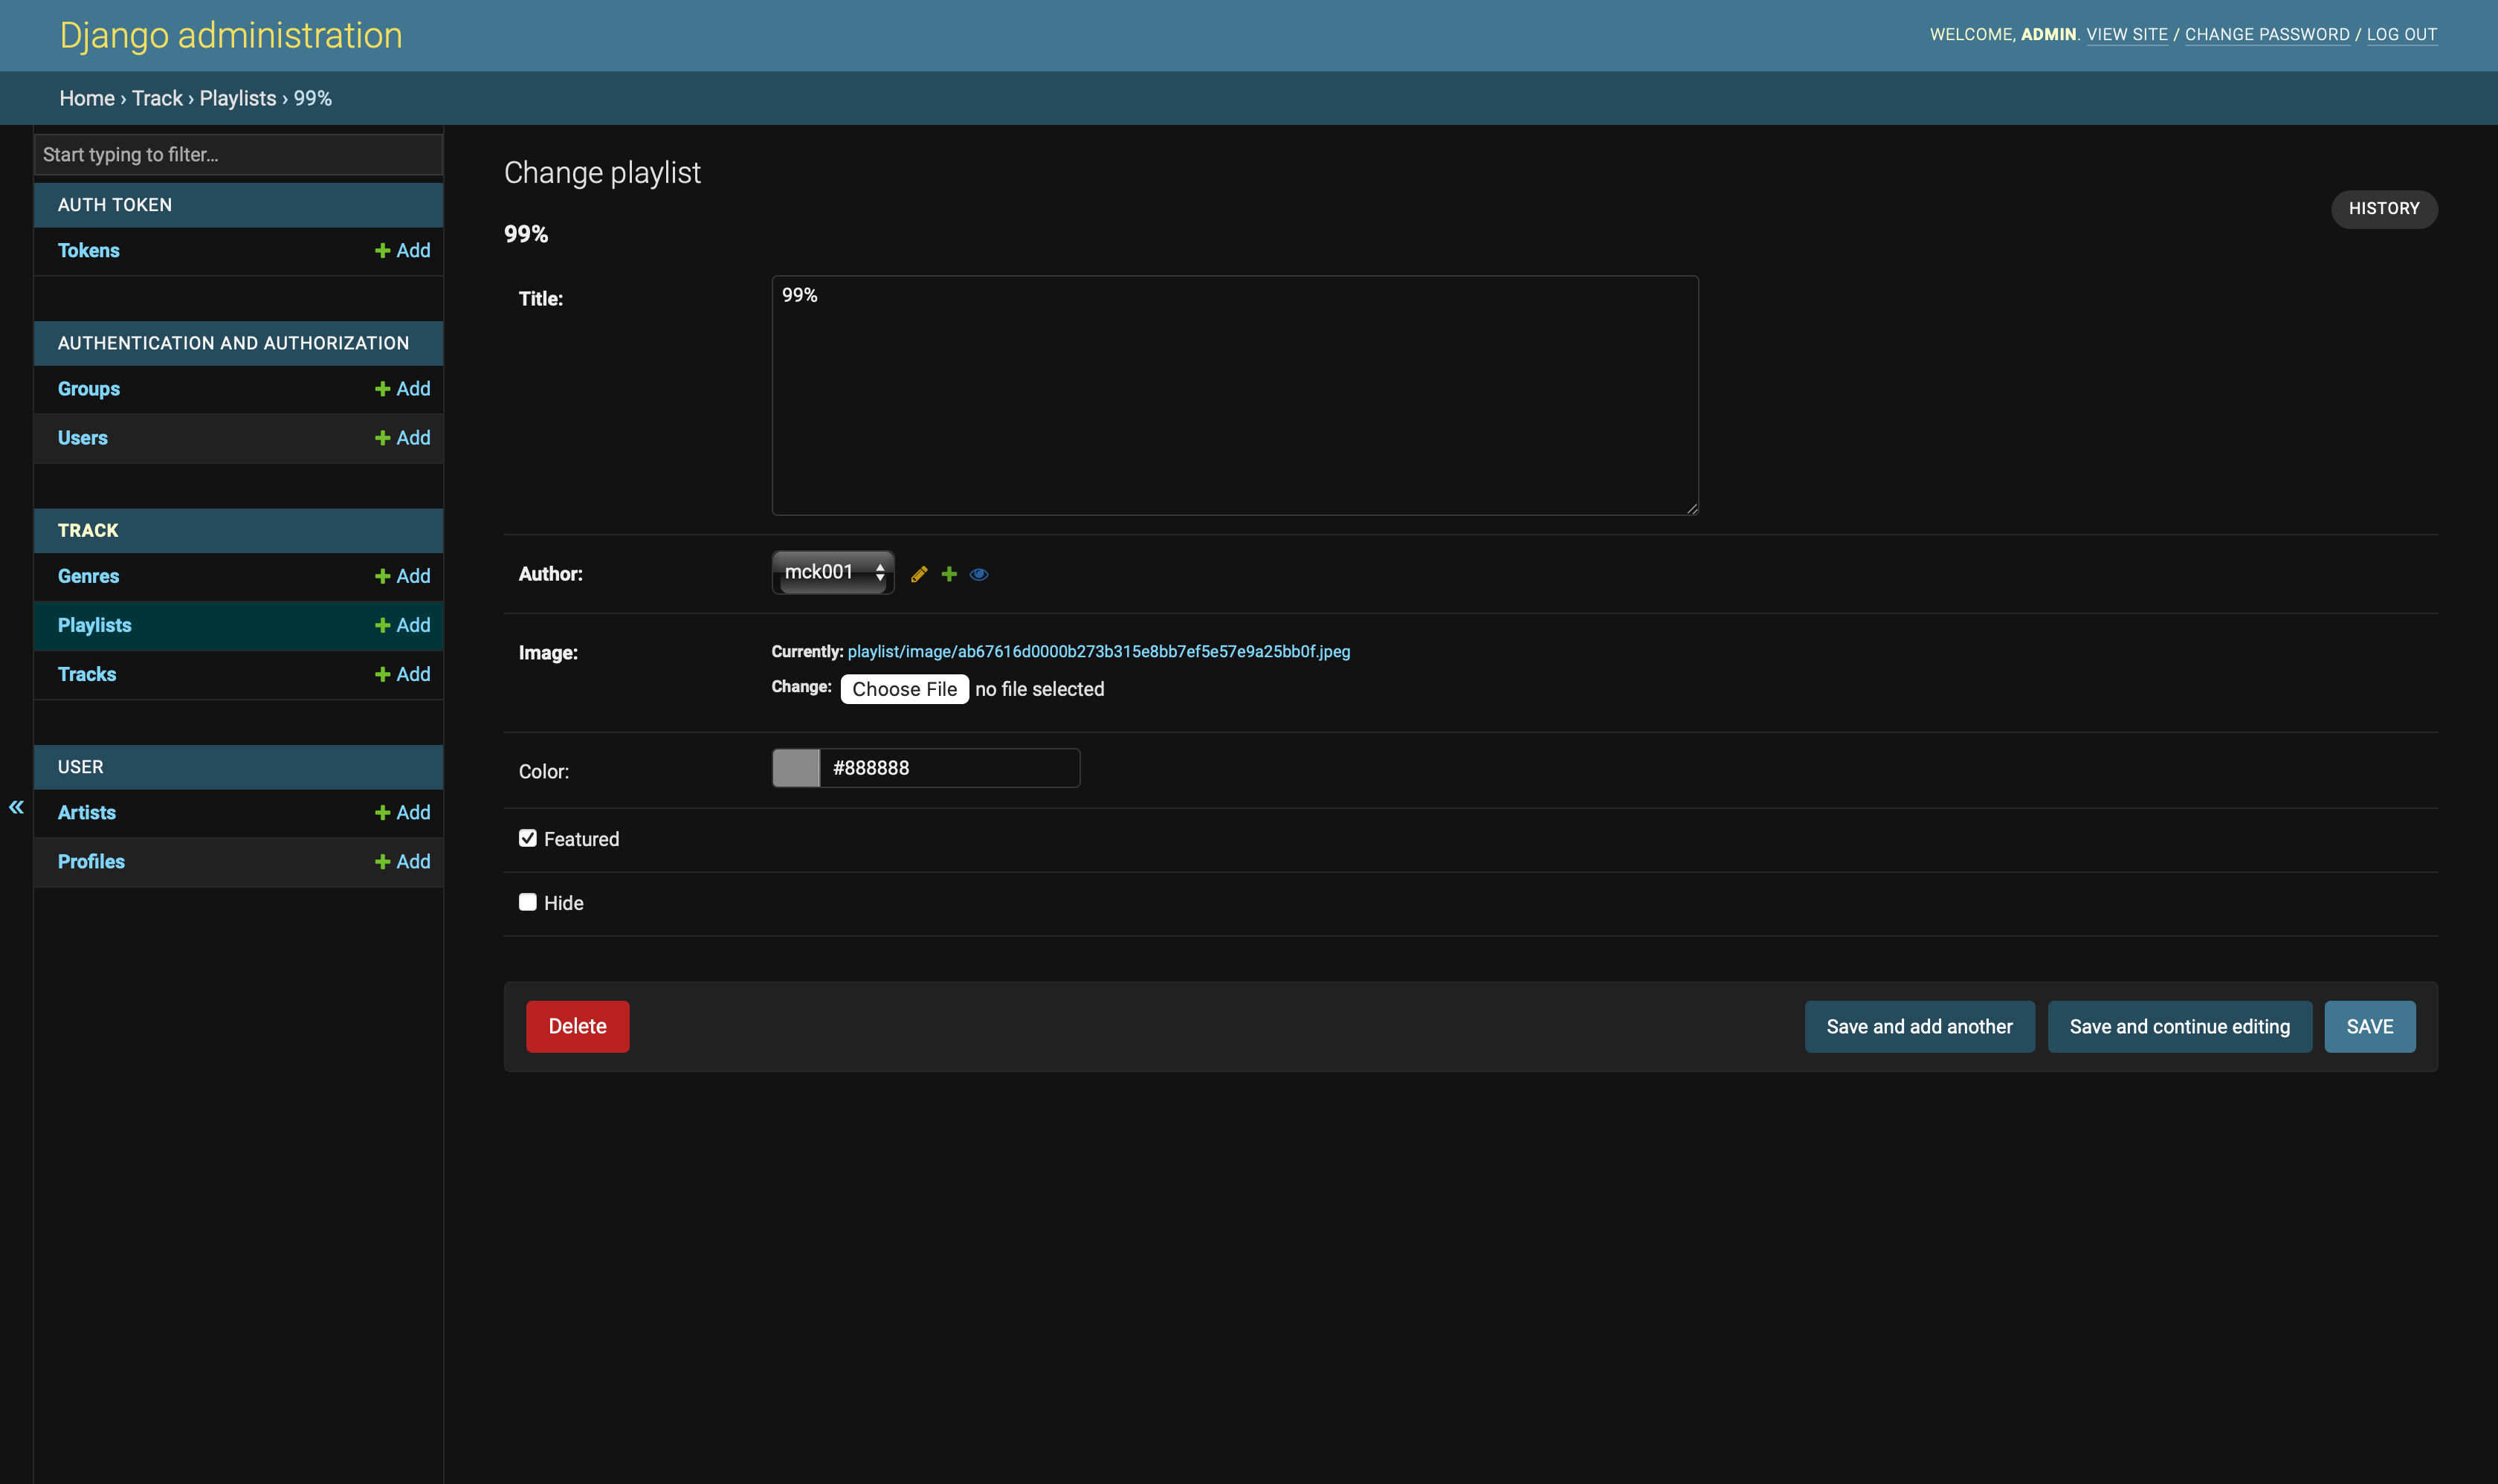
\includegraphics[width=12cm]{admin_playlist_detail.png}
\end{center}
\end{figure}
\newpage

\subsubsection{Trang admin - Bản nhạc}
\begin{figure}[h!]
\begin{center}
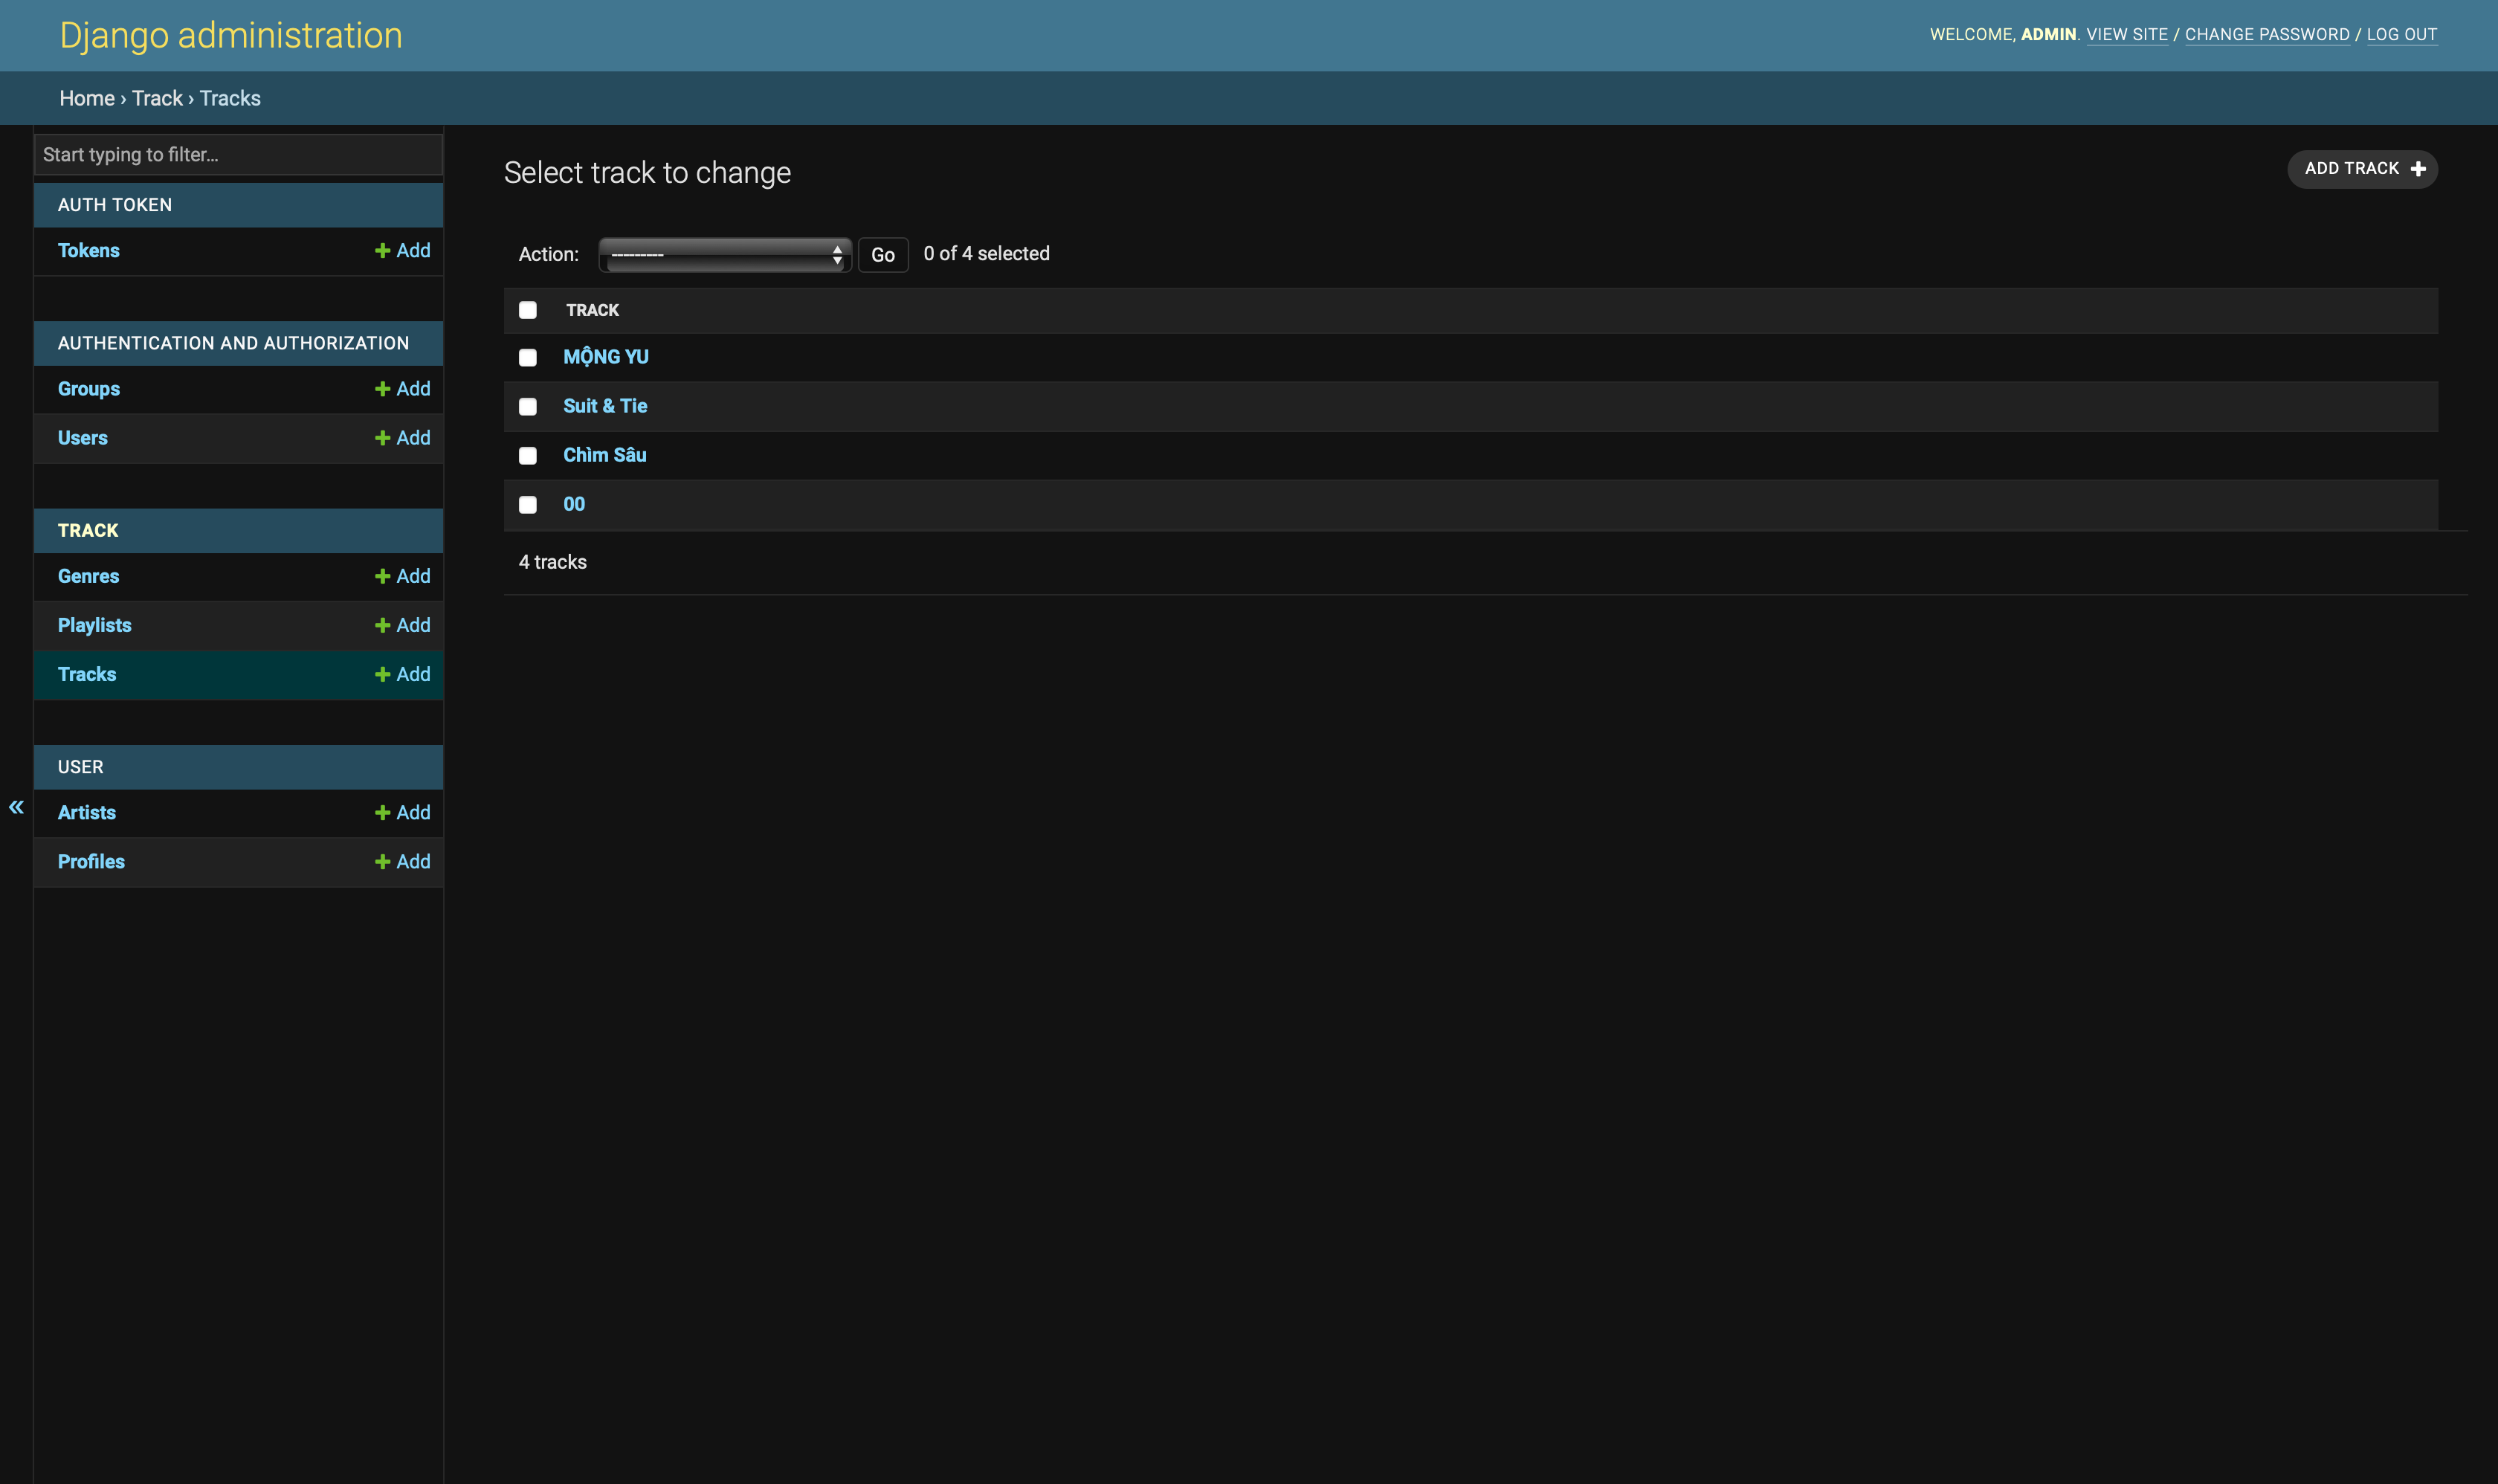
\includegraphics[width=12cm]{admin_track.png}
\end{center}
\end{figure}

\subsubsection{Trang admin - Chi tiết bản nhạc}
\begin{figure}[h!]
\begin{center}
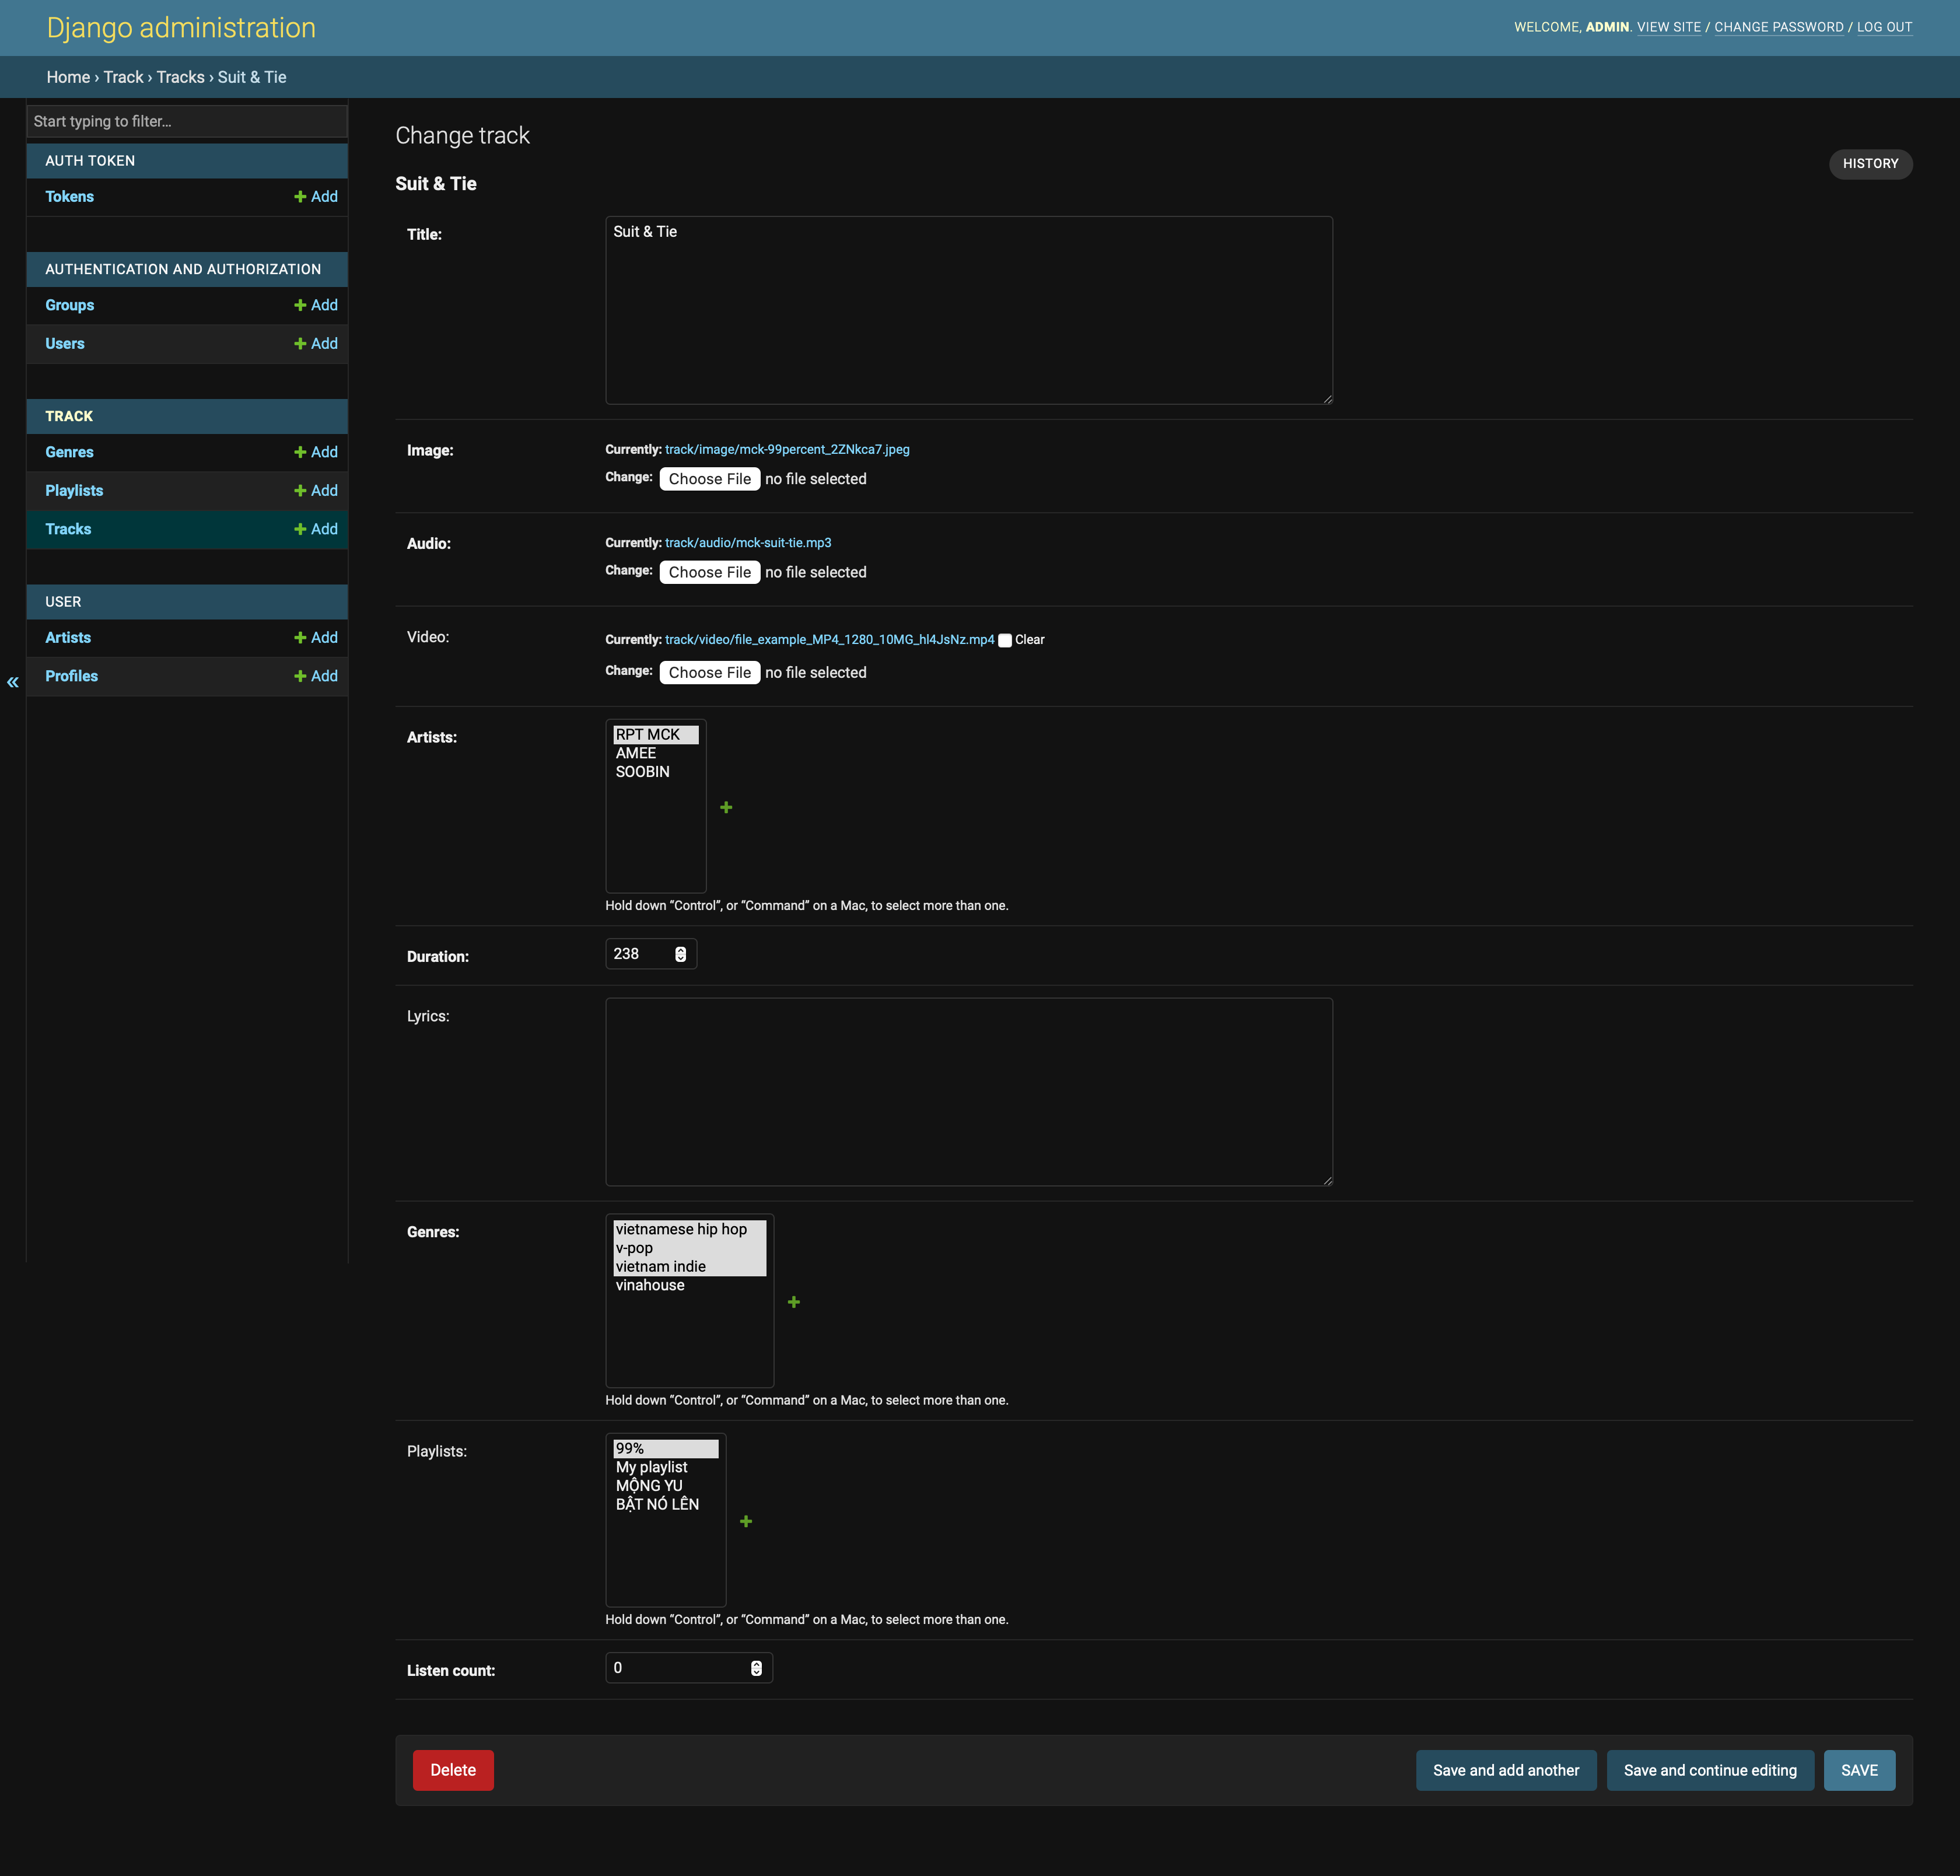
\includegraphics[width=12cm]{admin_track_detail.png}
\end{center}
\end{figure}
\newpage

\section{Hướng dẫn cài đặt}
\begin{enumerate}
    \item Cài đặt Docker
    \item Mở Terminal tại thư mục gốc mã nguồn và chạy lệnh
    \begin{lstlisting}
    docker compose -f assets/docker-compose.yml up -d
    \end{lstlisting}
    \item Truy cập trang web phần mềm tại địa chỉ http://localhost:49084/
    \item Truy cập trang web quản trị (admin) tại địa chỉ http://localhost:49088/admin/ với username và password đều là admin
\end{enumerate}

\section{Phân công}
\begin{table}[h]
    \centering
    \arrayrulecolor{black}
    \begin{tabular}{|c|c|c|c|}
        \hline
        \color{black} STT & \color{black} Thành viên & \color{black} Công việc & \color{black} Đánh giá \\
        \hline
        \color{black} 1 & \color{black} Huỳnh Xuân Bách & \color{black} Thế loại, Danh sách phát, Bài nhạc & \color{black} 50\% \\
        \hline
        \color{black} 2 & \color{black} Trần Quốc Sĩ & \color{black} Người dùng, Hồ sơ người dùng, Nghệ sĩ & \color{black} 50\% \\
        \hline
    \end{tabular}
%    \caption{Caption placeholder}
%    \label{tab:placeholder_label}
\end{table}
\newpage

\begin{thebibliography}{80}
\bibitem{DRF}
Django REST framework
``\textbf{https://www.django-rest-framework.org/}'',
\textit{}.

\bibitem{DD}
Docker Documentation
``\textbf{https://docs.docker.com/}'',
\textit{}.

\bibitem{RD}
React Documentation
``\textbf{https://devdocs.io/react/}'',
\textit{}.

\bibitem{RT}
Redux Toolkit
``\textbf{https://redux-toolkit.js.org/}'',
\textit{}.

\bibitem{MUI}
Material UI
``\textbf{https://mui.com/material-ui/}'',
\textit{}.

\bibitem{TS}
TypeScript
``\textbf{https://www.typescriptlang.org/docs/}'',
\textit{}.

\bibitem{TCD}
Tailwind CSS Documentation
``\textbf{https://v2.tailwindcss.com/docs/}'',
\textit{}.

\bibitem{VD}
Vite Documentation
``\textbf{https://vite.dev/guide/}'',
\textit{}.

\end{thebibliography}
\end{document}